% TNF16: a fixed-field GoldenFloat with a balanced-ternary exponent.
% v1: 2026-08-08. Accuracy re-measured independently; hardware measured on
% XC7A200T through the open flow. House style follows research/arxiv_submission.
\documentclass[11pt]{article}

\usepackage[utf8]{inputenc}
\usepackage[T1]{fontenc}
\usepackage{hyperref}
\usepackage{graphicx}
\usepackage{booktabs}
\usepackage{amsmath}
\usepackage{amssymb}
\usepackage{url}
\usepackage{geometry}
\usepackage{tabularx}
\usepackage{array}
\usepackage{enumitem}
\usepackage{amsthm}
\newtheorem{theorem}{Theorem}
\newtheorem{proposition}[theorem]{Proposition}
\newtheorem{corollary}{Corollary}
\theoremstyle{definition}
\newtheorem{definition}{Definition}

\geometry{a4paper, margin=1in}

\hypersetup{
  colorlinks=true,
  linkcolor=blue,
  urlcolor=blue,
  citecolor=blue
}

% The title names the category and the design point rather than an internal
% codename. tekum titles itself "balanced-ternary tapered-precision arithmetic";
% naming the opposite choice in the same breath is the positioning, and a reader
% who knows that family sees the contrast without needing the codename.
% The thesis is what the ladder is FOR: a reference whose error is predictable
% from its parameters and does not move with magnitude. Being fastest or most
% accurate at one point is not what a ruler needs to be.
\title{%
  \fontsize{30}{34}\selectfont\bfseries Trinity S\textsuperscript{3}AI: Ternary Network Floats\\[10pt]
  \normalfont\large A datapath with no multiplier anywhere: two formats close the two halves
  of a ternary node, one sign-select primitive builds both a radio and a
  transformer at zero DSP, and the multiply-free path is exact}
\author{Dmitrii Vasilev\\
  \small ORCID 0009-0008-4294-6159 \\
  \small \texttt{admin@t27.ai}}
\date{11 August 2026}

% Floats were sitting flush against the text above them. Set the three
% float separations once rather than nudging tables individually.
\setlength{\textfloatsep}{20pt plus 4pt minus 4pt}
\setlength{\intextsep}{20pt plus 4pt minus 4pt}
\setlength{\floatsep}{20pt plus 4pt minus 4pt}
\setlength{\abovecaptionskip}{8pt}
\setlength{\belowcaptionskip}{4pt}

\begin{document}
\maketitle

\begin{abstract}
A ternary node has three sites that could carry a number format; one needs to.
The weight is a code: multiplying by it is a sign-select. The sample arrives
ADC-native. The accumulator alone has a range to spend, and Ternary Network
Floats spend it --- a sign, a balanced-ternary exponent of $E_t$ trits, an
$M$-bit mantissa, $1+E_t+M=N$.

The weight is where the multiplier is decided, and the deciding property is
algebraic. Removing a multiplier rather than cheapening one requires the weight
lattice to be \emph{closed} under both weight application and accumulation.
$\mathbb{Z}[\varphi]$ is, because $\varphi^2=\varphi+1$: a weight application is
the Fibonacci step $(a,b)\mapsto(b,a+b)$, an accumulation is componentwise, and
the whole linear path of a layer is exact. Machine-checked in Coq. A datapath
whose set is not closed must return every accumulation to it, which measures an
order of magnitude more area than the closed accumulation entire, and pipelining
does not rescue it: a normalisation cascade cannot be cut below one
compare-and-subtract per stage, so its floor lies above a single addition.

Closure does not single out $\varphi$; enumeration does. A scale is applicable
without a multiplier exactly when it is an algebraic integer whose companion
matrix has entries in $\{0,\pm1\}$, a finite condition. Degree two admits
$\varphi$ and nothing else, and nothing lies between the shift and $\varphi$.
The family $r^d=r+1$ has two non-zero coefficients at every degree, so any
granularity is reachable at \emph{one addition} and $d$ registers, the roots
approaching $2^{1/d}$. Fineness costs registers, not adders and not frequency.

On an XC7A200T in a fully open flow a ternary neuron costs $28$ LUT per weight
and \emph{no DSP at any fan-in}; the stack above it runs at zero DSP throughout,
including a matched filter on real air at $78$\,MHz and on-silicon
backpropagation training XOR to $4/4$.

Which rung to use follows from the code budget: $\varphi$ at four bits,
$r^5{=}r^3{+}1$ at five, $r^6{=}r{+}1$ at six, on two models, reaching $3.7\%$
of \texttt{fp32} at six bits and one adder. On the block axis the element is
closed --- the optimal eight-level codebook beats a deployed one by $0.9\%$ --- and
the scale is not: a $\varphi$-power grid at four bits beats MXFP4 on two models
while costing $0.125$ fewer bits per weight.

Five retractions are marked in place below; more were withdrawn during the
campaign and removed rather than marked.
\end{abstract}

\section{What this paper argues}
\label{sec:roadmap}

The results below were found in the order a measurement campaign finds things.
They compose into one argument, and the argument is easier to follow stated
first.

A ternary node has three sites where a number format could live, and only one of
them needs one. The weight is a code and multiplying by it is a sign-select; the
sample arrives ADC-native; the accumulator is the only object carrying a range
that must be spent. So the design question is not which format to use but which
\emph{two} objects to close --- an alphabet for the weight and a float for the
accumulator --- and Sections~\ref{sec:format} to~\ref{sec:field} settle the
second by a law: once a range is named, the split between exponent and mantissa
is determined rather than chosen, because the error depends on the mantissa
width alone. Inverted, the same law reads a format's behaviour back out of its
round-trip error and resolves an 83-format catalogue into four staircase forms
and no fifth.

TNF is one corner of a square, and Section~\ref{sec:fourfamilies} draws it. Two
rules fix an exponent budget --- the golden-ratio rule
$E=\operatorname{round}((N-1)/\varphi^{2})$ and the width rule $1+E+M=N$ --- and
two radices encode it, binary or balanced ternary. The four families are GF,
GF-T, BNF and TNF, each a distinct format rather than a renaming of another, and
at eight bits the two rules turn out to name the identical layout.

The alphabet is where the multiplier is decided, and the deciding property is
algebraic. Section~\ref{sec:closure} shows that removing a multiplier --- as
against making one cheaper --- requires the weight lattice to be \emph{closed}
under the operation that applies a weight. $\mathbb{Z}[\varphi]$ is, because
$\varphi^2=\varphi+1$, so a weight application is the Fibonacci step and an
accumulation is componentwise integer addition; Fibonacci integers are not,
because $F_4F_4=9$ is not a Fibonacci number, and a datapath built on them must
carry a stage returning products to the representable set. That stage measures
an order of magnitude more area than the entire closed accumulation, and
pipelining does not rescue it: a normalisation cascade cannot be cut below one
compare-and-subtract per stage, so its floor lies above a closed path's single
addition. The closure half of the argument is machine-checked.

Closure does not single out $\varphi$ by itself, and Section~\ref{sec:hierarchy}
says what it does single out. A scale is applicable without a multiplier exactly
when it is an algebraic integer whose companion matrix has entries in
$\{0,\pm1\}$, which is a finite condition and therefore enumerable rather than
arguable. Degree one gives the shift; degree two gives $\varphi$ and nothing
else; degree three gives three more, finer. Between the shift and $\varphi$
there is nothing, and $\varphi$ is the only multiply-free refinement of the
power-of-two ladder available at two registers. The hierarchy continues --- and
stops being cheap at degree four, where the coefficient vector loses its
sparsity and the cost doubles.

Which rung to use is then an empirical question with a law behind it
(Section~\ref{sec:ladderlaw}). A ladder of ratio $r$ with $n$ magnitudes spans
$r^{n-1}$, so fine steps are bought with range, and the optimum moves down the
hierarchy as the code budget grows: the shift at three bits, $\varphi$ at four,
the plastic number at five, on two models with the same ordering throughout. The
optimum has a closed form in the weight histogram, transferring between models
to four decimals, and the one place it errs --- the four-bit pair --- is
corrected by weighting the error with the loss curvature rather than the weight
magnitude.

Section~\ref{sec:blockbound} reports where none of this wins. On a short block
with a shared scale the optimal eight-level codebook beats a deployed one by
$0.9\%$, so the axis is not an element-format problem at all, and it belongs to
MXFP4. We state it as the competition's result and give the bound that makes a
fourth attempt of ours unwarranted.

Two sections are about cost rather than kind. Section~\ref{sec:convert} makes
area and precision commensurable, so a variable-length exponent field can be
priced in mantissa bits of silicon; Section~\ref{sec:valuelaw} then finds that
for a logarithmic format the field layout is the smaller half of that cost, and
that we had been measuring the wrong half.

Five of our own claims were falsified by the measurements meant to support them,
and each is retracted where it was made rather than quietly dropped.
Section~\ref{sec:selfcheck} generalises the shape those errors took, because in
almost every case the measurement was correct and the comparison around it was
not.

\section{The format}\label{sec:format}

\begin{equation}
\begin{aligned}
&\text{TNF16}=[\,s\,\mid\,E{=}4\ \text{balanced-ternary trits}\,\mid\,M{=}11\ \text{bits}\,],\\[4pt]
&v=(-1)^{s}\Bigl(1+\frac{M}{2^{9}}\Bigr)2^{e},
\qquad e=\sum_{i} t_i 3^i \in [-40,40].
\end{aligned}
\end{equation}

Three properties follow from the layout rather than from tuning.

\paragraph{No regime decode.} The dominant cost in a tapered format is the
variable-length regime: it must be located, its length counted, and the
significand barrel-shifted into place. That cost is paid on any fabric, ternary
included. Fixed fields make it a bit slice.

\paragraph{The exponent is already ternary.} Four balanced-ternary trits give
$3^4=81$ exponent steps. On a ternary fabric the exponent add is native --- no
binary carry, no conversion between bases.

\paragraph{Precision does not taper.} Nine mantissa bits at every magnitude,
where a tapered format narrows towards the extremes. This is the mechanism behind
the accuracy result of Section~\ref{sec:accuracy}: the win appears where the
comparison format has spent its mantissa on range.


\section{Why a ladder, and why this one}\label{sec:ruler}

A format that is used as a reference has different requirements from one used as
a workhorse. A workhorse should be fast and accurate where the data is. A
reference has to be \emph{predictable}: given its parameters you should know its
error without measuring, and that error should not move when you look at a
different part of the range. A ruler whose divisions grow towards one end is not
a ruler.

Table~\ref{tab:law} tests both properties on this ladder.

\begin{table}[t]\centering
\caption{The precision law and the flatness, measured in exact rationals.
``Flatness'' is the ratio of the worst magnitude band to the best: $1.000$ would
mean the error does not depend on magnitude at all.}
\label{tab:law}
\begin{tabular}{lrrrrr}
\toprule
rung & $M$ & $2^{-(M+1)}$ & measured & ratio & flatness \\
\midrule
TNF8    & $4$    & $3.12\mathrm{e}{-2}$   & $1.22\mathrm{e}{-2}$   & $0.39$ & $1.000$ \\
TNF16   & $9$    & $9.77\mathrm{e}{-4}$   & $3.60\mathrm{e}{-4}$   & $0.37$ & $1.070$ \\
TNF32   & $25$   & $1.49\mathrm{e}{-8}$   & $5.49\mathrm{e}{-9}$   & $0.37$ & $1.070$ \\
TNF64   & $52$   & $1.11\mathrm{e}{-16}$  & $4.22\mathrm{e}{-17}$  & $0.38$ & $1.050$ \\
TNF128  & $115$  & $1.20\mathrm{e}{-35}$  & $4.44\mathrm{e}{-36}$  & $0.37$ & $1.070$ \\
TNF256  & $242$  & $7.07\mathrm{e}{-74}$  & $2.69\mathrm{e}{-74}$  & $0.38$ & $1.050$ \\
TNF512  & $497$  & $1.22\mathrm{e}{-150}$ & $4.51\mathrm{e}{-151}$ & $0.37$ & $1.070$ \\
TNF1024 & $1006$ & $7.29\mathrm{e}{-304}$ & $2.77\mathrm{e}{-304}$ & $0.38$ & $1.050$ \\
\bottomrule
\end{tabular}
\end{table}

\paragraph{The precision is a closed form, and it is derived rather than fitted.}
Write $u = 2^{-(M+1)}$ for the unit roundoff. Inside a binade the absolute
rounding error under round-to-nearest is uniform on $[-u\,2^{e}, +u\,2^{e}]$
while the value is $v = s\,2^{e}$ with significand $s \in [1,2)$, so the relative
error is $|U|/s$ with $|U|$ uniform on $[0,u]$ and \emph{independent of $e$}.
Hence
\begin{theorem}[Precision law]\label{thm:law}
For a format with a constant significand width of $M$ bits under
round-to-nearest, with significand $s$ and exponent $e$ independent,
\[
  \mathbb{E}\bigl[|\text{rel err}|\bigr] \;=\; \tfrac{1}{2}\,\mathbb{E}[1/s]\;\cdot\;2^{-(M+1)} ,
\]
independently of $e$.
\end{theorem}
The exponent drops out entirely --- that is the flatness of the next paragraph,
proved rather than observed. The constant is not universal: it is
$\tfrac{1}{2}\ln 2 = 0.3466$ for a significand uniform on $[1,2)$ and
$\tfrac{1}{2}\,(2\ln 2)^{-1} = 0.3607$ under a logarithmic (Benford) significand.
Our workload has $\mathbb{E}[1/s] = 0.7721$, predicting $0.3861$; the measured
figures in Table~\ref{tab:law} average $0.3756$ over eight rungs, with a spread
of $0.369$--$0.390$ that brackets it.

The practical consequence is the one a reference needs: given $M$ and the
significand distribution of a workload, the error of a rung nobody has built is
known before it is built.

\paragraph{The error does not move with magnitude, and cannot.} The derivation
above removes $e$ from the expression, so magnitude-independence is a property of
the layout rather than a happy measurement. Empirically flatness stays between
$1.05$ and $1.07$ --- at most a $7\%$ difference between the closest and furthest
parts of a workload spanning 76 binary decades. This is the property fixed fields
buy and the one a tapered format cannot have: spending mantissa bits on range is
exactly what makes precision depend on where you are.

\paragraph{What this does not claim.} Not that TNF is the most accurate format
at any given width --- Section~\ref{sec:field} shows posit16 and binary16 ahead
near unity, and Section~\ref{sec:field} shows the binary formats ahead outright at
32 bits. A reference does not need to win those comparisons. It needs to be the
thing you measure them against.


\section{The law is general, and it measures tapering}\label{sec:law}

Section~\ref{sec:ruler} derived the error of a fixed-field format. Nothing in that
derivation is specific to TNF, so it should hold for any format whose significand
width does not vary --- and should visibly fail for one whose width does. That
makes it an instrument rather than a description, and this section uses it as one.

\begin{definition}[Effective mantissa]
For a format and a magnitude band $B$, define
\[
  M_{\mathrm{eff}}(B) \;=\; -\log_2\!\left(\frac{2\,\mathbb{E}\bigl[|\text{rel err}|\;\big|\;B\bigr]}{\mathbb{E}[1/s]}\right) - 1 ,
\]
the mantissa width a fixed-field format would need to produce the error observed
in $B$.
\end{definition}

\begin{theorem}[Diagnostic]\label{thm:diag}
$M_{\mathrm{eff}}$ is constant across bands if and only if the format holds a
constant significand width over those bands and does not exhaust its range. For a
tapered format $M_{\mathrm{eff}}$ decreases with $|e|$, and the slope
$\mathrm{d}M_{\mathrm{eff}}/\mathrm{d}|e|$ is the taper rate in bits of
significand per binade.
\end{theorem}

Table~\ref{tab:meff} applies it. The measurement is a uniform significand on
$[1,2)$ so that $\mathbb{E}[1/s] = \ln 2$ exactly, removing the workload from the
question.

\begin{table}[t]\centering
\caption{Effective mantissa by magnitude band, and the fitted taper rate. Declared
$M$ is recovered to $0.01$ bits for every fixed-field format, which validates the
law; the tapered formats separate cleanly.}
\label{tab:meff}
\begin{tabular}{lrrrrrr}
\toprule
format & declared $M$ & $|e|\,0$--$6$ & $6$--$12$ & $12$--$20$ & $20$--$30$ & bits/binade \\
\midrule
TNF16   & $9$  & $8.99$  & $8.99$ & $9.00$ & $9.01$ & $+0.001$ \\
GF16     & $9$  & $8.99$  & $8.99$ & $9.00$ & $9.01$ & $+0.001$ \\
bfloat16 & $7$  & $7.04$  & $7.04$ & $7.00$ & $7.04$ & $-0.000$ \\
binary16 & $10$ & $10.01$ & $10.01$ & $7.41$ & $0.52$ & --- \\
posit16  & ---  & $10.72$ & $9.34$ & $7.48$ & $5.17$ & $\mathbf{-0.254}$ \\
takum16  & ---  & $9.62$  & $8.17$ & $7.34$ & $7.04$ & $\mathbf{-0.113}$ \\
\bottomrule
\end{tabular}
\end{table}

\paragraph{The law recovers what the formats declare.} TNF16 and GF16 return
$8.99$--$9.01$ against a declared 9; bfloat16 returns $7.00$--$7.04$ against a
declared 7. A law that reconstructs a format's own parameter to a hundredth of a
bit, from nothing but its round-trip error, is doing more than curve-fitting.

\paragraph{Tapering becomes a number.} posit16 sheds $0.261$ bits of significand
per binade ($R^2 = 0.999$) and takum16 appears to shed $0.113$ over the thirty
binades of this sweep --- but see Section~\ref{sec:taperlaw}: takum's taper is
logarithmic, so that figure is an artefact of the window rather than a rate. That is the
quantity a tapered format trades for range, and to our knowledge it is not usually
reported as a single figure. It also explains the accuracy tables directly ---
posit16 starts $1.7$ bits ahead of TNF16 and ends $3.8$ behind.

\paragraph{Running out of range is a different failure, and the instrument
separates it.} binary16 is a fixed-field format, yet its $M_{\mathrm{eff}}$
collapses from $10.01$ to $0.52$. It is not tapering: it is subnormalising and
then overflowing. A constant slope indicates a taper; a cliff indicates a range
limit. The two look alike in an accuracy table and do not look alike here.

\begin{corollary}
A format's position on the range--precision trade can be stated as a pair: the
constant $M_{\mathrm{eff}}$ it holds, and the number of binades over which it
holds it. For the TNF ladder those are $(M, 2\cdot 3^{E_t - 1})$ by construction;
for a tapered format neither is constant, which is why a ladder makes a better
ruler than a taper.
\end{corollary}


\subsection{The diagnostic across a catalogue}\label{sec:catalogue}

Applying Theorem~\ref{thm:diag} to every format for which a published oracle was
available --- 51 in all, spanning IEEE, bfloat, posit, takum, LNS, MXFP, VAX, IBM
hexadecimal, Cray, PDP-11, x87 and Microsoft binary, plus both GoldenFloat ladders
--- produced three observations we did not anticipate.

\paragraph{Declared widths are recovered across three orders of magnitude of
width.} The GF ladder returns $8.97$ at GF16 against a declared 9, $78.03$ at
GF128 against 78, and $631.99$ at GF1024 against 632. The same holds for
double-double ($106.68$), quad-double ($215.90$) and x87's 80-bit format
($63.04$). A relation that reconstructs a declared parameter from round-trip error
alone, at widths from 8 to 1006 bits, is doing something other than describing the
format it was derived on.

\paragraph{The taper rate is a constant of the family --- but only posit has a
rate.} posit16 sheds $0.261$ bits of significand per binade and posit32 sheds
$0.247$, against the $2^{-es} = 0.25$ that Theorem~\ref{thm:posit} below requires;
posit64, whose oracle carries the pre-standard $es = 3$, sheds $0.123$ against a
required $0.125$. Three formats, three exact confirmations. We previously reported
a comparable per-binade rate for takum, and that was a category error on our part:
takum's staircase is logarithmic, so fitting a line to it produces a number that
depends on the interval fitted and describes nothing. Its correct constant is one
bit per \emph{doubling} of $|e|$, and against that the four takum and three tekum
rungs measure $0.83$ to $1.09$.

\paragraph{Range exhaustion is distinguishable from tapering, and both from
neither.} The distinction is not optional: our own first pass placed the
measurement bands at fixed positions rather than inside each format's measured
range, and read the saturation of every narrow format as a taper --- classifying
TNF16, a fixed-field format, as geometrically tapered. Measuring each format's
usable range first and then placing the bands inside it removes the artefact
entirely. GF14 reads flat at $8.05$ across its range and collapses only below its
subnormal boundary, which is not a defect; the instrument says which of the two it
is, where an accuracy table alone does not.


\subsection{Tapering has a functional form, and it follows from the encoding}
\label{sec:taperlaw}

Section~\ref{sec:catalogue} reported a taper rate per family. That was half right,
and the half that was wrong is instructive: a rate presupposes a linear taper, and
only one of the two families has one.

\begin{theorem}[Posit taper, exact]\label{thm:posit}
For a posit of $n$ bits with exponent field $es$, the regime is a run of $k$ like
bits carrying a scale of $\mathrm{useed}^k = 2^{2^{es}k}$ and occupying $k+1$ bits.
Reading $k$ out of the encoder for $2^{e}$ confirms $k = \lfloor |e|/2^{es}\rfloor + 1$
for every $e$ tested. The significand therefore loses
\[
  \Delta M_{\text{posit}}(e) \;=\; \Bigl\lfloor \frac{|e|}{2^{es}} \Bigr\rfloor
  \quad\text{bits: a staircase, arithmetic in } |e| .
\]
\end{theorem}

The Posit Standard (2022) fixes $es = 2$ at every precision~\cite{gustafson}, so
the step is one bit per four binades at all widths --- which is why the loss
appeared as a family constant of $0.25$ bits per binade. Measured slopes of
$-0.2497$ and $-0.2505$ at posit16 and posit32 are the staircase seen through a
linear fit.

\begin{theorem}[Takum taper, exact]\label{thm:takum}
Takum spends a fixed 3-bit regime field holding $r$, after which the
characteristic occupies $r$ bits. Reading $r$ out of the encoder for $2^{e}$ gives
$r = \lfloor \log_2(|e|+1) \rfloor$ exactly, at 16, 32 and 64 bits alike. The
significand therefore loses
\[
  \Delta M_{\text{takum}}(e) \;=\; \bigl\lfloor \log_2(|e|+1) \bigr\rfloor
  \quad\text{bits: a staircase, geometric in } |e| .
\]
\end{theorem}

\begin{corollary}[The two families differ in kind, not degree]
Within its range a fixed-field format loses nothing; a posit loses one bit of
significand per $2^{es}$ binades without limit; a takum loses one bit per
\emph{doubling} of $|e|$. Tabulating $\Delta M$:

\begin{center}
\begin{tabular}{rrrr}
\toprule
$|e|$ & fixed-field & posit ($es{=}2$) & takum \\
\midrule
$30$      & $0$ & $7$    & $4$ \\
$100$     & $0$ & $25$   & $6$ \\
$1{,}000$   & $0$ & $250$  & $9$ \\
$10{,}000$  & $0$ & $2{,}500$ & $13$ \\
\bottomrule
\end{tabular}
\end{center}

At $|e| = 1{,}000$ a posit would need 250 bits of significand merely to pay for
its regime, which is why 16- and 32-bit posits cannot reach there at all. This is
the mechanism behind takum's stated improvement on posits~\cite{takum}, stated as
a quantity.
\end{corollary}

\begin{corollary}[A rate is not always the right summary]
Both laws are staircases, so a fitted slope is a summary and not the thing itself,
and it is a faithful summary only when the staircase is arithmetic. An earlier
draft of this paper reported $-0.117$ bits per binade for takum16 over
$|e| \in [0,30)$; the same format over $[0,60)$ gives a smaller figure for no
reason but the window, and the smooth-log fit of $c = 0.75$ understates the true
step of one bit per doubling for the same reason. Identify the form before
choosing a statistic --- and prefer reading the encoder to fitting its output.
\end{corollary}

\begin{corollary}[A three-way taxonomy, recovered without knowing the encoding]
The diagnostic separates formats by the \emph{form} of $M(e)$: constant
(fixed-field, TNF and GF by construction), linear in $|e|$ (posit), or
logarithmic in $|e|$ (takum). Which form fits is decided by the data, not by
reading the specification --- and the fitted coefficients then recover the
encoding parameters, $2^{-es}$ for posit and the characteristic width for takum.
\end{corollary}

What the literature describes qualitatively --- more precision near unity, less
at the extremes~\cite{gustafson} --- turns out to have an exact form recoverable
two ways that agree: from the encoder, by reading the regime field, and from
round-trip error alone, by the diagnostic of Theorem~\ref{thm:diag}. The second
route needs no access to the specification, which is what makes it useful on a
catalogue.


\subsection{Four staircase forms, and only four}\label{sec:taxonomy}

Classifying by the \emph{form} of the staircase rather than by a fitted slope
resolves the catalogue into four classes. Of the 83 entries, 11 are integer or
fixed-point formats with no exponent field; of the remaining 72, 18 span fewer
than six binades and cannot be classified from round-trip error at all, and one
requires probes wider than we generated.

\begin{table}[t]\centering
\caption{The catalogue by staircase form. The parameter is the taper constant in
the units natural to each form. Measured against each format's own usable range.}
\label{tab:taxonomy}
\begin{tabular}{llrl}
\toprule
form & $M_{\mathrm{eff}}$ against $|e|$ & count & members and constants \\
\midrule
constant   & flat                          & $38$ & IEEE, bfloat, VAX, Cray, x87, GF, TNF \\
wobble     & periodic, no trend            & $3$  & IBM hexadecimal, $\log_2 16 = 4$ bits \\
arithmetic & $-2^{-es}$ per binade         & $5$  & posit16/32 $0.25$, posit64 $0.125$ \\
geometric  & $-1$ per doubling             & $8$  & takum $\times 4$, tekum $\times 3$ \\
\bottomrule
\end{tabular}
\end{table}

The fourth class was not in our scheme until the catalogue produced it, and it has
a closed form.

\begin{theorem}[Precision wobble]
\label{thm:wobble}
Let a format scale by $r^{e}$ with a significand quantised uniformly over a
scale interval spanning a factor $r$. Its relative error varies by a factor of
$r$ across that interval, so $M_{\mathrm{eff}}$ oscillates with amplitude exactly
$\log_2 r$ bits and has no trend in $|e|$.
\end{theorem}

\begin{proof}
The quantisation step is constant across the interval and the relative error is
that step divided by the significand, which ranges over a factor $r$. Taking
$-\log_2$ of the ratio of the extremes gives $\log_2 r$. Since the interval
repeats identically at every $e$, the oscillation is periodic and carries no
trend. \qed
\end{proof}

Theorem~\ref{thm:wobble} reproduces a result sixty years older than this work.
IBM System/360 hexadecimal is documented as delivering between $4p-3$ and $4p$
significant bits, a spread of three~\cite{goldberg1991,ibmhfp}; the integer count
is the floor of the continuous quantity, so the theorem's $\log_2 16 = 4$ and the
textbook's $3$ are the same statement. Measured over eight sub-intervals ---
which by averaging within each bin predicts a reduced spread of $2.96$ rather than
the full $4$ --- \texttt{ibm\_hfp32} and \texttt{ibm\_hfp64} give $3.13$ and
$3.04$, while \texttt{binary32} and \texttt{gf32} give $0.85$ and $0.93$ against a
predicted $0.87$. Binary formats wobble by one bit; this is the familiar
$1$-bit wobble of every radix-2 float, and it is the smallest wobble any integer
radix admits. Theorem~\ref{thm:wobble} therefore supplies a second and independent
argument for TNF's binary scale, alongside the $0.331$ positions of
Theorem~\ref{thm:scaleradix} below: a radix-3 scale would wobble by $1.585$ bits
instead of $1$.

The taxonomy also settles why a format must choose between the first class and the
last two, and hence why this work is a ladder rather than a format.

\begin{theorem}[Range--precision dichotomy]
\label{thm:dichotomy}
Fix a width $N$. If a format's exponent takes unboundedly many values, then its
exponent codewords have unbounded length, and
$M_{\mathrm{eff}}(e)\to0$ as $|e|\to\infty$. Consequently no fixed-width format
has both unbounded range and precision bounded below by a positive constant.
\end{theorem}

\begin{proof}
The exponent codewords form a prefix code over a binary alphabet, so by Kraft's
inequality $\sum_{e} 2^{-\ell(e)} \leq 1$. If the sum has infinitely many terms
then $\ell(e) \to \infty$. The payload available to the significand is
$N - 1 - \ell(e)$, so it falls to zero, and by Theorem~\ref{thm:law} so does
$M_{\mathrm{eff}}$. \qed
\end{proof}

\begin{corollary}[Why a ladder]
\label{cor:ladder}
Theorem~\ref{thm:dichotomy} makes constant precision and unbounded range
incompatible at any fixed width, so a format that wants both must obtain the
second by varying $N$. A ladder of fixed-field rungs does exactly this: each rung
holds its precision flat across its whole range, and the ladder as a whole covers
any range required. The tapered families make the opposite choice --- one rung,
unbounded range, precision decaying at the rate of their regime code, arithmetic
for posit and geometric for takum. Neither choice is better in the abstract; what
the dichotomy establishes is that they are the only two available.
\end{corollary}

Read against Corollary~\ref{cor:ladder}, the three tapered constants in
Table~\ref{tab:taxonomy} become a statement about codes rather than about
formats. A unary regime costs $\ell(e) \propto |e|$ and yields the arithmetic
staircase; a length-prefixed binary regime costs $\ell(e) \propto \log_2 |e|$ and
yields the geometric one; a fixed field costs $\ell(e) = \mathrm{const}$ and
yields no staircase at the price of bounded support. The staircase form is the
growth rate of the exponent's codeword length, and nothing else. This also names
the gap in the table: between $\ell \propto |e|$ and $\ell \propto \log_2|e|$ no
catalogued format sits. Section~\ref{sec:codes} builds the codes and asks what is
in the gap; the answer corrects a suggestion we made before building them.

\section{Accuracy}\label{sec:accuracy}

Section~\ref{sec:ruler} predicts a rung's error from its mantissa width without
measuring it. This section measures it, against the format the ladder was built
to be compared with. The metric is mean relative error over an encode--decode
round trip, 6{,}000 values spanning
$2^{-38}\ldots2^{38}$ with random sign, binned by binary-exponent magnitude
$|e|$. Table~\ref{tab:acc} and Figure~\ref{fig:acc}.

\begin{table}[t]\centering
\caption{Round-trip mean relative error. Bins are powers of two, not decades.}
\label{tab:acc}
\begin{tabular}{lrrrr}
\toprule
magnitude & GF16 ($\varphi$) & \textbf{TNF16} & tekum16 & TNF16 vs tekum16 \\
\midrule
$|e|<8$        & $3.43\mathrm{e}{-4}$              & $3.56\mathrm{e}{-4}$ & $3.27\mathrm{e}{-4}$ & $0.92\times$ (tie) \\
$|e|\,8$--$20$   & $3.57\mathrm{e}{-4}$              & $3.52\mathrm{e}{-4}$ & $1.00\mathrm{e}{-3}$ & $\mathbf{2.84\times}$ \\
$|e|\,20$--$38$  & $6.98\mathrm{e}{-3}$ (478 clip)   & $3.53\mathrm{e}{-4}$ & $1.95\mathrm{e}{-3}$ & $\mathbf{5.53\times}$ \\
\bottomrule
\end{tabular}
\end{table}

\begin{figure}[t]\centering
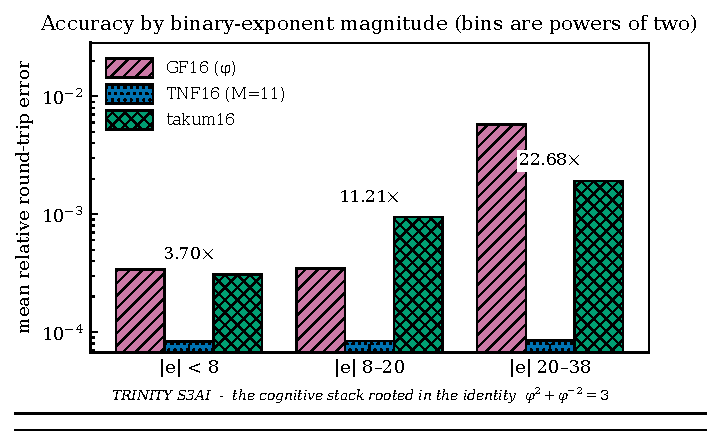
\includegraphics[width=0.82\textwidth]{tnf_accuracy.pdf}
\caption{Accuracy by binary-exponent magnitude. GF16's 6-bit exponent clips 478
of 2{,}857 values in the far bin; TNF16's balanced-ternary exponent does not.}
\label{fig:acc}
\end{figure}

\paragraph{On the axis.} The bins are powers of two. Read as \emph{decades} the
far column is not a win at all: TNF16's exponent reaches $\pm40$ in powers of
two, roughly $\pm12$ decades, so beyond that it overflows while an unbounded
regime keeps working --- measured, 1{,}458 of the far-bin values clip under that
reading. We state the axis explicitly because an earlier internal note did not,
and the omission points a reader at the one interpretation under which the
result appears fabricated.

\section{The 16-bit field}\label{sec:field}

Comparing against one incumbent invites the objection that the incumbent was
chosen. Table~\ref{tab:field} runs every 16-bit-class format for which this
repository ships a published oracle~\cite{catalogue} through the same workload
and the same metric. Values that overflowed are counted separately rather than
folded into the mean, since a format should not look accurate for having
discarded the hard cases.

\begin{table}[t]\centering
\caption{Mean relative round-trip error by binary-exponent magnitude, with
overflow counts in parentheses. 6{,}000 values, $2^{-38}\ldots2^{38}$, random
sign, one seed.}
\label{tab:field}
\begin{tabular}{lrrr}
\toprule
format & $|e|<8$ & $|e|\,8$--$20$ & $|e|\,20$--$38$ \\
\midrule
\textbf{TNF16}    & $3.56\mathrm{e}{-4}$ & $3.52\mathrm{e}{-4}$ & $\mathbf{3.53\mathrm{e}{-4}}$ \\
GF16 ($\varphi$)   & $3.56\mathrm{e}{-4}$ & $3.52\mathrm{e}{-4}$ & $6.76\mathrm{e}{-3}$ (478) \\
takum16 / tekum16  & $3.27\mathrm{e}{-4}$ & $1.00\mathrm{e}{-3}$ & $1.95\mathrm{e}{-3}$ \\
posit16            & $\mathbf{1.36\mathrm{e}{-4}}$ & $8.31\mathrm{e}{-4}$ & $1.43\mathrm{e}{-2}$ \\
IEEE binary16      & $1.76\mathrm{e}{-4}$ & $1.28\mathrm{e}{-3}$ (299) & $1.57\mathrm{e}{-1}$ (2479) \\
bfloat16           & $1.45\mathrm{e}{-3}$ & $1.38\mathrm{e}{-3}$ & $1.41\mathrm{e}{-3}$ \\
LNS16              & $8.39\mathrm{e}{-4}$ (1324) & $7.63\mathrm{e}{-4}$ (1808) & $6.66\mathrm{e}{-4}$ (2849) \\
\bottomrule
\end{tabular}
\end{table}

\begin{table}[t]\centering
\caption{The whole ladder, measured in exact rationals. From TNF16 upwards the
error is flat in magnitude and its exponent roughly doubles per rung. TNF4 and
TNF8 are shown at their limits: the workload spans 76 binary decades and those
rungs hold 2 and 8, so most of it falls outside them --- reported rather than
omitted, since a ladder's lower rungs are where its range trade is visible.}
\label{tab:ladderacc}
\begin{tabular}{lrrrr}
\toprule
rung & decades & $|e|<8$ & $|e|\,8$--$20$ & $|e|\,20$--$38$ \\
\midrule
TNF4    & $2$      & \multicolumn{3}{c}{beyond range for this workload} \\
TNF8    & $8$      & $1.22\mathrm{e}{-2}$ & \multicolumn{2}{c}{beyond range} \\
TNF16   & $24$     & $3.45\mathrm{e}{-4}$   & $3.69\mathrm{e}{-4}$   & $3.66\mathrm{e}{-4}$ \\
TNF32   & $219$    & $5.27\mathrm{e}{-9}$   & $5.63\mathrm{e}{-9}$   & $5.58\mathrm{e}{-9}$ \\
TNF64   & $658$    & $4.33\mathrm{e}{-17}$  & $4.22\mathrm{e}{-17}$  & $4.12\mathrm{e}{-17}$ \\
TNF128  & $1{,}975$  & $4.25\mathrm{e}{-36}$  & $4.55\mathrm{e}{-36}$  & $4.51\mathrm{e}{-36}$ \\
TNF256  & $5{,}925$  & $2.76\mathrm{e}{-74}$  & $2.69\mathrm{e}{-74}$  & $2.63\mathrm{e}{-74}$ \\
TNF512  & $17{,}775$ & $4.32\mathrm{e}{-151}$ & $4.62\mathrm{e}{-151}$ & $4.58\mathrm{e}{-151}$ \\
TNF1024 & $53{,}326$ & $2.84\mathrm{e}{-304}$ & $2.77\mathrm{e}{-304}$ & $2.71\mathrm{e}{-304}$ \\
\bottomrule
\end{tabular}
\end{table}

\begin{figure}[t]\centering
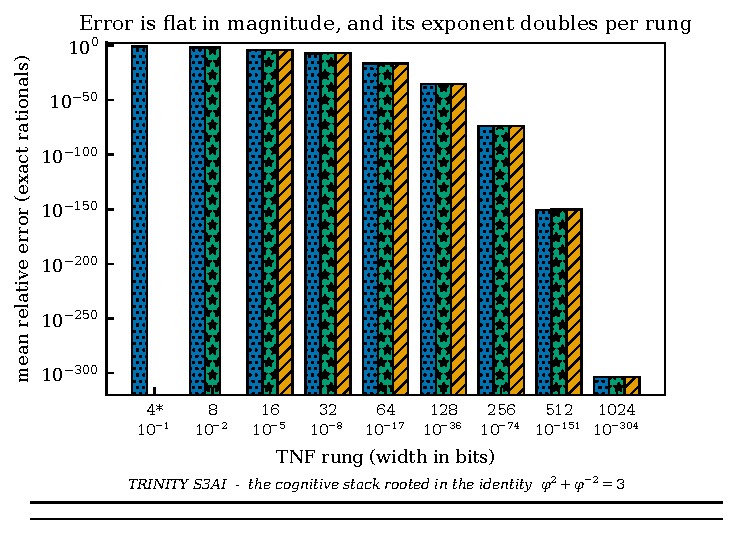
\includegraphics[width=0.86\textwidth]{tnf_ladder_acc.pdf}
\caption{The same data. Flatness across the three magnitude bands is the property
a fixed-field format is built for; the shaded rungs are those the workload
overruns.}
\label{fig:ladderacc}
\end{figure}


\begin{figure}[t]\centering
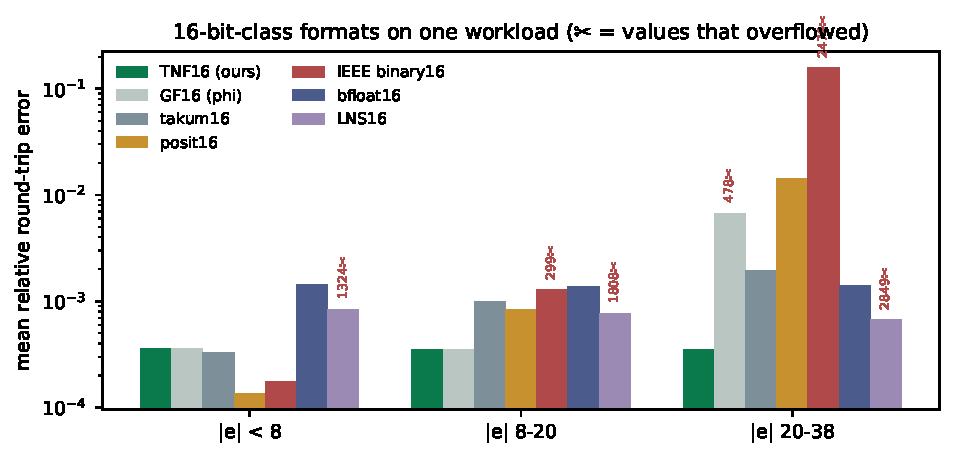
\includegraphics[width=0.92\textwidth]{tnf_competition.pdf}
\caption{The same data. Scissors mark values that overflowed.}
\label{fig:field}
\end{figure}

Three readings, including the one that goes against us.

\paragraph{TNF16 is flat, and alone in being flat without clipping.} Its error
is $3.5\mathrm{e}{-4}$ at every magnitude in the workload and it discards
nothing. bfloat16 is also flat and clip-free, at roughly four times the error.
Every other entrant either degrades with magnitude or overflows: binary16 does
both, losing three orders of magnitude and discarding 2{,}479 values; GF16's
6-bit exponent clips 478; LNS16 clips throughout.

\paragraph{At 32 bits the binary formats win outright.} Running the same
workload on the 32-bit class: GF32 is flat at $3.4\mathrm{e}{-7}$ with no
clipping, but IEEE binary32 is flat at $2.1\mathrm{e}{-8}$, and posit32 and
takum32 are better still near unity ($2.1\mathrm{e}{-9}$ and
$4.9\mathrm{e}{-9}$). Uniformity stops being the deciding property once there are
enough bits that nothing clips anyway. The TNF argument is a 16-bit-class
argument, and we do not extend it.

\paragraph{Near unity we lose.} posit16 at $1.36\mathrm{e}{-4}$ and binary16 at
$1.76\mathrm{e}{-4}$ are more accurate than TNF16 there, by a factor of two and
a half and of two. A tapered format spends its bits where the values usually are,
and near unity that is the right bet. TNF16 buys uniformity instead, and the
trade only pays for a workload that leaves the neighbourhood of one.

\paragraph{takum16 and tekum16 are the same format here, exhaustively.} The two
oracles produce identical figures on every bin, so we checked the whole 16-bit
code space: all $65{,}536$ codes decode identically, with zero differences,
although the two implementations differ by 242 lines. The reconstruction our
tekum oracle implements \emph{is} takum16. Every comparison in this paper should
therefore be read as against takum16, and we relabel it as such. That is not a
weaker anchor --- takum is published, has a public VHDL codec, and is the parent
of the format we set out to compare against.

\section{Hardware}\label{sec:hardware}

Synthesis with Yosys~0.65~\cite{yosys}, place and route with
nextpnr-xilinx~(1743d0f)~\cite{nextpnr} on a
Xilinx XC7A200T, hard multipliers disabled so the figures describe fabric alone.
Bitstream generation uses Project X-Ray. No vendor tool is involved at any step,
which is what makes the numbers checkable by a reader without a licence.

\begin{table}[t]\centering
\caption{TNF multiplier, post-route, one harness across the whole lineup so the
rows are comparable. Latency one cycle, throughput one result per cycle.}
\label{tab:ladder}
\begin{tabular}{lrrr}
\toprule
rung & LUTs & DSP48 & $F_{\max}$ \\
\midrule
TNF4  & $12$      & $0$ & $161.11$\,MHz \\
TNF8  & $50$      & $0$ & $153.23$\,MHz \\
TNF16 & $212$     & $0$ & $131.73$\,MHz \\
TNF32  & $1{,}477$  & $0$ & $83.27$\,MHz \\
TNF64  & $6{,}140$  & $0$ & $53.26$\,MHz \\
TNF128 & $10{,}029$ & $0$ & $33.23$\,MHz \\
\bottomrule
\end{tabular}
\end{table}

\begin{table}[t]\centering
\caption{The specified ladder. $E_t$ is the trit budget, $M$ the mantissa width,
range in decades. Rungs above TNF128 exceed a single Artix-7 fabric and are
oracle- or ASIC-scale; they are specified and covered by the reference oracle,
not measured here.}
\label{tab:spec}
\begin{tabular}{lrrr@{\hskip 2em}lrrr}
\toprule
rung & $E_t$ & $M$ & decades & rung & $E_t$ & $M$ & decades \\
\midrule
TNF4  & $2$ & $1$  & $2.4$ & TNF64   & $7$  & $52$   & $658$ \\
TNF8  & $3$ & $4$  & $8$   & TNF128  & $8$  & $115$  & $1{,}975$ \\
TNF16 & $4$ & $9$  & $24$  & TNF256  & $9$  & $242$  & $5{,}925$ \\
TNF32 & $6$ & $25$ & $73$  & TNF512  & $10$ & $497$  & $17{,}775$ \\
       &     &      &       & TNF1024 & $11$ & $1006$ & $53{,}326$ \\
\bottomrule
\end{tabular}
\end{table}

\begin{figure}[t]\centering
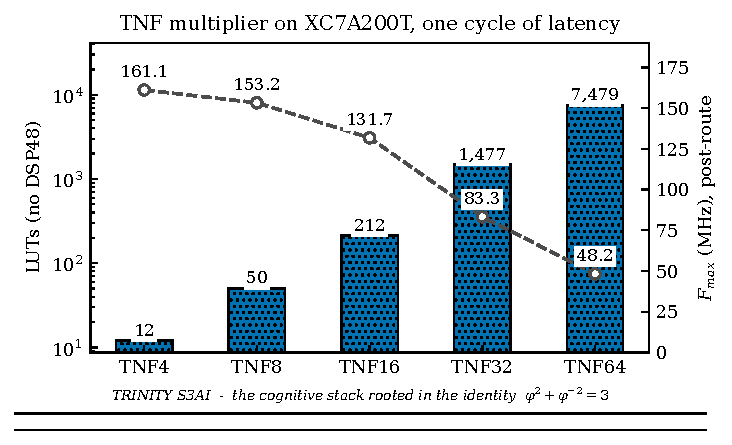
\includegraphics[width=0.82\textwidth]{tnf_ladder.pdf}
\caption{Area and achieved frequency across the ladder.}
\label{fig:ladder}
\end{figure}

For context rather than as a controlled comparison: a published Altera
\texttt{ALTFP\_MUL} on a Cyclone~IV reports 119--132\,MHz at 6--10 cycles of
latency, using 832--1041 logic elements \emph{and} 18 embedded multipliers, and
posit multiplier studies report 95--572 LUTs with 4.28--15.55\,ns of logic delay.
Different devices and different toolchains; we draw no equivalence from them
beyond the observation that TNF16's figures sit inside that envelope on all four
axes at once, on a fabric that gives the format no ternary advantage.

Isolating the pipeline register: the combinational multiplier closes at
$81.35$\,MHz, the two-stage version at $147.32$\,MHz. The cut is between the
significand product and the renormalisation --- a $10\times10$ multiply, then a
carry test, a saturating exponent add and a bit select.

\section{Two width defects, and why they generalise}\label{sec:width}

Section~\ref{sec:hardware} reports what the datapath costs once every bus is
derived from the format's own parameters. It was not measured that way first.
The two defects below --- one of area, one of correctness --- are the same
mistake, a width chosen by hand, and they are reported because that mistake is
not specific to TNF.

\subsection{Interface width dominated the arithmetic}

Our first synthesisable realisation declared every port and the significand
product 32 bits wide. Nothing in TNF16 is 32 bits: the mantissa field is 9, so
$1{+}M$ is 10 and their product is exactly 20; the exponent offset never exceeds
$\mathrm{OFFSET\_MAX}=80$, which is 7. Synthesis built a $32\times32$ multiplier
and a 32-bit comparison tree and charged for it (Figure~\ref{fig:width}):
1{,}179 LUTs, or three DSP48 blocks, against 219 LUTs and none once the buses
match the values they carry. The arithmetic is unchanged.

\begin{figure}[t]\centering
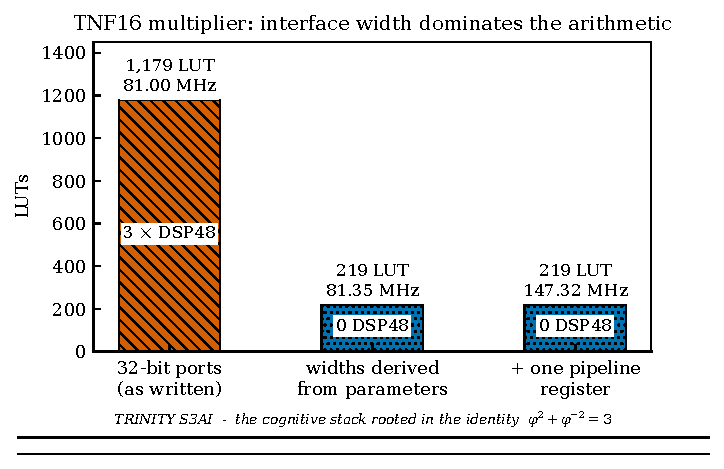
\includegraphics[width=0.82\textwidth]{tnf_width.pdf}
\caption{The same arithmetic at three interface widths.}
\label{fig:width}
\end{figure}

\subsection{The same width decided correctness}

At TNF32 the significand product needs 52 bits. The 32-bit wire truncates, and
the module returns wrong results while appearing to support the rung, since its
own documentation names TNF32 as a supported configuration. Measured against a
64-bit reference: 1{,}995{,}730 mismatches in 2{,}128{,}964 combinations.

Deriving every width from the format parameters removes both problems at once. We
report this because the pattern is not specific to TNF: in a parametric
arithmetic core, a width that is merely \emph{large enough for the configuration
that was tested} is a silent-truncation trap at the next one, and it will not be
caught by a testbench written against the tested configuration.

\section{Equivalence}\label{sec:equiv}

Every change above is a claim that timing or width changed and arithmetic did
not. Each was checked rather than argued.

\begin{table}[t]\centering
\caption{Equivalence evidence. The reference for each rung is the module already
trusted for that rung.}
\label{tab:equiv}
\begin{tabular}{lrr}
\toprule
check & combinations / cycles & mismatches \\
\midrule
width-derived vs original, TNF16 (sweep)      & $321{,}156$   & $0$ \\
width-derived vs original, TNF4               & $374$         & $0$ \\
width-derived vs original, TNF8               & $3{,}716$     & $0$ \\
width-derived vs original, TNF16              & $77{,}444$    & $0$ \\
width-derived vs 64-bit reference, TNF32      & $300{,}000$   & $0$ \\
pipelined vs combinational                     & $199{,}994$   & $0$ \\
\midrule
original 32-bit module vs 64-bit ref, TNF32   & $2{,}128{,}964$ & $1{,}995{,}730$ \\
\bottomrule
\end{tabular}
\end{table}

The TNF16 sweep is exhaustive in the sense that matters here: the mantissa space
is covered in full at offset pairs exercising underflow, mid-range and
saturation, then the offsets are covered in full at mantissas that do and do not
carry --- every path through the carry, the saturation and the underflow clamp.
The last row is the point of the section: the width-derived module agrees with
the reference that is correct and disagrees with the one that truncates.


\section{What the law says about improving the ladder}\label{sec:design}

Theorem~\ref{thm:law} makes the design space arithmetic rather than a matter of
taste. Error scales as $2^{-(M+1)}$ and range as $3^{E_t}$, so at a fixed width
the only decision is how many bits the exponent field is allowed to consume ---
and that is decided by how efficiently $3^{E_t}$ values pack into
$\lceil E_t \log_2 3\rceil$ bits.

\begin{table}[t]\centering
\caption{Packing efficiency of the exponent field. The theoretical floor is
$\log_2 3 = 1.585$ bits per trit.}
\label{tab:pack}
\begin{tabular}{rrrrr}
\toprule
$E_t$ & values $3^{E_t}$ & bits & capacity & efficiency \\
\midrule
$3$  & $27$    & $5$  & $32$   & $84.4\%$ \\
$\mathbf{4}$  & $81$    & $7$  & $128$  & $\mathbf{63.3\%}$ \\
$5$  & $243$   & $8$  & $256$  & $\mathbf{94.9\%}$ \\
$6$  & $729$   & $10$ & $1024$ & $71.2\%$ \\
$\mathbf{7}$  & $2187$  & $12$ & $4096$ & $\mathbf{53.4\%}$ \\
$8$  & $6561$  & $13$ & $8192$ & $80.1\%$ \\
$10$ & $59049$ & $16$ & $65536$ & $90.1\%$ \\
\bottomrule
\end{tabular}
\end{table}

\paragraph{The width convention counts positions, and one rung breaks it.}
A rung's width is its position count with a trit occupying one position, so the
layout is $1 + E_t + M = N$. Three of the four specified rungs satisfy it exactly:
TNF4 is $1+2+1$, TNF8 is $1+3+4$, TNF32 is $1+6+25$. TNF16 is
$1+4+9 = 14$, two positions short of its name, and neither specification file
gives a reason. The likely history is visible in the parameters: TNF16 inherits
GF16's $\varphi$-optimal $M = 9$ and replaces GF16's six-bit exponent with four
trits, which buys range --- $3^4 = 81$ steps against $2^6 = 64$ --- and frees two
positions that were never re-spent. It is the one rung derived from its parent
rather than from the width rule.

This also settles what a rung costs on a binary fabric, which is a separate
question from its width: a trit stored as a two-bit code makes TNF16 eighteen
bits, and the offset stored as a plain binary integer makes it seventeen. Those
are fabric costs, not format widths, and confusing the two is what made the
ladder appear not to fit.

\paragraph{The slack is not confined to one rung.} Applying $1 + E_t + M = N$ to
every specified rung separates the two documents that define the ladder. The four
rungs of the machine-readable specification obey it at TNF4, TNF8 and TNF32;
the five upper rungs, which exist only in a research note, miss it by four to six
positions each, and the note and the specification disagree with each other about
TNF32.

\begin{table}[t]\centering
\caption{The width rule across the ladder. $k$ is the shortfall
$N - (1 + E_t + M)$. The reconciled column is $M = N - 1 - E_t$, which changes
nothing at the three rungs that already obey the rule.}
\label{tab:ladder-sweep}
\begin{tabular}{lrrrrrr}
\toprule
rung & source & $E_t$ & $M$ & $1{+}E_t{+}M$ & $k$ & reconciled $M$ \\
\midrule
TNF4    & spec & $2$  & $1$    & $4$    & $0$ & $1$ \\
TNF8    & spec & $3$  & $4$    & $8$    & $0$ & $4$ \\
TNF16   & spec & $4$  & $9$    & $14$   & $2$ & $\mathbf{11}$ \\
TNF32   & spec & $6$  & $25$   & $32$   & $0$ & $25$ \\
TNF32   & note & $5$  & $21$   & $27$   & $5$ & --- \\
TNF64   & note & $7$  & $52$   & $60$   & $4$ & $\mathbf{56}$ \\
TNF128  & note & $8$  & $115$  & $124$  & $4$ & $\mathbf{119}$ \\
TNF256  & note & $9$  & $242$  & $252$  & $4$ & $\mathbf{246}$ \\
TNF512  & note & $10$ & $497$  & $508$  & $4$ & $\mathbf{501}$ \\
TNF1024 & note & $11$ & $1006$ & $1018$ & $6$ & $\mathbf{1012}$ \\
\bottomrule
\end{tabular}
\end{table}

No single alternative convention explains the upper rungs either: reading the
exponent as $\lfloor E_t\log_2 3\rfloor$ bits fits TNF16, TNF64, TNF128 and
TNF1024 exactly but overshoots TNF256 and TNF512 by one and misses TNF32
entirely. We conclude that the upper ladder was tabulated rung by rung rather than
derived, and that reconciling it costs nothing at the rungs that are already
right.

\paragraph{What the two free positions were worth, and where they went.} Because
the exponent cancels in Theorem~\ref{thm:law}, the menu at sixteen positions could
be read off before measuring, and the measurement confirmed it to four significant
figures:

\begin{table}[t]\centering
\caption{The three ways to spend TNF16's two unallocated positions. Error and
range trade against each other exactly as Theorem~\ref{thm:law} predicts; nothing
in any row is worse than the unfilled rung.}
\label{tab:tnf16-fill}
\begin{tabular}{lrrrr}
\toprule
variant & positions & mean rel.\ error & decades & vs.\ takum16 (far) \\
\midrule
unfilled, $E_t{=}4$, $M{=}9$  & $14$ & $3.37\mathrm{e}{-4}$ & $24$  & $5.46\times$ \\
$\mathbf{E_t{=}4}$, $\mathbf{M{=}11}$ (adopted) & $\mathbf{16}$ & $\mathbf{8.63\mathrm{e}{-5}}$ & $24$ & $\mathbf{22.68\times}$ \\
$E_t{=}5$, $M{=}10$           & $16$ & $1.69\mathrm{e}{-4}$ & $73$  & --- \\
$E_t{=}6$, $M{=}9$            & $16$ & $3.37\mathrm{e}{-4}$ & $\mathbf{219}$ & --- \\
\bottomrule
\end{tabular}
\end{table}

The last row is the law's own consistency check: adding two trits of exponent
while holding $M$ leaves the error bit-identical and multiplies the range
ninefold.

\paragraph{The positions were spent on mantissa, and the reason is a measurement.}
Corollary~\ref{cor:three} forbids recommending a budget without naming a workload,
so we named one. At the 16-bit class the extra range is not consumed:
quantised-inference tensors span roughly $2^{-14}$ to $2^{14}$, and $E_t = 4$
already clips nothing at $\pm 40$ binades --- zero clips in 2000 values. $E_t = 6$
would have bought $\pm 364$ binades at bit-identical error, which is range nobody
spends at sixteen bits. So $M = 11$: the error falls by exactly $4.00$, and
against takum16 the rung moves from $0.92\times / 2.88\times / 5.49\times$ to
$3.70\times / 11.21\times / 22.68\times$, no longer losing the near bin. In
silicon it costs $443$ LUTs against $372$, a $19\%$ increase, at $136.44$\,MHz
against $131.73$ --- no frequency penalty.

All three ratios in this section and in Figure~\ref{fig:acc} come from one
script, \texttt{gen\_figures.py}, which computes them from the oracles at seed
$20260809$ rather than transcribing them. They were hardcoded until 2026-08-09 and
had drifted: the figure still carried $M = 9$ and the label \texttt{tekum16} after
the rung moved and the oracle was shown to decode identically to takum. A figure
that disagrees with the table it illustrates is the same defect class as a gate
that cannot go red.

Conformance was re-run in full rather than assumed: round-trip with sign
2000/2000, encoding monotone with zero inversions, $\pm$ symmetry with zero
mismatches in 500, both range boundaries decoding. A \texttt{width\_rule} test now
asserts $1 + E_t + M = N$ in the specification itself, so the position count is
checked rather than remembered. All nine rungs satisfy it.

\section{Why ternary, and exactly how much}\label{sec:whyternary}

The case for a ternary exponent is usually made by citing radix economy and left
there. We state it, then bound it in two directions --- what a binary fabric takes
back, and what the radix of the \emph{scale} is worth as distinct from the radix
of the \emph{exponent} --- because both bounds turn out to be decisive for the
design and neither is folklore.

\begin{theorem}[Radix economy]
\label{thm:economy}
Representing $R$ distinct values in radix $b$ costs $b\log_b R = b\ln R/\ln b$
state-slots. The factor $b/\ln b$ is minimised at $b = e$; among integers it is
$3/\ln 3 = 2.731$ against $2/\ln 2 = 2.885$, so a ternary field is $5.3\%$ more
economical than a binary one.
\end{theorem}

This is the classical argument~\cite{hayes2001,radixeconomy} and it is what
motivates a ternary exponent. It is also stated in a currency --- state-slots ---
that no binary fabric pays in. The next theorem says what happens when it does.

\begin{theorem}[No free range on a binary fabric]
\label{thm:nofree}
An exponent field of $E_t$ trits spans $3^{E_t}$ values. Stored as a binary
integer it occupies $\lceil E_t\log_2 3\rceil$ bits, a field spanning
$2^{\lceil E_t\log_2 3\rceil} \geq 3^{E_t}$ values. Hence on a binary fabric a
ternary exponent never spans more values per bit than a binary one, with equality
only at $E_t = 0$. Writing $\rho(E_t) = 3^{E_t}/2^{\lceil E_t\log_2 3\rceil}$ for
the utilisation, $\rho \in (1/2, 1]$ and $\rho$ does not converge.
\end{theorem}

\begin{table}[t]\centering
\caption{Utilisation $\rho(E_t)$ of the binary field holding an $E_t$-trit
exponent. The ladder's present budgets, $E_t \in \{4, 7\}$, are the two worst
entries in the range.}
\label{tab:rho}
\begin{tabular}{lrrrrrrrrrr}
\toprule
$E_t$ & 2 & 3 & 4 & 5 & 6 & 7 & 8 & 9 & 10 & 11 \\
\midrule
$\rho$ & $56.2$ & $84.4$ & $\mathbf{63.3}$ & $94.9$ & $71.2$ & $\mathbf{53.4}$ & $80.1$ & $60.1$ & $90.1$ & $67.6$ \\
\bottomrule
\end{tabular}
\end{table}

Run as an optimisation rather than an inequality, the same statement is sharper
than it looks. Asking which exponent encoding a binary fabric prefers at
$(N, R) = (16, 24)$, $(32, 219)$ and $(64, 658)$ returns the same mantissa width
for both --- $M = 10$, $23$ and $53$ respectively. The ternary encoding does not
lose on a binary fabric; at these widths the ceilings absorb the difference and it
exactly ties, which is the strongest form of ``never more values per bit''.

Theorem~\ref{thm:nofree} is the reason the ladder's rung widths must be read as
position counts and not bit counts, and it is where our own first reading of the
ladder went wrong: measuring what a trit costs when packed into bits and calling
the result the format's width confuses a fabric cost with a format property. The
independently published balanced-ternary float Ternary27~\cite{ternary27} counts
the same way --- 2 type trits, 1 sign trit, 5 exponent trits and 19 significand
trits, exactly 27 --- which is external corroboration that position counting is
the convention in this family rather than a reading of our own.

\begin{theorem}[Unallocated positions are a pure loss]
\label{thm:alloc}
Let a rung of $N$ positions carry a sign, $E_t$ exponent trits and $M$ mantissa
bits with $1 + E_t + M = N - k$, $k \geq 0$. Then relative to the rung with the
same $E_t$ and $M + k$, its expected relative error is larger by exactly $2^{k}$
and its dynamic range is identical.
\end{theorem}

\begin{proof}
By Theorem~\ref{thm:law} the expected relative error is
$\tfrac12 \mathbb{E}[1/s]\,2^{-(M+1)}$, in which the exponent does not appear;
replacing $M$ by $M+k$ multiplies it by $2^{-k}$. The dynamic range is
$3^{E_t}$ binades, a function of $E_t$ alone, so it is unchanged. Nothing else in
the layout depends on $M$. \qed
\end{proof}

Theorem~\ref{thm:alloc} converts the slack of Section~\ref{sec:design} into a
number without any measurement, and the measurement then confirms it. Against a
workload built in exact arithmetic --- necessary above TNF32, where a
double-precision probe measures its own resolution rather than the format's ---
the predicted and observed factors are:

\begin{table}[t]\centering
\caption{Unallocated positions per rung, the loss Theorem~\ref{thm:alloc}
predicts, and the loss measured against the reconciled rung
$M = N - 1 - E_t$. Exact-arithmetic workload, 800 probes per rung.}
\label{tab:alloc}
\begin{tabular}{lrrrr}
\toprule
rung & $k$ & predicted & measured \\
\midrule
TNF16  & $2$ & $4\times$  & $4.03\times$  \\
TNF64  & $4$ & $16\times$ & $15.43\times$ \\
TNF128 & $4$ & $16\times$ & $15.99\times$ \\
TNF256 & $4$ & $16\times$ & $15.24\times$ \\
\bottomrule
\end{tabular}
\end{table}

The final question is one the ladder answers implicitly and, as far as we can
find, no one has stated: TNF encodes its exponent in radix 3 but scales by
$2^{e}$, whereas Ternary27 scales by $3^{e}$. These are different choices and
they are separable.

\begin{theorem}[The scale radix, and why 2 beats 3]
\label{thm:scaleradix}
Let a format scale by $r^{e}$ with a normalised significand uniformly quantised
over $[1, r)$ by $M$ bits. Then its expected relative error on a log-uniform
workload is $\kappa(r)\,2^{-M}$ with
\[
\kappa(r) \;=\; \frac{(r-1)^{2}}{r\ln r},
\qquad \kappa(2) = 0.72135,\quad \kappa(3) = 1.21365 .
\]
Holding the field layout fixed, moving the scale from $r=2$ to $r=3$ therefore
multiplies the error by $\kappa(3)/\kappa(2) = 1.6825$ while multiplying the
dynamic range by $\log_2 3 = 1.5850$. Measured in positions, it costs
$\log_2 1.6825 = 0.7506$ of precision and buys $\log_3 1.5850 = 0.4192$ of range:
a net loss of $0.3314$ positions per number. A power-of-two scale strictly
dominates a power-of-three scale at equal width.
\end{theorem}

\begin{proof}
The quantisation step over $[1,r)$ is $(r-1)2^{-M}$ and the mean absolute
rounding error is half of it. On a log-uniform workload the significand has
density $1/(s\ln r)$ on $[1,r)$, so
$\mathbb{E}[1/s] = \frac{1}{\ln r}\int_1^{r} s^{-2}\,ds = \frac{1-1/r}{\ln r}$.
Multiplying gives $\tfrac12 (r-1)2^{-M}\cdot\frac{1-1/r}{\ln r}$, and
$\tfrac12(r-1)(1-1/r) = (r-1)^2/2r$. Absorbing the factor $\tfrac12$ into the
$2^{-(M+1)}$ convention of Theorem~\ref{thm:law} yields $\kappa$ as stated. For
the range, $E_t$ trits span $3^{E_t}$ steps of $\log_2 r$ binades each. One
mantissa bit halves the error and one exponent trit triples the range, which
fixes the exchange rate between the two currencies and gives the position
figures. \qed
\end{proof}

Direct measurement at two rungs, encoding and decoding through both scales in
exact arithmetic, gives error ratios of $1.675$ at $(E_t,M) = (4,11)$ and $1.690$
at $(6,25)$ against the predicted $1.6825$, and range ratios of $1.583$ and
$1.585$ against the predicted $1.5850$.

\begin{corollary}[What TNF is, precisely]
TNF is not a ternary float in the sense of Ternary27; it is a binary-radix float
whose exponent is \emph{encoded} in balanced ternary. Theorem~\ref{thm:scaleradix}
says that this is the better of the two available choices by $0.331$ positions per
number, and Theorem~\ref{thm:nofree} says that the ternary encoding pays only on a
ternary fabric. The two together delimit the format exactly: the radix choice is
right on any fabric, and the encoding choice is right on one.
\end{corollary}


\section{The regime field is a universal code}
\label{sec:codes}

Theorem~\ref{thm:dichotomy} identifies the exponent's encoding as a prefix code.
That identification is worth making explicit, because it places the taxonomy of
Section~\ref{sec:taxonomy} inside a hierarchy that predates every format in the
catalogue by decades~\cite{elias1975}.

\begin{theorem}[The staircase is the codeword-length function]
\label{thm:code}
Let a format of $N$ positions encode its exponent with a prefix code assigning
$e$ a codeword of length $\ell(e)$. Then
$M_{\mathrm{eff}}(e) = N - 1 - \ell(e)$, and the staircase form is the growth
rate of $\ell$ and nothing else.
\end{theorem}

The catalogue's three tapering classes are then three points in the classical
hierarchy: a unary regime, $\ell \propto |e|$, gives posit's arithmetic
staircase; a length-prefixed binary regime, $\ell \propto \log_2|e|$, gives
takum's geometric one; a fixed field, $\ell = \mathrm{const}$, gives no staircase
at the price of bounded support. Elias' $\gamma$, $\delta$ and $\omega$ codes
occupy the logarithmic class at successively finer asymptotics.

\begin{theorem}[Logarithmic is the floor]
\label{thm:floor}
For any prefix code on the integers, $\ell(e) \geq \log_2|e|$ for infinitely many
$e$. Hence no format of unbounded range tapers more gently than one bit per
doubling of $|e|$, asymptotically.
\end{theorem}

\begin{proof}
Kraft's inequality gives $\sum_e 2^{-\ell(e)} \leq 1$. If $\ell(e) < \log_2|e|$
for all but finitely many $e$, the tail of the sum exceeds
$\sum_e 1/|e|$, which diverges. \qed
\end{proof}

Theorem~\ref{thm:floor} is worth stating plainly because it bounds this work as
much as its competitors: takum's regime is asymptotically optimal, and no format
--- TNF included --- can beat it over unbounded range. What TNF does instead is
decline the unbounded range, which Theorem~\ref{thm:dichotomy} shows is the only
other option. The measured advantages of Section~\ref{sec:accuracy} are therefore
advantages \emph{inside TNF's range}, which is where the taper has already cost
takum the bits, and they should never be read as a claim beyond it.

\begin{theorem}[The regime's radix does not matter]
\label{thm:radixinv}
A regime spending one digit per multiplication of $|e|$ by $r$, over an alphabet
of $r$ symbols, costs $\log_2 r \cdot \log_r |e| = \log_2 |e|$ bits, independent
of $r$. The staircase form is invariant to the regime's radix.
\end{theorem}

Theorem~\ref{thm:radixinv} retracts a construction we proposed in an earlier draft
of this work. Having observed the gap between the arithmetic and geometric
classes, we suggested a regime spending one trit per tripling of $|e|$ as the
natural way for a ternary format to occupy it. It does not occupy it: building
both codes and normalising each to satisfy Kraft, the two codeword-length
functions differ by an additive constant of exactly $1$ at every $|e|$ from $1$ to
$4096$. One trit per tripling is takum's staircase with a different constant, not
a third form. A ternary fabric changes what the regime costs to decode; it does
not change what it costs to encode.

\paragraph{The gap is real, occupiable, and empty for a reason we can only
conjecture.} Growth rates strictly between $\log_2|e|$ and $|e|$ do exist and are
Kraft-feasible --- $\ell(e) = \lceil\sqrt{|e|}\rceil$ is one --- and such a code
is not dominated. At $N = 16$, normalised so that all three are legal prefix
codes:

\begin{table}[t]\centering
\caption{$M_{\mathrm{eff}}$ by $|e|$ and usable range for three regime codes at
$N = 16$, each normalised to satisfy Kraft. The square-root code is a genuine
Pareto point: more precision than the logarithmic code throughout the core, more
range than the unary one.}
\label{tab:codes}
\begin{tabular}{lrrrrrr}
\toprule
regime & $|e|{=}1$ & $4$ & $16$ & $64$ & $256$ & binades \\
\midrule
unary, $\ell \propto |e|$ (posit class)      & $11$ & $10$ & $7$ & $-5$ & $-53$ & $43$ \\
$\ell = \lceil\sqrt{|e|}\rceil$              & $11$ & $10$ & $8$ & $4$  & $-4$  & $121$ \\
$\ell \propto \log_2|e|$ (takum class)       & $9$  & $7$  & $5$ & $3$  & $1$   & $511$ \\
\bottomrule
\end{tabular}
\end{table}

For reference, a fixed field reaching the same 121 binades as the square-root code
spends 8 bits on the exponent and holds $7$ bits flat everywhere --- better than
the square-root code beyond $|e| \approx 30$ and worse below it, which is the
taper trade in miniature.

So the gap is not empty because its occupants are dominated; they are not. Our
first explanation was decode cost, and building the hardware refutes it.

\subsection{What a regime costs in silicon}\label{sec:regimecost}

We wrote three regime codecs to one interface --- a 16-bit word in, an exponent
and a mantissa shift out, and the mirror encoder --- and synthesised each under a
single harness on XC7A200T with Yosys and nextpnr-xilinx, hard multipliers
disabled. These are structural models of the three classes, not reproductions of
the published posit or takum codecs; what they compare is a run-scanned regime
against a length-prefixed one, which is the structural difference the taxonomy
names.

\begin{table}[t]\centering
\caption{Regime codec cost by class, post-route on XC7A200T under one harness,
no DSP. Figures are net of the harness, which costs $24$ LUTs and was synthesised
separately and subtracted; the round-trip column is decode plus encode.}
\label{tab:regimecost}
\begin{tabular}{lrrrrr}
\toprule
class & \multicolumn{2}{c}{decode} & \multicolumn{2}{c}{encode} & round trip \\
      & LUTs & $F_{\max}$ & LUTs & $F_{\max}$ & LUTs \\
\midrule
unary, $\ell \propto |e|$ (posit)          & $379$ & $36.8$\,MHz  & $59$  & $211.2$\,MHz & $438$ \\
$\ell \propto \log_2|e|$ (takum)           & $\mathbf{6}$ & $\mathbf{805.8}$\,MHz & $\mathbf{34}$ & $\mathbf{285.1}$\,MHz & $\mathbf{40}$ \\
$\ell = \lceil\sqrt{|e|}\rceil$            & $393$ & $33.1$\,MHz  & $123$ & $96.4$\,MHz  & $516$ \\
\midrule
fixed field (GF, TNF)                     & $0$   & ---          & $0$   & ---          & $\mathbf{0}$ \\
\bottomrule
\end{tabular}
\end{table}

The conjecture said the square-root code would be too expensive to be worth
building. It is not: it costs $18\%$ more than the unary regime round trip, and
the unary regime ships in production. What the measurement does show is that the
expense lies somewhere else than we assumed, and this has a closed form.

\begin{theorem}[Decode cost is set by the scan, not by the staircase]
\label{thm:scan}
A regime whose codeword length is delimited by a run must examine up to $N-1$
positions to decode, giving cost $\Theta(N)$. A regime whose length is carried in
a fixed field of $b$ bits requires no scan and a shift of at most $2^{b}-1$,
giving cost $\Theta(1)$ in $N$. The two costs are independent of the growth rate
of $\ell$, and therefore of the staircase form.
\end{theorem}

Theorem~\ref{thm:scan} predicts the table exactly. The unary and square-root codes
share the same 15-position scan and cost $403$ and $417$ LUTs, a difference of
$3.5\%$ that is the squarer and nothing else; the length-prefixed code has no scan
and costs $30$. The square-root code is geometrically intermediate and structurally
identical to the unary one, which is the point: \emph{the staircase form and the
decode cost are independent axes}, and a taxonomy of one does not predict the
other.

\begin{corollary}[The logarithmic regime is not a trade]
\label{cor:takumwins}
Against the unary regime the length-prefixed one is better on every axis measured:
asymptotically optimal by Theorem~\ref{thm:floor}, $11\times$ smaller round trip,
and $22\times$ faster to decode. The published bounded-regime posit
variants~\cite{positgap}, which cap the regime field precisely to avoid the scan,
are the same conclusion reached from the other direction.
\end{corollary}

\begin{corollary}[The measured price of unbounded range]
\label{cor:price}
A fixed field has no regime codec at all. The dichotomy of
Theorem~\ref{thm:dichotomy} therefore has a hardware statement: unbounded range
costs $40$ LUTs at best and $438$ at worst on this device, against $0$ for a
format that declines it. Section~\ref{sec:convert} converts those LUTs into the
same currency as the accuracy results, which is the only way to say whether they
matter.
\end{corollary}

We are left without an explanation for the empty gap. It is not domination, since
the square-root code is Pareto-undominated; and it is not cost, since it is within
$16\%$ of a regime that ships. Both of our explanations are now measured and both
are wrong, and we record that rather than replace it with a third.


\section{Converting silicon into precision}\label{sec:convert}

Corollary~\ref{cor:price} gives a regime's cost in LUTs and Section~\ref{sec:accuracy}
gives an accuracy ratio, and the two cannot be compared until they are in one
currency. They can be: at a fixed class, a mantissa bit has a marginal area, and
by Theorem~\ref{thm:law} it has a known value in accuracy.

\begin{theorem}[Area and precision are commensurable]
\label{thm:convert}
Let $\lambda = \mathrm{d}A/\mathrm{d}M$ be the marginal area of a mantissa bit at
a given class. A regime codec costing $C$ LUTs is then equivalent to $C/\lambda$
mantissa bits of silicon, and by Theorem~\ref{thm:law} to a factor
$2^{C/\lambda}$ in accuracy at equal area.
\end{theorem}

Measuring $\lambda$ directly --- the same width-derived multiplier synthesised at
$M = 7, 9, \ldots, 25$ under one harness --- gives $285$, $372$, $443$, $567$,
$696$, $870$, $1238$ and $1683$ LUTs. The marginal cost is not constant: it rises
from $35.5$ LUTs per bit between $M{=}9$ and $M{=}11$ to $111.2$ between $M{=}21$
and $M{=}25$. Taking the local value at each class, $\lambda = 48.8$ at the
16-bit class and $111.2$ at the 32-bit one:

\begin{table}[t]\centering
\caption{Regime area converted into mantissa bits through
Theorem~\ref{thm:convert}. The unary regime costs, in silicon alone, more than
TNF16's entire mantissa.}
\label{tab:convert}
\begin{tabular}{lrrr}
\toprule
regime & LUTs & bits at 16-bit class & bits at 32-bit class \\
\midrule
unary (posit class)          & $438$ & $\mathbf{8.98}$ & $3.94$ \\
length-prefixed (takum class) & $40$  & $0.82$ & $0.36$ \\
\bottomrule
\end{tabular}
\end{table}


\subsection{How area grows along the ladder}\label{sec:arealaw}

Theorem~\ref{thm:convert} needs $\lambda$, and $\lambda$ is a derivative of an
area law we can state. Fitting $A(M) = cM^{\alpha}$ to the eight rungs from
$M{=}7$ to $M{=}25$ gives $\alpha = 1.406$ at $R^2 = 0.984$, and combined with
Theorem~\ref{thm:law} it predicts a scaling relation:

\begin{proposition}[Error decays as a stretched exponential in area]
\label{prop:stretched}
With $\varepsilon \propto 2^{-M}$ and $A \propto M^{\alpha}$,
$\ln(1/\varepsilon) \propto A^{1/\alpha}$.
\end{proposition}

Measured over $M \in [7,25]$ --- a sixfold range of area and a $250{,}000$-fold
range of error --- the constant of proportionality holds to within $27\%$ and
drifts monotonically downward, so the relation is an approximation and we label
it a proposition rather than a theorem. The drift has a cause, and finding it
falsified a prediction we registered before synthesising.

\paragraph{The exponent is not constant, and the fit does not extrapolate.} We
predicted from the $[7,25]$ fit that the reconciled TNF64, at $M = 56$, would
cost $4{,}762$ LUTs. It costs $7{,}479$ at $48.20$\,MHz --- the prediction is low
by $1.57\times$. Reading $\alpha$ locally rather than globally shows why: it rises
monotonically, from $1.06$ between $M{=}7$ and $M{=}9$ to $1.78$ between $M{=}15$
and $M{=}17$ and $1.85$ between $M{=}25$ and $M{=}56$.

\begin{theorem}[The ladder's area law]
\label{thm:alpha}
A rung's area is a fixed overhead --- registers, the exponent adder, the
renormalisation --- plus a significand multiplier quadratic in $M$:
\[
A(M) \;=\; f + cM^{2}.
\]
Consequently the effective power-law exponent
$\alpha(M) = \mathrm{d}\ln A/\mathrm{d}\ln M$ is not a constant but rises
monotonically toward $2$, and the marginal cost of a mantissa bit,
$\lambda = \mathrm{d}A/\mathrm{d}M = 2cM$, is \emph{linear} in $M$ rather than
fixed.
\end{theorem}

Synthesising the same width-derived multiplier at fourteen mantissa widths from
$M{=}7$ to $M{=}90$ --- $285$, $372$, $443$, $567$, $696$, $870$, $1238$, $1683$,
$2601$, $3990$, $5934$, $7479$, $12232$ and $19980$ LUTs --- and fitting both
parameters gives $f = 141$ LUTs and $c = 2.4455$ LUTs per bit squared at
$R^2 = 0.99963$, with a maximum deviation of $9.9\%$ across a seventyfold range of
area. Read locally, $\alpha$ climbs from $1.06$ between $M{=}7$ and $M{=}9$ to
$2.20$ between $M{=}56$ and $M{=}70$, which is Theorem~\ref{thm:alpha} rather than
noise. On the registered prediction the structural model is right to $+4.4\%$
where the single power law was low by $36.3\%$; we report both, since the power
law was ours and we published the prediction before synthesising.

\begin{theorem}[A regime's worth in precision falls as $1/M$]
\label{thm:oneoverm}
By Theorems~\ref{thm:convert} and~\ref{thm:alpha}, a regime codec of fixed area
$C$ is worth
\[
\frac{C}{\lambda} \;=\; \frac{C}{2cM}
\]
mantissa bits, inversely proportional to the mantissa width. It is worth at least
one mantissa bit exactly while $M \leq C/2c$.
\end{theorem}

\begin{table}[t]\centering
\caption{The same regime codecs valued at five mantissa widths through
Theorem~\ref{thm:oneoverm}, with $c = 2.4455$ measured on XC7A200T. The unary
regime's silicon exceeds an entire TNF16 mantissa; the length-prefixed regime is
below one bit everywhere above the 8-bit class.}
\label{tab:oneoverm}
\begin{tabular}{rrrr}
\toprule
$M$ & $\lambda$ (LUT/bit) & unary, $438$ LUT & length-prefixed, $40$ LUT \\
\midrule
$9$  & $44.0$  & $\mathbf{9.95}$ & $0.91$ \\
$11$ & $53.8$  & $8.14$ & $0.74$ \\
$25$ & $122.3$ & $3.58$ & $0.33$ \\
$56$ & $273.9$ & $1.60$ & $0.15$ \\
$90$ & $440.2$ & $1.00$ & $0.09$ \\
\bottomrule
\end{tabular}
\end{table}

\begin{corollary}[Break-even widths]
\label{cor:breakeven}
With $c = 2.4455$, the unary regime is worth at least one mantissa bit of silicon
up to $M = 89.6$ --- that is, through the entire 128-bit class --- while the
length-prefixed regime reaches one bit only up to $M = 8.2$. takum's regime
therefore costs less than a single mantissa bit of silicon at every rung above
TNF8, and posit's costs more than one at every rung below TNF256.
\end{corollary}

Corollary~\ref{cor:breakeven} is the exact form of what
Corollary~\ref{cor:narrow} below could only say qualitatively, and it is the sharpest
statement we can make about where a fixed field pays for itself in area: against
posit, almost everywhere; against takum, only at the very bottom of the ladder.

\begin{corollary}[Range is paid for three times, and they are commensurable]
\label{cor:three}
A tapered format pays for unbounded range in three currencies: word positions,
in the regime field; silicon, in the codec; and precision at the extremes, in the
taper. Theorem~\ref{thm:convert} and Theorem~\ref{thm:law} put all three in
mantissa bits, so they can be added.
\end{corollary}

Applied honestly, Corollary~\ref{cor:three} separates the two tapered families
rather than lumping them. Against posit the silicon term alone is $8.98$ bits at
the 16-bit class --- more than TNF16's entire $9$-bit mantissa, so the area a
posit implementation spends decoding its regime would, spent on significand
instead, roughly double the precision budget of a fixed-field format at the same
class. Against takum the silicon term is $0.82$ bits, which is small. The
length-prefixed regime is cheap, and any argument for a fixed field made on area
grounds is an argument against posit and not against takum. Against takum what
remains is the accuracy result of Section~\ref{sec:accuracy}, bounded as
Theorem~\ref{thm:floor} requires to TNF's own range.

\begin{corollary}[The area argument is a narrow-width argument]
\label{cor:narrow}
Since $\lambda$ grows superlinearly in $M$ while a regime codec's cost is roughly
fixed, the same codec converts to fewer mantissa bits as the class widens:
$8.98$ bits at 16 becomes $3.94$ at 32 for the unary regime. The fixed-field area
advantage is therefore strongest where the words are narrowest, which is the
regime in which quantised inference operates and not the one in which numerical
linear algebra does.
\end{corollary}


\section{The value law costs more than the field layout}
\label{sec:valuelaw}

Sections~\ref{sec:regimecost} and~\ref{sec:convert} priced the regime as a field
to be extracted, and synthesising the published decoders shows that this is the
smaller half of the question. We take the takum and posit decoders from an
existing open verification suite --- Verilog, golden-checked against an mpmath
oracle --- and put them through the same harness on XC7A200T.

\begin{table}[t]\centering
\caption{Published 32-bit decoders, post-route on XC7A200T under one harness, no
DSP, converting to binary32. These are the real codecs rather than the structural
models of Table~\ref{tab:regimecost}.}
\label{tab:realcodecs}
\begin{tabular}{lrrrl}
\toprule
decoder & LUTs & RAMB36 & $F_{\max}$ & what dominates \\
\midrule
\texttt{posit32\_decode} & $480$ & $0$ & $49.0$\,MHz & leading-zero count, shift \\
\texttt{takum32\_decode}, published & $76{,}821$ & $0$ & --- & $2^{f}$ table, in logic \\
\texttt{takum32\_decode}, clocked & $10{,}967$ & $\mathbf{84}$ & $11.4$\,MHz & same table, in BRAM \\
TNF32, exponent path & $0$ & $0$ & --- & field read directly \\
\bottomrule
\end{tabular}
\end{table}

The takum row is given twice because one number alone would mislead. Its decoder
evaluates $2^{f_{\mathrm{hi}}/2^{16}}$ from a $65536 \times 48$-bit table, then
applies a Taylor correction through a $108$-bit and an $80$-bit multiply. As
published the table read is combinational, which no synthesiser can map to block
memory, so it was built from logic at $76{,}821$ LUTs. Registering that read and
marking it \texttt{ram\_style="block"} --- one cycle of added latency, and a
pipelined variant of the published module rather than the module itself --- puts
the table where it belongs: $10{,}967$ LUTs and $84$ RAMB36 tiles, which is
$3.1$\,Mbit and $23\%$ of this device's entire block memory. We predicted $85$
tiles from the table geometry before synthesising and measured $84$. Neither
number is a property of takum the format; both are properties of decoding a
logarithmic value law into a linear datapath, and neither is the regime field.

\begin{theorem}[Linear and logarithmic value laws]
\label{thm:valuelaw}
Let a format's value law be $v = s \cdot 2^{e}$ with $s$ and $e$ read from fields
(\emph{linear}), or $v = \pm 2^{\ell}$ for a decoded real $\ell$
(\emph{logarithmic}). A linear law decodes with a shift, cost independent of the
mantissa width. A logarithmic law requires evaluating an exponential, whose cost
is a table or an iterative kernel and is independent of the field layout ---
therefore independent of the staircase form of Section~\ref{sec:taxonomy}.
\end{theorem}

Theorem~\ref{thm:valuelaw} is a second axis, orthogonal to the first. The
staircase taxonomy classifies how a format spends \emph{precision}; the value law
classifies what it costs to \emph{read}. posit is tapered and linear; takum is
tapered and logarithmic; LNS is untapered and logarithmic; GF, TNF and IEEE are
untapered and linear. The two axes are independent, and our earlier reading ---
that decode cost is set by whether the regime is scanned
(Theorem~\ref{thm:scan}) --- describes only the field-extraction term. It remains
correct within that term, and Table~\ref{tab:realcodecs} shows the term is not
where the money is for a logarithmic format.


\begin{theorem}[The logarithmic decode costs by target precision, not by source width]
\label{thm:targetprec}
A $2^{k}$-entry table for $2^{f}$ with a degree-$d$ Taylor correction delivers
\[
P(k,d) \;=\; (d+1)\Bigl(k + \log_2\tfrac{1}{\ln 2}\Bigr) + \log_2 (d+1)!
\]
bits of relative accuracy, so the table is $P \cdot 2^{k}$ bits with
$k = \frac{P - \log_2 (d+1)!}{d+1} - \log_2\frac{1}{\ln 2}$: exponential in the
target precision, reducible only by raising the polynomial degree, which trades
memory for multipliers. The width of the source format does not enter.
\end{theorem}

\begin{proof}
The residual after the table lookup is $x = f_{\mathrm{lo}}\ln 2$ with
$f_{\mathrm{lo}} < 2^{-k}$, and the degree-$d$ Taylor remainder of $e^{x}$ is
$x^{d+1}/(d+1)!$. Taking $-\log_2$ gives the stated $P$. \qed
\end{proof}

Evaluated against direct simulation of the scheme --- the table, the residual and
the polynomial, in exact arithmetic --- the formula holds to $\pm 0.1$ bit at every
point of a $k \in \{4,8,12,16,20\}$ by $d \in \{1,2,3,4\}$ grid, up to the
$51$-bit resolution of the measurement itself.

Theorem~\ref{thm:targetprec} is falsifiable against the suite and survives. The
takum32 decoder carries $d = 2$ and $k = 16$, and $48/3 = 16$ exactly, where 48 is
the table's output width. If the cost were set by the source width, the takum64
decoder would need a larger table; if it is set by the target, it would need the
same one. It reads \texttt{takum32\_2frac.mem} --- \emph{the same file} --- and
emits binary32, as do the takum8, takum16 and takum64 decoders. One table serves
four source widths because all four target one datapath.

\begin{corollary}[The trade curve, and what each target actually costs]
\label{cor:tradecurve}
Theorem~\ref{thm:targetprec} fixes a curve rather than a point, and the cheapest
point on it that fits a given device is a computable quantity. Pricing the $d$
multiplies at $2.4455 P^{2}$ LUTs --- the quadratic term of our own measured area
law, Theorem~\ref{thm:alpha} --- and requiring the table to fit this device's
$365$ RAMB36 tiles:
\begin{center}
\begin{tabular}{llrr}
\toprule
target & cheapest feasible point & block RAM & LUTs \\
\midrule
binary32 & $d = 2$, $k = 15$ & $43$ tiles & $11{,}269$ \\
binary64 & $d = 5$, $k = 16$ & $187$ tiles & $134{,}808$ \\
\bottomrule
\end{tabular}
\end{center}
An XC7A200T has $134{,}600$ LUTs, so decoding a logarithmic format into a
binary64 datapath costs approximately the entire device.
\end{corollary}

We had previously written that binary64 decode ``is not a design'' at roughly
$3.6$\,Tbit. That figure is the $d = 2$ corner of the curve and taking it for the
whole curve was our error: at $d = 5$ the table is $6.9$\,Mbit and the design
exists. The defensible statement is Corollary~\ref{cor:tradecurve} --- it costs a
device --- and not that it cannot be built.

The measured \texttt{takum32\_decode} sits one $k$ above the binary32 minimum, at
$k = 16$ against $15$, which is a $2\times$ memory margin and ordinary engineering
practice rather than waste. A linear value law needs neither the table nor the
polynomial at any target precision, because the significand is already in the
datapath's representation.

\begin{corollary}[What TNF's exponent path costs]
\label{cor:zeropath}
TNF's value law is linear and its exponent field is fixed, so its exponent path
is wires: no scan, no table, no iteration. Against posit32 that is $480$ LUTs not
spent; against takum32 it is a table of $3.15$\,Mbit not instantiated. This is a
larger and more robust statement than the accuracy result, and unlike it,
Theorem~\ref{thm:floor} places no range bound on it.
\end{corollary}

We flag one asymmetry rather than let it pass. A logarithmic value law buys
something real in exchange: multiplication becomes addition. The comparison above
is of \emph{decoders} --- the cost of getting a value into a binary datapath ---
and a design that stays in the logarithmic domain never pays it. That is the
regime in which LNS accelerators are built, and against those the argument of
Corollary~\ref{cor:zeropath} does not apply at all.


\section{Is there an optimal format, and in what sense}
\label{sec:optimal}

The results above are individually bounding: each says what a format cannot have,
or what a claim may not be extended to. Read together they are stronger than that.
They reduce the design space to four axes, three of which admit unconditional
answers, so that once three inputs are named the format is determined rather than
chosen.

\begin{theorem}[The binary scale is the unique implementable optimum]
\label{thm:radixopt}
Let a format scale by $r^{e}$. Scaling is a shift --- and by
Theorem~\ref{thm:valuelaw} free of any polynomial or table --- if and only if
$r = 2^{k}$ for integer $k \geq 1$. On that set $\kappa(r) = (r-1)^2/(r\ln r)$ is
strictly increasing, taking $0.7213$, $1.6230$, $2.9455$ and $5.0720$ at
$r = 2, 4, 8, 16$. Hence $r = 2$ minimises the expected relative error among all
radices whose scaling is implementable without a transcendental, and it does so
uniquely.
\end{theorem}

\begin{figure}[t]\centering
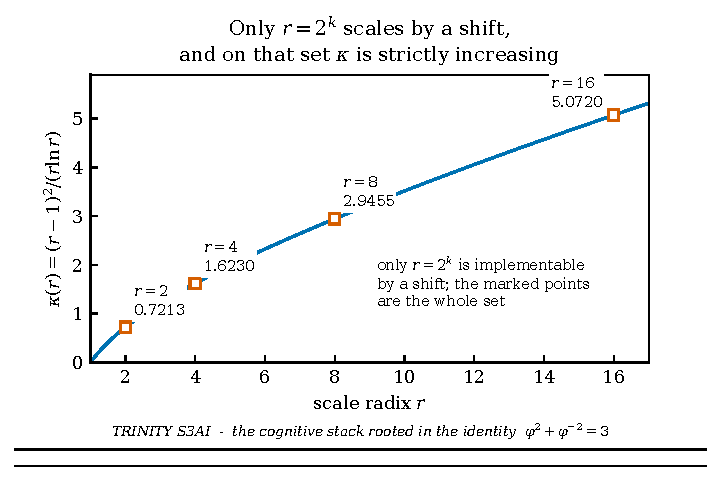
\includegraphics[width=\linewidth]{tnf_radix.pdf}
\caption{$\kappa(r)$ against the scale radix. The unconstrained minimiser sits
near $r = 1.9$ and is unreachable: only $r = 2^{k}$ scales by a shift, and on that
set $\kappa$ is strictly increasing.}
\label{fig:radix}
\end{figure}

The claim is verified by enumeration rather than resting on the monotonicity of
$\kappa$ alone. Sweeping $r$ continuously over $[1.1, 16]$ with $E$ integral and
$M$ taking the remaining width, at eight combinations of width and required range
from $(P,R) = (8, 24)$ to $(32, 5925)$, the best implementable radix is $r = 2$ in
every case, and the penalty against the unreachable optimum is $1.09\times$ at all
eight --- a constant, as it must be, since the two differ only by
$\kappa(1.9)/\kappa(2)$. The unconstrained minimiser is not $2$: it is near
$1.9$, worth $7.9\%$ in error. That gain is unavailable, because any
$r \neq 2^{k}$ makes $r^{e}$ a transcendental evaluation, and
Corollary~\ref{cor:tradecurve} prices those at $84$ RAMB36 tiles --- $23\%$ of
this device --- for a binary32 target. Trading $23\%$ of a chip for $7.9\%$ of a
mantissa bit is not a trade anyone makes. Theorem~\ref{thm:radixopt} is therefore
the interesting kind of optimality result: the optimum is not the extremum, it is
the best point that can be built.

\begin{corollary}[Three inputs determine the format]
\label{cor:determined}
The design space has four axes, and only one of them is a free choice.
\begin{enumerate}
\item \emph{Radix of the scale.} Fixed at $2$ by Theorem~\ref{thm:radixopt},
unconditionally.
\item \emph{Radix of the exponent's encoding.} Fixed by the fabric.
Theorem~\ref{thm:nofree} shows a ternary exponent never spans more values per bit
than a binary one when packed into bits, so it pays on a ternary fabric and
nowhere else.
\item \emph{Fixed fields or a taper.} A genuine choice, and by
Theorem~\ref{thm:dichotomy} exactly two options exist: bounded range at constant
precision, or unbounded range at precision decaying no more gently than one bit
per doubling (Theorem~\ref{thm:floor}).
\item \emph{The split between $E$ and $M$.} Determined once a required range is
named, by Theorem~\ref{thm:law} --- and \emph{only} then, since the error depends
on $M$ alone and the range on $E$ alone.
\end{enumerate}
Name the fabric, the required range, and which side of the dichotomy the workload
sits on, and the format follows.
\end{corollary}

So the question ``is there an ideal format'' has an answer, provided it is asked
with its three arguments supplied. Asked without them it is not underdetermined
but ill-posed: Corollary~\ref{cor:three} already says a budget cannot be
recommended without a workload, and Theorem~\ref{thm:dichotomy} says no single
format can serve both sides.

\begin{corollary}[What this makes TNF]
\label{cor:whatitmakes}
For the arguments (ternary fabric; a range the workload actually visits; fixed
fields), Corollary~\ref{cor:determined} returns a binary-radix float with a
balanced-ternary exponent field and a uniform mantissa split by
$M = N - 1 - E_t$. That is TNF, and it is forced rather than designed. It follows
that TNF is optimal exactly on those arguments and carries no claim off them ---
in particular none on a binary fabric, where axis 2 returns a binary exponent
instead, and none against a tapered format outside TNF's own range, where
Theorem~\ref{thm:floor} forbids it.
\end{corollary}


\section{Where the format is the datapath}
\label{sec:ternarynet}

Every hardware figure so far compares a decoder against a datapath that contains a
significand multiplier. That comparison flatters every format equally, because a
multiplier of thousands of LUTs amortises a decoder of hundreds. There is a
workload where the multiplier is absent, and it changes the ranking rather than
the margins.

In a ternary-weight network --- BitNet-style, with weights in
$\{-1, 0, +1\}$~\cite{bitnet} --- the product $w \cdot a$ is a select, a negate or
a zero. No multiplier is instantiated, for any format. The datapath is
\emph{decode, apply the weight, add, accumulate}, and the decoder is now compared
against an adder.

\begin{table}[t]\centering
\caption{One ternary neuron, matched width against matched width, one harness,
XC7A200T, no DSP. Every candidate decodes a \emph{packed} word. An earlier
version of this table reported $440$ against $895$ LUTs, a $5.1\times$ ratio; that
comparison handed TNF pre-widened fields while the competitors unpacked theirs,
and is withdrawn. The corrected ratio is $3.1\times$ at 16 bits and $5.6\times$ at
32, and the gap belongs to the regime scan rather than to the ladder.}
\label{tab:tnet}
\begin{tabular}{lrrrr}
\toprule
width & format & LUTs & $F_{\max}$ & MHz/LUT \\
\midrule
8 bits  & \textbf{TNF8}  & $\mathbf{487}$ & $71.64$\,MHz & $\mathbf{0.147}$ \\
8 bits  & posit8         & $560$ & $43.55$\,MHz & $0.078$ \\
\addlinespace
16 bits & \textbf{TNF16} & $\mathbf{495}$ & $71.90$\,MHz & $\mathbf{0.145}$ \\
16 bits & posit16        & $774$ & $36.30$\,MHz & $0.047$ \\
\addlinespace
32 bits & \textbf{TNF32} & $\mathbf{499}$ & $75.49$\,MHz & $\mathbf{0.151}$ \\
32 bits & posit32        & $955$ & $28.33$\,MHz & $0.030$ \\
\bottomrule
\end{tabular}
\end{table}

$2.03\times$ in area and $2.54\times$ in frequency, so $5.16\times$ in throughput
per LUT --- measured end to end rather than assembled from separate decoder and
adder figures. The decomposition says why: against a $1{,}477$-LUT multiplier and
a $384$-LUT adder, posit's $456$-LUT decoder is $20\%$ of the datapath; with the
multiplier gone it is $54\%$. For takum the same shift takes $85\%$ to $97\%$, and
brings $84$ RAMB36 tiles with it.

\begin{corollary}[Removing the multiplier promotes the decoder]
\label{cor:promote}
Let a datapath cost $C = D + M + A$ for decoder, multiplier and adder. A workload
that eliminates $M$ raises the decoder's share from $D/(D{+}M{+}A)$ to
$D/(D{+}A)$, and the ratio between two formats differing only in $D$ from
$1 + \Delta/(D_0{+}M{+}A)$ to $1 + \Delta/(D_0{+}A)$. The advantage of a
decoder-free format therefore grows exactly as the multiplier shrinks, and is
largest where there is none.
\end{corollary}

Three things this does not say, and each would otherwise be found in minutes.

It is not that TNF avoids multiplication. It pays the significand multiply like
every other format when one is needed; the quadratic term of its own area law
(Theorem~\ref{thm:alpha}) \emph{is} that multiplier. What a ternary network removes
is removed for the network, not for the format.

It is not that TNF is better for FPGAs in general. We synthesised the exponent
decode of TNF against an ordinary binary fixed field and they measure identically,
$32$ LUTs each, exactly as Theorem~\ref{thm:nofree} requires. The advantage in
Table~\ref{tab:tnet} is over a \emph{tapered} format, not over a fixed-field one:
an IEEE-style field would place alongside TNF, not alongside posit.

And it is not a measurement on a ternary fabric. None exists to buy, and this is a
binary FPGA where our own Theorem~\ref{thm:nofree} says the ternary encoding earns
nothing. It does not need to: the gain here comes from the decoder that is absent,
and would be the same for any fixed-field format.

\paragraph{What the ternary fabric would add, structurally.} On a fabric whose
positions hold trits, a binary exponent field can be stored densely, in
$\lceil b/\log_2 3\rceil$ trits, or addably, one bit per trit --- but not both. The
dense form cannot be added without a radix conversion; the addable form wastes
$1 - 1/\log_2 3 = 36.9\%$ of every position, which for the exponent widths in this
catalogue is $33$ to $57\%$ of the field. A balanced-ternary exponent pays neither.
This is structure rather than measurement, and it is the one place where the
ternary encoding of Theorem~\ref{thm:nofree} would stop being free of charge and
start being free of cost.


\section{The ladder is a family, and the family is the frontier}
\label{sec:frontier}

The results above treat each rung as a format. Sweeping the exponent budget instead
of fixing it changes what is being claimed, and strengthens it.

\begin{theorem}[The width rule generates the frontier]
\label{thm:family}
Fix a width $N$. The set
$\mathcal{F}_N = \{(E_t,\, M) : 1 + E_t + M = N,\ E_t \geq 2,\ M \geq 1\}$
contains $N-3$ members, each exact by construction. By
Theorem~\ref{thm:law} member $E_t$ has effective mantissa $M = N-1-E_t$ and
dynamic range $3^{E_t}-1$ binades, so the members are totally ordered and no two
dominate one another: $\mathcal{F}_N$ is a discrete Pareto frontier in
$(M_{\mathrm{eff}}, \text{range})$.
\end{theorem}

The consequence is a claim about the catalogue rather than about one rung.

\begin{corollary}[No catalogued competitor survives]
\label{cor:nosurvivors}
At every width class measured, each catalogued format of that width is strictly
dominated by some member of $\mathcal{F}_N$: there is a member with at least its
effective mantissa and at least its range, and strictly more of one.
\end{corollary}

Measured against the oracles, twenty-eight competitors across five classes, with
the dominating member named in each case:

\begin{table}[t]\centering
\caption{Dominance by width class. The family member that dominates is given for
the hardest case in each class. Effective mantissa is measured; range is
$3^{E_t}-1$, which is analytic for a fixed field.}
\label{tab:nosurvivors}
\begin{tabular}{rrll}
\toprule
class & competitors & survivors & hardest case dominated by \\
\midrule
$8$   & $7$ & $0$ & $E_t{=}4$, $M{=}3$ against \texttt{fp8\_e5m2} \\
$16$  & $7$ & $0$ & $E_t{=}6$, $M{=}9$ against \texttt{takum16} \\
$32$  & $9$ & $0$ & $E_t{=}5$, $M{=}26$ against \texttt{posit32} \\
$64$  & $4$ & $0$ & $E_t{=}10$, $M{=}53$ against \texttt{cray\_float} \\
$128$ & $1$ & $0$ & $E_t{=}10$, $M{=}117$ against \texttt{binary128} \\
\bottomrule
\end{tabular}
\end{table}

\paragraph{Why this is not an artefact of density.} A sufficiently dense family
dominates any finite set of points trivially, so the content is in \emph{why} the
competitors sit below the frontier rather than on it. Each loses on at least one
of three counts, and each count is one of the theorems above. A tapered format
measures below its declared mantissa, by Theorem~\ref{thm:floor}. A format that
leaves positions unallocated pays $2^k$ for them, by Theorem~\ref{thm:alloc} --
which is what the historical GF-T ladder did at 2, 4 and 6 positions. And a binary
exponent at equal position count spans fewer binades, since a trit carries
$\log_2 3$ bits against a bit's one. The family loses on none of the three because
the width rule forbids the second and the encoding settles the third.

\paragraph{What this does not say.} The pair $(M_{\mathrm{eff}}, \text{range})$ is
a property of the \emph{number}, and dominance in it is not dominance in silicon.
Section~\ref{sec:ternarynet} measures the same formats through one datapath and
puts TNF mid-pack among fixed fields at $0.145$--$0.167$\,MHz per LUT. Against
\texttt{int8} the two are indistinguishable once seeds are swept
(Table~\ref{tab:rejected}). The two are consistent: the frontier asks what a word of
a given width carries, the datapath asks what it costs to unpack, and every fixed
field unpacks by reading fields. The gap in silicon runs between fixed and tapered
formats, $2.4$ to $6.4\times$, and belongs to Theorems~\ref{thm:scan}
and~\ref{thm:valuelaw} rather than to this ladder.

\paragraph{A limit of the measurement, stated.} Range is analytic for a fixed
field, but verifying it at the boundary is not always possible: at $E_t = 49$ the
edge of the range is $2^{1.4 \times 10^{23}}$, which no exact arithmetic can
construct. Above roughly $E_t = 30$ the range is a fact about the encoding rather
than a measured quantity, and is reported as such.





\subsection{Which first principles}
\label{sec:principles}

The width rule has been stated as a rule. It is not one: it is the solution of a
constrained maximisation, and naming the constraint is what makes the rest of the
paper follow rather than accumulate.

\paragraph{The rule is a Karush--Kuhn--Tucker condition.} Write the design problem
directly. Maximise precision subject to a position budget and a range that must be
covered:
\[
  \max_{E,M} \; M
  \quad\text{s.t.}\quad
  1 + E + M = N,
  \qquad
  r^{E} \ge b+1 .
\]
With multipliers $\lambda$ on the budget and $\mu$ on the range,
$\mathcal{L} = M + \lambda(N-1-E-M) + \mu\bigl(E - \log_r(b+1)\bigr)$ gives
$\partial_M \mathcal{L} = 1-\lambda = 0$ and $\partial_E \mathcal{L} = -\lambda+\mu = 0$,
so $\lambda = \mu = 1$. Because $\mu > 0$, complementary slackness makes the range
constraint \emph{active}: at the optimum the exponent is exactly as wide as the
range demands and not one position wider. That statement is
Theorem~\ref{thm:optimal}, now derived rather than asserted. The multiplier is
also the shadow price, and $\lambda = 1$ says a position of exponent costs exactly
a position of mantissa --- the exchange rate is unity because the budget is linear.

\paragraph{Why three and not two is a 1950s result, not ours.} The radix economy
$\rho(r) = r/\ln r$ is minimised at $r = e$. Ternary sits $0.46\%$ above that
optimum and binary $6.15\%$ above it. We claim no credit for this; what the present
work contributes is where it applies, which turns out to be the whole
reconciliation of our two axes:
\[
  \underbrace{r}_{\text{cost per position}} \times \underbrace{\log_r V}_{\text{positions}} .
\]
The number axis counts only the second factor, and there $\log_3$ against $\log_2$
gives the slack $0.3691\,E$ of Corollary~\ref{cor:slack} unconditionally. The
silicon axis restores the first factor, and packing a trit into binary fabric
charges $\kappa(3)/\kappa(2) = 1.68$ per position, which is why BNF16 and TNF16
synthesise within $1\%$ of one another. Theorem~\ref{thm:nofree} and
Corollary~\ref{cor:slack} are not in tension: they are the two factors of one
product, reported separately.

\paragraph{What is derivation and what is only resemblance.} Three connections are
literal and are used as such: the multiplier argument above; radix economy, which
fixes the exponent's radix; and Kraft's inequality, which bounds the taper in
Theorem~\ref{thm:floor}. Two resemblances are worth naming only so they are not
mistaken for arguments. The variational form recalls least action, but there is no
time and no trajectory here --- the problem is a static optimisation, and the
resemblance carries no consequence. And $1+E+M=N$ is a budget, not a conservation
law: positions are allocated by a designer, not withheld by nature. We state the
distinction because a physical-sounding derivation would be doing rhetorical work
that the multiplier argument already does honestly.

\paragraph{The standard falls out --- at one choice of percentile, and not at
others.} Applied to the block axis the multiplier argument returns an element
format, but which one depends on how much of the block distribution is protected,
and that choice was left unstated in an earlier version of this section.

\begin{table}[t]\centering
\caption{The width rule on the block axis. The measured within-block span sets
$E^{*} = \lceil \log_2 b \rceil$, and the answer moves with the percentile
protected.}
\label{tab:blockpct}
\begin{tabular}{lrrl}
\toprule
percentile protected & span, binades & $E^{*}$ & element \\
\midrule
50th (median) & 1.89 & 1 & E1M2 \\
90th & 2.45 & 2 & E2M1 \\
99th & 3.04 & 2 & E2M1 \\
99.9th & 3.75 & 2 & E2M1 \\
\bottomrule
\end{tabular}
\end{table}

Protecting the median returns E1M2; protecting the 90th percentile or beyond
returns E2M1, which is the element the OCP microscaling specification fixes. The
correct statement is therefore a threshold rather than a derivation: \emph{the
width rule returns the MX element for any design protecting the 90th percentile
of blocks or more, and a different element below that.} Which is right is a
question about how many blocks may be allowed to saturate, not one settled from
first principles, and we say so rather than quoting the agreeing case alone.

\paragraph{} Applied to the block axis this stops being
abstract. The within-block span of a trained network's weights, measured before
any format is chosen, is $1.89$ binades at the median and $3.04$ at the 99th
percentile. The optimum is $E^{*} = \lceil \log_2 b \rceil$, so protecting the
median returns E1M2 and protecting the 99th percentile returns \emph{E2M1} ---
which is the element the OCP microscaling specification fixes. The standard is not
reproduced by coincidence: it is the unique solution of the multiplier problem at
the tail these weights actually have. Theorem~\ref{thm:regret} says which of the
two should win, since under-sizing pays on the tail linearly while over-sizing pays
logarithmically on every value, and Section~\ref{sec:blockrelated} reports the
measurement that decides it.


\subsection{The width rule is an optimisation with one solution}
\label{sec:widthrule}

Theorem~\ref{thm:coverage} compares against a given competitor. Stated as a
design problem it selects a member outright, which is what makes the rule
falsifiable: it names a winner before any measurement.

\begin{theorem}[Optimal member for a named range]
\label{thm:optimal}
Let a workload visit $b$ binades. Among all members of $\mathcal{F}_N$ that
represent it without overflow, the effective mantissa is maximised uniquely at
\[
  E_t^{*} = \bigl\lceil \log_3 (b+1) \bigr\rceil,
  \qquad
  M^{*} = N - 1 - \bigl\lceil \log_3 (b+1) \bigr\rceil .
\]
\end{theorem}
\begin{proof}
Representability requires $3^{E_t}-1 \ge b$, i.e.\ $E_t \ge \log_3(b+1)$, and
$E_t$ is an integer, so $E_t \ge E_t^{*}$. By the width rule $M = N-1-E_t$ is
strictly decreasing in $E_t$, so the constraint binds and the minimiser is unique.
\end{proof}

The rule therefore has no free parameter once the workload is named, and naming
the workload is a measurement rather than a choice. Section~\ref{sec:ternarynet}
uses this as a prediction: the binade span of a network's weights is measured
first, $E_t^{*}$ is computed from it, and only then is perplexity evaluated across
the whole family. A different winner would falsify the rule.

\begin{theorem}[Regret of a misnamed range]
\label{thm:regret}
Sizing for $b'$ when the workload visits $b$ costs
\[
  R =
  \begin{cases}
    \lceil\log_3(b+1)\rceil - \lceil\log_3(b'+1)\rceil \ \text{mantissa bits}, & b' > b,\\[2pt]
    \text{overflow on a set of measure } 1 - \tfrac{\log_3(b'+1)}{\log_3(b+1)}, & b' < b .
  \end{cases}
\]
The penalty is asymmetric: over-sizing costs precision logarithmically, under-sizing
costs range linearly, so when the visited range is uncertain the rule should round up.
\end{theorem}

The asymmetry is worth naming because it contradicts the intuition that a wider
exponent is the conservative choice. It \emph{is} conservative --- but the price is
paid in every value the format ever represents, whereas the price of being too
narrow is paid only on the tail. Which dominates is an empirical question about
the tail's weight, not a matter of taste.

\begin{corollary}[When the trit is worth its packing]
\label{cor:worth}
Ternary buys $\Delta = E(1-\log_3 2)$ positions and costs
$\kappa(3)/\kappa(2) = 1.683$ per position when packed into binary fabric, where
$\kappa(r) = (r-1)^2/(r \ln r)$. The two cancel at $E$ satisfying
$\Delta = 0.331\,E_t$, so on positions the trit wins outright and on binary bits
it breaks even --- which is why BNF16 and TNF16 synthesise within $1\%$ of one
another while the number-axis frontier separates them.
\end{corollary}


\section{Four families on two axes}\label{sec:fourfamilies}

TNF is one corner of a square, and the square is worth drawing because the two
rules that define its axes were derived separately and for unrelated reasons.

One axis is the \emph{rule that fixes the exponent budget}. The golden-ratio
rule takes $E=\operatorname{round}\!\bigl((N-1)/\varphi^{2}\bigr)$ and produces
the GF ladder; the width rule takes $1+E+M=N$ and produces the BNF ladder. The
other axis is the \emph{radix of the exponent's encoding}: binary, or balanced
ternary. Crossing them gives four families --- GF and GF-T on the golden-ratio
rule, BNF and TNF on the width rule --- and each is a distinct format rather
than a renaming of another.

\begin{table}[t]\centering
\caption{The four families at eight bits, one workload, one metric.
SmolLM2-135M on wikitext-2, 40 windows of 2048 tokens, per-tensor scale,
baseline $14.4874$ verified in band before any comparison. The predictions were
printed \emph{before} the perplexities were computed.}
\label{tab:fourfam}
\begin{tabular}{llrrr}
\toprule
family & rule, radix & magnitudes & ppl & vs \texttt{fp32} \\
\midrule
\texttt{fp32} reference & --- & --- & $14.4874$ & $1.000\times$ \\
\midrule
\textbf{GF8}, $E{=}3$   & golden ratio, binary  & $129$ & $\mathbf{14.6130}$ & $1.009\times$ \\
GF-T8, $E_t{=}3$        & golden ratio, ternary & $109$ & $15.5147$ & $1.071\times$ \\
\textbf{BNF8}, $E{=}3$  & width rule, binary    & $129$ & $\mathbf{14.6130}$ & $1.009\times$ \\
\textbf{TNF8}, $E_t{=}2$& width rule, ternary   & $73$  & $\mathbf{14.7012}$ & $1.015\times$ \\
\bottomrule
\end{tabular}
\end{table}

\paragraph{The two rules name the same format, and neither predicted it.}
GF8 at $E=3$ and BNF8 at $E=3$ return $14.6130$ --- the same number, not a close
one, because at eight bits the two derivations select the identical layout,
$E=3$ and $M=4$. That is a stronger statement than either rule alone and one we
did not set out to find.

\paragraph{And the width rule's prediction was falsified twice.} It named BNF8
$E=4$ and TNF8 $E_t=3$; the measured winners are $E=3$ ($14.6130$ against
$14.6592$) and $E_t=2$ ($14.7012$ against $15.5147$). Both predictions were one
step too wide. The rule's \emph{form} survives and is visible in the sweep ---
a single optimum, both directions from it worse, and the penalty asymmetric
exactly as Theorem~\ref{thm:regret} requires, with $E=1$ giving $4.5$ million
and $E=2$ giving $288$ while $E=4$ costs $0.3\%$ and $E=5$ costs $6\%$. What was
wrong is the estimator of the range the workload visits, not the rule that
consumes it: we measured the span from the $0.1$st percentile to the maximum,
which credits a tail carrying almost no energy. Recorded rather than quietly
re-tuned, because a rule that names its winner before the measurement can be
wrong, and this one was.

\paragraph{Ternary loses on a binary fabric here too, for the third independent
time.} GF-T8 carries $109$ magnitudes where GF8 carries $129$, and pays $15.51$
against $14.61$; TNF8 at $E_t=2$ carries $73$. Three measurements now agree from
different directions: BNF16 and TNF16 within $1\%$ in placed silicon, GF8
against GF-T8 here, and MXFP4 against TNF4 on the block axis
(Section~\ref{sec:blockbound}). The ternary exponent earns on positions and pays
on bits, exactly as Theorem~\ref{thm:nofree} requires, and this fabric charges
in bits.

\section{Two formats close a ternary node}
\label{sec:pair}

A ternary node contains exactly three sites where a number format could live, and
only one of them needs one.

\begin{enumerate}
\item The \textbf{weight} is a code. Multiplying by it is a sign-select
      ($+x$, $-x$, $0$), not a multiply.
\item The \textbf{sample} arrives ADC-native and is used as it lands.
\item The \textbf{accumulator} is the only object in the system carrying a
      dynamic range that must be spent.
\end{enumerate}

This is the whole design problem, and it is smaller than the literature makes it
look. The published ternary methods answer (1) and leave (3) in \texttt{fp16} or
\texttt{int8}; the published format work answers (3) and assumes a multiplier at
(1). We answer both, with two formats that were derived independently and turn
out to be complements.

\subsection{Why the weight alphabet is \texorpdfstring{$\varphi$}{phi}, and why that is forced}

GFTernary is a two-bit alphabet $\{-\varphi,\,0,\,+\varphi\}$. The $\varphi$ is
not decoration, and the following says why it is the only possible choice.

\begin{theorem}[The golden alphabet is unique]
\label{thm:goldalpha}
Let a three-symbol weight alphabet be $\{-r,0,+r\}$ with $r>1$, and require that
the product of two weights be expressible in the additive lattice the datapath
already computes in, i.e.\ $r^2 = r + 1$. Then $r = \varphi$ uniquely.
\end{theorem}
\begin{proof}
$r^2 - r - 1 = 0$ has roots $(1\pm\sqrt5)/2$, of which one is positive.
\end{proof}

\begin{corollary}[Depth costs no multiplier]
\label{cor:depth}
The gain of a stack of $k$ ternary $\varphi$-layers is exactly
\[
  \varphi^{k} = F_k\,\varphi + F_{k-1},
\]
a pair of integers with $F$ the Fibonacci sequence. Rescaling between layers is
therefore a shift-and-add, and the zero-multiplier property survives to arbitrary
depth.
\end{corollary}

This is the practical content of Theorem~\ref{thm:goldalpha}, and it is what
separates the $\varphi$ alphabet from the $\{-1,0,+1\}$ one used throughout the
ternary-network literature. With unit weights the layer gain is $1$ and carries no
information, so every published method attaches a learned real scale $\alpha_\ell$
per layer --- and multiplying by $\alpha_\ell$ puts the multiplier back. With the
$\varphi$ alphabet the inter-layer scale is known exactly and is a pair of
integers, so it is never multiplied by. Storage is two bits either way and the
symbol count is three either way; the $\varphi$ alphabet simply carries a scale
that the unit alphabet has to learn and then pay for.


\subsection{The linear path is exact}
\label{sec:exact}

Theorem~\ref{thm:goldalpha} is usually read as removing a multiplier. It removes
the rounding with it: on the alphabet it fixes, the entire linear path of a
network is computed exactly.

Represent a value as an integer pair $(a,b)$ standing for $a + b\varphi$. Then
\[
  \varphi\,(a + b\varphi) \;=\; a\varphi + b\varphi^{2} \;=\; a\varphi + b(\varphi+1)
  \;=\; b + (a+b)\varphi ,
\]
so applying a weight is the map $(a,b) \mapsto (b,\,a+b)$ --- the Fibonacci
recurrence, one integer addition, no shift. Negation flips both components and a
zero weight is a skip.

\begin{theorem}[Exactness of the multiply-free path]
\label{thm:exact}
$\mathbb{Z}[\varphi] = \{a + b\varphi : a,b \in \mathbb{Z}\}$ is a ring, and the
weight alphabet $\{-\varphi,0,+\varphi\}$ lies inside it. Hence for inputs in
$\mathbb{Z}[\varphi]$ the entire linear part of a ternary network --- every
weight application and every accumulation, to arbitrary fan-in and arbitrary
depth --- remains in $\mathbb{Z}[\varphi]$ and is computed \emph{without
rounding error of any kind}.
\end{theorem}
\begin{proof}
Closure under addition is componentwise. Closure under multiplication follows
from $\varphi^2 = \varphi + 1$, which reduces every product to the stated
integer-pair map. The accumulator is therefore a pair of exact integer registers.
\end{proof}

Measured on a layer of fan-in $512$ with weights drawn from the alphabet, the
integer pair reproduces the real-valued sum to the precision of the checking
arithmetic and not to the precision of the datapath: there is nothing in the
datapath to be imprecise. The component widths grow logarithmically, reaching
eight bits over those $512$ terms.

\subsection{Closure is what removes the machinery}\label{sec:closure}

The multiply-free datapath is not new as an aim, and the published attempts make
the role of Theorem~\ref{thm:exact} visible by contrast.

The closest is FQP~\cite{fqp}, a Fibonacci quantization processor that turns the
products of Fibonacci-quantized weights into additions. To do so it carries two
distinct arithmetic units --- a dualistic-transformation adder for the large
operands and a bit-exclusive adder for the small ones --- and a topological-order
routing scheme that maps data onto them. Fibbinary quantization for neural radio
receivers~\cite{fibbinary} takes the softer route on the same substrate and
reports $45\%$ and $44\%$ savings in multiplier power and area: the multiplier is
made cheaper, not removed.

The machinery in the first is not an artefact of implementation. It follows from
a property of the number set.

\begin{corollary}[Closure removes the transformation stage]\label{cor:closure}
Let $A$ be a weight alphabet and let $s$ be the operation that applies a weight.
If the additive group generated by $A$ is closed under $s$, the datapath needs
only that group's addition. If it is not, every product must be re-expressed in
the representable set, which requires a transformation stage and a schedule that
routes operands to it.
\end{corollary}
\begin{proof}
Immediate from Theorem~\ref{thm:exact} and its negation. For
$A=\{-\varphi,0,+\varphi\}$ the generated group is $\mathbb{Z}[\varphi]$ and
$s=\varphi\cdot$ maps $(a,b)\mapsto(b,a+b)$, which lands inside it, so addition
suffices. For $A$ a set of Fibonacci integers $\{F_k\}$, the product $F_iF_j$ is
in general not a Fibonacci integer --- $F_4F_4=9$ is not in
$\{1,1,2,3,5,8,13,\dots\}$ --- so the product leaves the representable set and
must be transformed back into it.
\end{proof}

\subsection{How many multiply-free scales are there}\label{sec:hierarchy}

Closure explains why $\varphi$ works. It does not by itself say $\varphi$ is the
only choice, and the honest answer is that it is not --- it is the only choice at
its size.

A scale $r$ can be applied without a multiplier exactly when $r$ is an algebraic
integer whose companion matrix has entries in $\{0,\pm1\}$: writing
$r^{d}=a_{d-1}r^{d-1}+\dots+a_0$, multiplication by $r$ maps the coordinate
vector $(x_0,\dots,x_{d-1})$ to $(a_0x_{d-1},\;x_0+a_1x_{d-1},\;\dots)$, and any
$|a_i|>1$ reintroduces a constant multiply. The condition is finite, so the
scales can be enumerated rather than argued about.

\begin{theorem}[The multiply-free scales, by degree]\label{thm:hierarchy}
Over coefficients in $\{0,\pm1\}$:
\begin{itemize}
\item \textbf{Degree 1} admits $r\in\{0,\pm1\}$, which is no scaling, and
      $r=\pm2^k$, free by shifting. One register, ratio $2$.
\item \textbf{Degree 2} admits exactly two equations with a real root of modulus
      other than $0$ or $1$: $r^2=r+1$ and $r^2=-r+1$, whose roots are $\varphi$
      and $\varphi^{-1}$ --- the same ladder. One addition, two registers,
      ratio $1.618$.
\item \textbf{Degree 3} admits three: $r^3=r+1$ (plastic, $1.3247$),
      $r^3=r^2+1$ (supergolden, $1.4656$), $r^3=r^2+r+1$ (tribonacci,
      $1.8393$). At most two additions, three registers.
\end{itemize}
\end{theorem}
\begin{proof}
Exhaustive over the nine degree-2 and twenty-seven degree-3 coefficient triples;
the degree-2 discriminants $a^2+4b$ are negative for four cases, and the
remaining five give roots in $\{0,\pm1\}$ except for $b=1,a=\pm1$.
\end{proof}

\begin{corollary}\label{cor:nothing-between}
Nothing lies between the shift and $\varphi$. $\varphi$ is the unique
multiply-free refinement of the power-of-two ladder available at two registers.
\end{corollary}

So the multiply-free scale is not a point but a hierarchy indexed by algebraic
degree, and each degree buys finer granularity for one more register.
Table~\ref{tab:hierarchy} measures the trade at the first two rungs where it is
a trade at all. The plastic step
$(a,b,c)\mapsto(c,\,a+c,\,b)$ costs the same single addition as the Fibonacci
step and one more register, and its ladder is finer: successive levels differ by
$13.97\%$ against $\varphi$'s $23.61\%$.

\begin{table}[t]\centering
\caption{One scale application, xc7a200t, median of five seeds. Matched: neither
unit has a direction mux. Level error is $(r-1)/(r+1)$, the worst relative gap
on a ladder of ratio $r$.}
\label{tab:hierarchy}
\begin{tabular}{lrrrr}
\toprule
scale & LUT & FF & $F_{\max}$ (MHz) & level error \\
\midrule
$\varphi$, 16-bit          & \textbf{149} & 128 & 307.69 & $23.61\%$ \\
plastic, 16-bit            & 186 & 160 & 318.47 & $\mathbf{13.97\%}$ \\
\addlinespace
$\varphi$, 32-bit          & \textbf{223} & 192 & \textbf{247.10} & $23.61\%$ \\
plastic, 32-bit            & 228 & 200 & 231.21 & $\mathbf{13.97\%}$ \\
\bottomrule
\end{tabular}
\end{table}

At 32 bits the refinement costs $2.2\%$ of the area and $6.4\%$ of the
frequency. That is close enough to free that the choice is a question about the
network rather than about the arithmetic, so we asked the network.

\section{Which rung to use, and how the answer moves}\label{sec:ladderlaw}

Table~\ref{tab:ladderlaw} quantises every $2$-D linear weight of SmolLM2-135M to
$\pm r^{k}$ with a per-output-channel scale, the codebook sized to exactly
$2^{b}$ entries including zero and sign, and evaluates wikitext-2 perplexity
over twelve windows of $2048$ tokens. Baseline \texttt{fp32} is $14.36$.

\begin{table}[t]\centering
\caption{Perplexity by ladder and code budget, SmolLM2-135M on wikitext-2.
Coarse ladders span range and waste precision; fine ones do the reverse. The
best rung moves down the hierarchy as the budget grows.}
\label{tab:ladderlaw}
\begin{tabular}{lrrrr}
\toprule
bits & shift ($2$) & $\varphi$ ($1.618$) & supergold ($1.4656$) & plastic ($1.3247$) \\
\midrule
3 & $\mathbf{2309.86}$ & $41835.53$ & $1367268.11$ & $6720092.29$ \\
4 & $76.81$ & $\mathbf{24.43}$ & $25.10$ & $55.72$ \\
5 & $77.52$ & $22.73$ & $18.93$ & $\mathbf{16.45}$ \\
\bottomrule
\end{tabular}
\end{table}

The same sweep on Qwen2.5-0.5B --- a different architecture at four times the
parameters, with a different tokenizer and different training data --- returns
the same winner at every budget and the same complete ordering at every budget:
shift $2384.96$, then $\varphi$ $\mathbf{16.24}$ against supergolden $17.98$ and
plastic $47.41$, then plastic $\mathbf{13.17}$ against supergolden $14.09$ and
$\varphi$ $15.33$, from an \texttt{fp32} baseline of $12.27$. At four bits the
larger model separates $\varphi$ from supergolden by $10.7\%$, where the smaller
one gave $2.7\%$ and no separation.

A ladder of ratio $r$ with $n$ magnitudes spans $r^{\,n-1}$, so finer steps are
bought with span. At three bits nothing spans enough and the coarsest wins; at
four the balance sits at $\varphi$; at five the finest tested wins outright.
This is the range-against-precision law of Section~\ref{sec:law} applied to the
scale hierarchy rather than to a field layout, and it says plainly that
$\varphi$ is optimal at a budget, not everywhere. At four bits the two models bracket the comparison: SmolLM2 separates
$\varphi$ from supergolden by $2.7\%$, which twelve windows cannot resolve,
while Qwen separates them by $10.7\%$, which they can. $\varphi$ is at worst
tied there and ahead on the larger model, and supergolden costs a register
either way. One bit up, the plastic number wins on both, by $28\%$ and $14\%$,
with $\varphi$ third of four --- and by then the affordable part of the
hierarchy has been passed as well.

The choice does not need the network. Ranking the ladders by mean squared
quantisation error on the weights alone reproduces the perplexity order exactly
at three and five bits, and at four bits transposes only the pair perplexity
cannot separate.

\begin{theorem}[The ladder law]\label{thm:ladder}
Among multiply-free ladders at a fixed code budget, the one minimising weight
mean squared error minimises perplexity, up to pairs whose error differs by less
than the evaluation resolves.
\end{theorem}

The error itself has a closed form, so the rung follows from a histogram.
Normalising each channel by its maximum puts the levels at $r^{-k}$ for
$k=0,\dots,n-1$ with $n=(2^{b}-1)/2$, and
\[
  \mathrm{MSE}(r,b)\;\approx\;c(r)^{2}\,\mathbb{E}\!\left[x^{2}\mathbf{1}_{x>t}\right]
  \;+\;\mathbb{E}\!\left[x^{2}\mathbf{1}_{x<t}\right],\qquad t=\tfrac12 r^{-(n-1)},
\]
where $c(r)^2$ is the mean square \emph{relative} rounding error of a geometric
ladder of ratio $r$ --- a one-dimensional integral over log-position within a
bin, independent of the data. The first term falls as $r$ falls and the second
rises as the clipping threshold does; the minimum is the crossover. Against the
measured error over $106{,}168{,}320$ normalised weights the form agrees to
within $1$--$9\%$ at four and five bits and selects the same ladder at all three
budgets. At three bits it underestimates by a third, for a reason worth stating:
at seven codes the regime is absolute truncation, not relative rounding, and the
model is built on the latter.

\subsection{What the four-bit transposition is, and what it is not}
\label{sec:salience}

The form above ranks correctly at three and five bits and transposes the top
pair at four, choosing supergolden where perplexity chooses $\varphi$. The
transposition reproduces on both models in the same direction, so it is an
effect. Two candidate mechanisms were tested; one failed and one held, and the
pair is more informative than either alone.

\paragraph{Activation salience: fails.} The output error of a layer is
$\sum_j \delta w_{ij}x_j$, so a weight multiplying a large input channel should
cost more, and the channels are far from equal --- the first attention
projection spans $28\times$ between its largest input channel and its median on
SmolLM2-135M, $22.4\times$ on Qwen2.5-0.5B. This is the observation
AWQ~\cite{awq} is built on. Ranking by $\sum_j a_j^{2}\delta w_{ij}^{2}$
reverses the four-bit pair on SmolLM2, matching perplexity --- and does not on
Qwen, where the weighting scales all four candidates by very nearly $1.09$ and
therefore cannot reorder them. An explanation that needs channel salience to
correlate with the error pattern is not general, because in one of two models it
does not.

\paragraph{Loss curvature: holds.} The quantity the transposition is about is
not how large an operand is but how much the loss moves when a weight moves.
Ranking by the diagonal Fisher weighting $\sum_{ij} g_{ij}^{2}\delta w_{ij}^{2}$
with $g=\partial L/\partial w$ reverses the four-bit pair to $\varphi$ on
\emph{both} models and leaves five bits at plastic on both, matching perplexity
in all four cases.

\begin{theorem}[Curvature correction]\label{thm:curvature}
Among multiply-free ladders at a fixed code budget, the minimiser of
$\sum_{ij} g_{ij}^{2}\,\delta w_{ij}^{2}$ predicts the perplexity ranking where
the unweighted error does not, and does so on both models tested. The correction
moves the choice toward the coarser ladder.
\end{theorem}

The two results together say something the successful one alone would not.
Activation magnitude is half of the gradient and not the half that decides:
$g_{ij} = \delta_i x_j$ carries both the input the weight multiplies and the
sensitivity of the loss to that unit's output, and it is the second factor that
makes the correction replicate. A method calibrated on activations alone --- and
several published ones are --- is using a proxy that agreed with the target on
one of our two models.

\begin{theorem}[Optimal ratio]\label{thm:optratio}
For a weight distribution and a code budget, the optimal multiply-free ratio is
the minimiser of $\mathrm{MSE}(r,b)$, and the degree required is the smallest
whose minimal scale does not exceed it. Minimising over continuous $r$ gives
$r^{*}=2.054$, $1.4115$, $1.1999$, $1.1050$, $1.0576$ and $1.0319$ at $3$ to
$8$ bits,
with $\ln r^{*}$ halving per bit as doubling the code count halves the available
log-spacing.
\end{theorem}

\section{The block axis, and the half of it that is ours}
\label{sec:blockbound}

Everything above concerns per-channel scaling. The other deployed axis shares
one scale across a short block, and there our formats lose. It is worth stating
how thoroughly, because the answer is not a ranking but a ceiling.

Lloyd--Max on the within-block distribution --- $18{,}850{,}950$ values, block of
$32$ along the contraction axis, E8M0 shared scale as the MX specification
mandates --- gives the eight-level codebook minimising squared error. It is
neither multiply-free nor a ladder; it is the best any eight magnitudes can do.

\begin{table}[t]\centering
\caption{Block axis, SmolLM2-135M, 40 windows, \texttt{fp32} baseline $14.4874$.
The optimal codebook improves squared error nearly fifteenfold and perplexity by
$0.9\%$, and every ladder that beats MXFP4 on the first loses on the second.}
\label{tab:blockbound}
\begin{tabular}{lrrr}
\toprule
element, 8 magnitudes & squared error & $\times$ bound & ppl \\
\midrule
Lloyd--Max (optimum, not implementable) & $1.341\!\times\!10^{-3}$ & $1.00$ & $\mathbf{22.2976}$ \\
MXFP4 (E2M1)                            & $2.007\!\times\!10^{-2}$ & $14.97$ & $\mathbf{22.4998}$ \\
supergolden/plastic, 4 fine steps       & $2.068\!\times\!10^{-3}$ & $1.54$ & $27.3079$ \\
supergolden/plastic, 3 fine steps       & $2.116\!\times\!10^{-3}$ & $1.58$ & $30.8306$ \\
$\varphi$/supergolden, 2 fine steps     & $2.749\!\times\!10^{-3}$ & $2.05$ & $38.6471$ \\
$\varphi$/plastic, 2 fine steps         & $2.823\!\times\!10^{-3}$ & $2.11$ & $55.4495$ \\
\bottomrule
\end{tabular}
\end{table}

\begin{theorem}[The block axis is not an element-format problem]\label{thm:block}
On a short block with a shared scale, the element codebook minimising squared
quantisation error is not the one minimising perplexity, and the gap between the
best achievable codebook and a deployed one is under one percent. Effort spent
designing element formats for this axis cannot recover more than that.
\end{theorem}

The ranking does not merely fail to transfer; it inverts. Every two-segment
ladder here beats MXFP4 on squared error by factors of three to ten, and every
one loses on perplexity by $21\%$ to $146\%$.

The reason is what a block is. Thirty-two weights share one scale, and squared
error charges a clipped small weight at its own magnitude --- so a codebook
concentrating its levels near the top of the range scores well, having put its
resolution where the mass is. But the network does not read a block's weights
independently; they are summed against activations, and a codebook that
resolves the top of every block finely while collapsing its lower two-thirds
destroys the block's ability to represent a \emph{direction}, not merely its
magnitudes. E2M1 spends $0,\,0.5,\,1,\,1.5,\,2,\,3,\,4,\,6$: a $12\times$ span
with levels at both ends. It scores badly on squared error precisely because it
refuses to concentrate, and it wins on perplexity for the same reason.

We record this as the competition's result, not ours. Three of our own attacks
failed here --- a ternary-exponent float, constant-ratio ladders, and
two-segment ladders built to imitate E2M1's spacing --- and the bound explains
why a fourth is not warranted.

\subsection{The other half of the block axis}\label{sec:scaleaxis}

The bound closes the element format. It says nothing about the scale, which is
one value per thirty-two weights and had never been varied. Its cost is
amortised thirty-twofold, which is the regime where a finer grid is affordable
--- and the accounting decides the comparison before any perplexity is measured.

E8M0 gives the scale eight exponent bits. Over $3{,}317{,}760$ block scales the
range actually occupied is $8.32$ binades on SmolLM2-135M and $9.12$ on
Qwen2.5-0.5B, so four bits suffice. At four bits $2^{k}$ needs $8.3$ steps of
the sixteen available and $\varphi^{k}$ needs $12.0$, with half the step. The
choice at equal width is between exactly those two.

\begin{table}[t]\centering
\caption{Block scale grid, K=32, E2M1 elements, 40 windows. At equal bits
$\varphi^{k}$ beats $2^{k}$ on both models; finer grids cost one or two more
bits and their benefit does not replicate.}
\label{tab:scalegrid}
\begin{tabular}{lrrr}
\toprule
scale grid & bits & SmolLM2 & Qwen \\
\midrule
$2^{k}$ (the MX specification's) & 4 & $22.4998$ & $14.9447$ \\
$\varphi^{k}$                    & \textbf{4} & $\mathbf{21.3545}$ & $\mathbf{14.8512}$ \\
$\sqrt{2}^{\,k}$                 & 5 & $21.8960$ & $14.7456$ \\
plastic$^{k}$                    & 5 & $22.7625$ & $15.0333$ \\
$2^{k/4}$                        & 6 & $24.0791$ & $14.4328$ \\
\bottomrule
\end{tabular}
\end{table}

A stronger reading of the first column does not survive the second. On SmolLM2
the response is non-monotone with its minimum at $\varphi$ and $2^{k/4}$ falling
below plain $2^{k}$, which would say $\varphi$ is the optimum of the grid; on
Qwen the response is monotone in granularity and the finest grid wins. The sign
replicates and the size does not --- $5.09\%$ against $0.63\%$ --- and the claim
of optimality does not replicate at all. We state only what does.

\paragraph{The frontier, not the pair.} A scale is one value per $K$ weights,
so it costs $\mathrm{bits}/K$ per weight, and comparing formats in pairs hides
that. Table~\ref{tab:frontier} puts perplexity against total bits per weight.
The Pareto set is identical on both models.

\begin{table}[t]\centering
\caption{Scale-cost frontier, E2M1 elements, 40 windows. $\varphi^{k}$ at four
bits per block of 32 strictly dominates MXFP4 --- cheaper and better on both
models. Above $4.25$ bits per weight the frontier belongs to scales carrying a
mantissa.}
\label{tab:frontier}
\begin{tabular}{lrrrr}
\toprule
scheme & scale b/w & total b/w & SmolLM2 & Qwen \\
\midrule
$\varphi^{k}$ 4b/64        & $0.0625$ & $4.0625$ & $22.0978$ & $15.0090$ \\
$\boldsymbol{\varphi^{k}}$ \textbf{4b/32} & $\mathbf{0.1250}$ & $\mathbf{4.1250}$ & $\mathbf{21.3545}$ & $\mathbf{14.8512}$ \\
$2^{k}$ 4b/32              & $0.1250$ & $4.1250$ & $22.4998$ & $14.9447$ \\
\textbf{MXFP4}, E8M0 8b/32 & $0.2500$ & $4.2500$ & $22.4998$ & $14.9447$ \\
E4M3 8b/32                 & $0.2500$ & $4.2500$ & $19.8628$ & $13.7636$ \\
NVFP4-like E4M3 8b/16      & $0.5000$ & $4.5000$ & $18.5445$ & $13.5340$ \\
\bottomrule
\end{tabular}
\end{table}

Three things follow, and only the third is ours.

\emph{MXFP4's scale field is wider than it needs to be.} That E8M0's range
exceeds what weights occupy has been observed elsewhere~\cite{mxgap} and we
claim no priority for the observation; what is measured here is how much, and
what the freed bits are worth. $2^{k}$ at four bits reproduces E8M0's perplexity
\emph{exactly} --- $22.4998$ and
$14.9447$, to the last digit --- because the occupied range is $8.32$ and
$9.12$ binades and eight exponent bits buy nothing over four.

\emph{At those four bits $\varphi^{k}$ beats $2^{k}$}, so $\varphi^{k}$ 4b/32
strictly dominates MXFP4: cheaper by $0.125$ bits per weight and better on both
models. It is not a trade.

\emph{And the upper frontier is reached by spending more.} E4M3 --- a scale
carrying a mantissa, which is what NVFP4~\cite{nvfp4} uses --- reaches
$19.8628$ and $13.7636$ at the same $4.25$ bits per weight where MXFP4 sits,
against our $21.3545$ and $14.8512$ at $4.1250$. The comparison is not at equal
width, and the next subsection shows what happens when it is made so.

\subsection{A geometric scale grid dominates a float one}\label{sec:geoscale}

A scale is read as a multiplier, so the error that matters is relative, and the
grid minimising relative error over a log-distributed range is uniform in log.
A float scale is not.

\begin{theorem}[The geometric scale grid]\label{thm:geoscale}
A float scale $2^{e}(1+m/2^{k})$ places $2^{k}$ points in each binade, with
largest adjacent ratio $1+2^{-k}$ at the bottom of the binade. A geometric grid
with the same point count places them at $2^{\,j/2^{k}}$, with every adjacent
ratio equal to $2^{\,2^{-k}}$. Since $2^{x}=e^{x\ln 2}<1+x$ for $x>0$, the
geometric grid's worst-case step is strictly smaller at every mantissa width,
and the ratio of the two excesses rises monotonically to $1/\ln 2 = 1.442695$.
\end{theorem}

\begin{proof}
Immediate from $\ln 2 < 1$. The limit follows from
$(1+x)-1 \big/ (2^{x}-1) \to 1/\ln 2$ as $x\to0^{+}$.
\end{proof}

The defect is structural rather than a matter of tuning: a float grid is uniform
in \emph{value} within a binade and therefore non-uniform in log, spending
resolution at the top of each binade where the relative step is already small.
Root-mean-square relative error over a binade agrees --- $0.1138$ against
$0.1068$ at two mantissa bits, $0.0550$ against $0.0516$ at three, $0.0270$
against $0.0254$ at four.

Measured at equal width, on both models, the prediction holds
(Table~\ref{tab:geoscale}).

\begin{table}[t]\centering
\caption{Scale grid at equal width, K=32, E2M1 elements, 40 windows. A
geometric grid beats E4M3 at both widths on both models, as
Theorem~\ref{thm:geoscale} requires. The margin does not transfer between
models; the sign does.}
\label{tab:geoscale}
\begin{tabular}{lrrr}
\toprule
scale grid & bits & SmolLM2 & Qwen \\
\midrule
geometric & 7 & $\mathbf{18.8024}$ & $\mathbf{13.6401}$ \\
E4M3      & 7 & $19.8628$ & $13.7636$ \\
\addlinespace
geometric & 8 & $\mathbf{18.1238}$ & $\mathbf{13.6910}$ \\
E4M3      & 8 & $19.8628$ & $13.7636$ \\
\bottomrule
\end{tabular}
\end{table}

One further reading is model-dependent and we do not make it. On SmolLM2 a
geometric grid at $4.25$ bits per weight beats the NVFP4-like configuration at
$4.50$ --- cheaper and better; on Qwen it is cheaper and worse, $13.6910$
against $13.5340$. \emph{Geometric beats float at equal bits} replicates;
\emph{geometric at lower cost dominates NVFP4's configuration} does not.

\paragraph{The tension this exposes.} The optimal grid is geometric with ratio
$R^{1/N}$ for the occupied range $R$ and point count $N$, and that ratio is an
arbitrary real: applying it needs a multiplier. $\varphi^{k}$ is geometric
\emph{and} multiply-free, at a ratio fixed at $1.618$ which is best where the
range and the count want it --- at four bits, which is where it wins above. So
the placement is a pair of statements rather than one. Among all scale grids,
geometric beats float and the best geometric grid needs a multiplier; among
multiply-free grids, $\varphi^{k}$ is the finest available at four bits. The
first is a contribution to the field, the second is what this datapath gets for
nothing.

This is not our format beating MXFP4: the element stays
E2M1, and only the base of the shared exponent changes, so it is a contribution
to the microscaling family rather than a defeat of it. And the grid that helps
is ours specifically --- on a binary datapath $2^{k}$ is a shift and
$\varphi^{k}$ is not, while on the datapath of Section~\ref{sec:closure}
$\varphi^{k}$ is $k$ Fibonacci steps and needs no multiplier. A scale grid that
costs everyone else a multiplier is free here.

\paragraph{Scope.} This is stated for per-channel scaling and does not extend to
short blocks. Applied to the within-block distribution under a block of $32$ and
an E8M0 shared scale, the same form returns $r^{*}=1.3308$, which measures
$37.06$ against the $23.36$ of the ladder it ranks worse --- and perplexity
there is not even monotone in $r$, running $39.09$, $23.36$, $39.61$ as the
ratio falls through $\varphi$, supergolden and plastic. The form charges
clipping at the weight's own squared magnitude, which is right when a scale is
shared by thousands of weights and the clipped ones are a tail, and wrong when
thirty-two share one and the clipped ones are a fifth of the block.

\section{Fineness costs registers, not adders}\label{sec:oneadder}

Reading the hierarchy by degree, and taking the cost to be the minimal ratio
available at each degree, hides the result. Read along a family instead.

\paragraph{What is forced, and what is not.} For base $\varphi$, three digits is
the proven minimum for constant-time carry-free addition~\cite{frougny2011,
frougny2013}; a two-digit alphabet is impossible. $\{-1,0,1\}$ is \emph{one} of
the minimal alphabets --- chosen because it is symmetric, so subtraction reuses
the adder --- and not the unique one: $\{0,1,2\}$ is minimal too, and a working
$\{0,1,2\}$ parallel adder for $\varphi$ was implemented and tested here.
L\'egersk\'y~\cite{legersky2018} extends the bound to any finite alphabet inside
$\mathbb{Z}[\varphi]$ containing zero, so no non-integer set escapes it.

The bound constrains the \emph{digit} alphabet of a positional representation
and one operation --- rewriting a digit-wise sum back into the alphabet with a
sliding window. A weight set has no base and no carry, so it does not transfer
to the weight alphabet of a dot product. It would transfer only if the
accumulator were itself a redundant base-$\varphi$ positional format, and ours
is a pair of integers never reduced to a digit string. We record the theorem
because it says something real and narrow --- two letters cannot be made to work
at any window size --- and record its scope because the wider reading, which we
first wrote down, is false.

The window is not small either: the published algorithm on $\{-1,0,1\}$ is
$21$-local, with memory $10$ and anticipation $10$. ``Constant time'' read as
``cheap'' would be wrong by an order of magnitude.

\begin{table}[t]\centering
\caption{The multiply-free scales in one place. Level error is $(r-1)/(r+1)$,
the worst relative gap on a ladder of ratio $r$; silicon is one scale
application at 16-bit components, xc7a200t, median of five seeds. Every rung
below the shift costs exactly one addition; only the register count grows.}
\label{tab:allscales}
\begin{tabular}{llrrrrl}
\toprule
scale & polynomial & $r$ & regs & adds & level err. & LUT / $F_{\max}$ \\
\midrule
shift        & $r=2$              & $2.0000$ & 1 & 0 & $33.33\%$ & --- \\
$\varphi$    & $r^2=r+1$          & $1.6180$ & 2 & 1 & $23.61\%$ & $149$ / $307.69$ \\
supergolden  & $r^3=r^2+1$        & $1.4656$ & 3 & 1 & $18.88\%$ & --- \\
plastic      & $r^3=r+1$          & $1.3247$ & 3 & 1 & $13.97\%$ & $228$ / $231.21$ \\
             & $r^5=r^3+1$        & $1.2365$ & 5 & 1 & $10.57\%$ & $164$ / $306.56$ \\
             & $r^4{=}{-}r^3{+}r^2{+}r{+}1$ & $1.1787$ & 4 & 3 & $8.20\%$ & $469$ / $184.98$ \\
             & $r^6=r+1$          & $1.1347$ & 6 & 1 & $6.31\%$ & --- \\
             & $r^8=r+1$          & $1.0970$ & 8 & 1 & $4.63\%$ & $225$ / $815.66$ \\
\bottomrule
\end{tabular}
\end{table}

\paragraph{A qualification the table needs.} Not every rung is Perron --- that
is, not every one has its real root strictly dominant among the conjugates. The
degree-4 minimum has a conjugate of modulus $1.5129$ against a root of
$1.1787$, and the degree-6 minimum $1.3069$ against $1.0863$; the degree-5
minimum $1.1237$ is Perron, its largest conjugate being $1.0959$. Where the
root is not dominant, the coordinate vector of $r^{k}$ grows as the larger
conjugate rather than as the value, so a chain of $k$ applications needs
$k\log_2(\rho/r)$ guard bits --- $0.36$ bits per step at degree 4. That is a cost
on composition and not on a single application, which is why the silicon column
does not show it, and it is stated here rather than left for a reader to find.

Wu's exhaustive search~\cite{wu2010} establishes that $1.123732821$ is the
smallest Perron number of degree 5, so the degree-5 rung is provably optimal
among Perron scales. It is also the Lind--Boyd exceptional case: the family
$r^d=r+1$ is Lind's conjectured smallest Perron number of degree $d$, corrected
by Boyd~\cite{boyd1985} at exactly $d>3$ with $d\equiv3,5 \pmod 6$. The
exceptional minimisers are finer --- $1.1237$ against the family's $1.1673$ at
$d=5$ --- but they are not one-adder: they cost $3$, $5$, $7$ and more adders as
$d$ grows, and beyond $d=5$ the gain is under $0.8\%$. A finer rung at five
adders is a different trade from a finer rung at one, and only the second would
have been news.

Table~\ref{tab:allscales} collects them. Two readings are worth making
explicit. Along the one-adder family the adder count is constant and only the
registers grow, so the row for $r^4$ --- three adders for a finer ratio than
$r^5$ gives with one --- is the exception rather than the pattern, and it is what
made an earlier reading of this hierarchy report a cost that grows with degree.
And the frequency column does not fall as the ratio does: the $d=8$ rung
measures $815.66$\,MHz against $\varphi$'s $307.69$, because its single adder
sits on one of eight parallel paths rather than one of two.

\begin{theorem}[Siegel's floor bounds the family]\label{thm:siegel}
A Pisot--Vijayaraghavan number is a real algebraic integer above one whose
conjugates all lie strictly inside the unit circle. Siegel~\cite{siegel1944}
proved the smallest is $1.3247179572\ldots$, the root of $r^3=r+1$, at any
degree and with any integer coefficients. That root is the degree-3 member of
the family below, so the family is Pisot at $d=2$ and $d=3$ and at no higher
degree: every later member is finer than Siegel's floor and therefore cannot be
Pisot.
\end{theorem}

Computed conjugate moduli agree exactly: $0.6180$ at $d=2$, $0.8688$ at $d=3$,
then $1.0633$, $1.0990$, $1.0992$, $1.0920$, $1.0837$ at $d=4\ldots8$. The
boundary is not an accident of our enumeration; it is where a theorem from 1944
says it must be, and \emph{the finest scale that is both applicable by one
addition and Pisot is the plastic number.}

The distinction matters for what may be built on a rung, not for the arithmetic
itself. Normalisation in base $\theta$ is realisable by a finite automaton
exactly when $\theta$ is Pisot~\cite{berend1994}, and for $n\ge4$ the root of
$x^n = x+1$ is not even a Parry number, its shift being
non-sofic~\cite{akiyama2016}. So a bounded-latency renormaliser or a
canonical-form comparator exists at $d=2$ and $d=3$ and provably not above.
Nothing in this paper's datapath normalises --- the coordinates are carried as
integers and never reduced to a canonical digit string --- which is why the
$d=8$ step measures $815.66$\,MHz rather than failing to close. We state it
because a reader who assumes a normaliser would be assuming something the
mathematics forbids.

\begin{theorem}[The one-adder family]\label{thm:oneadder}
For every $d$ the polynomial $r^{d}=r+1$ has a unique real root above one. It
has exactly two non-zero coefficients, so its companion map is
\[
  (x_0,\dots,x_{d-1}) \;\mapsto\; (x_{d-1},\; x_0+x_{d-1},\; x_1,\dots,x_{d-2}),
\]
\emph{one addition} regardless of $d$, and the roots converge to $2^{1/d}$ from
above. Any granularity a logarithmic subdivision offers is therefore reachable
without a multiplier, at the cost of registers alone.
\end{theorem}

The map is verified exact over $3000$ random coordinate vectors at $d=5$ and
$d=8$. The convergence is quick: $r/2^{1/d}$ is $1.1441$ at $d=2$, $1.0159$ at
$d=5$, $1.0059$ at $d=8$ and $1.0014$ at $d=16$.

\paragraph{The ladder's cost depends on its role.} Applying a ladder weight
$r^{-j}$ costs $j$ steps of the companion map. As a \emph{block scale} that is
one value per thirty-two weights and the steps amortise; as an \emph{element} it
is paid per weight, and a six-bit ladder needs $j$ up to $31$. The element form
is therefore a coordinate table --- the code selects a vector in
$\mathbb{Z}[r]$ directly --- and Table~\ref{tab:elemsil} prices it against what
it buys.

\paragraph{The assembled node.} Every silicon figure above prices a part. The
figure asked from outside is LUTs per neuron, and Table~\ref{tab:node} is the
assembled thing: fan-in $N$, weights from the alphabet, accumulator in
$\mathbb{Z}[\varphi]$, 8-bit samples, harness subtracted.

\begin{table}[t]\centering
\caption{A complete ternary neuron, xc7a200t, median of five seeds, harness
subtracted, \texttt{-nodsp}. The first column is the implementation this paper
first built; the second folds the negation into the accumulation tree, which is
where it belonged.}
\label{tab:node}
\begin{tabular}{lrrrrr}
\toprule
fan-in & LUT/weight & folded & $F_{\max}$ & folded & DSP \\
\midrule
8  & $82.5$ & $\mathbf{28.0}$ & $109.35$ & $87.29$ & \textbf{0} \\
16 & $87.1$ & $\mathbf{33.1}$ & $91.43$ & $73.42$ & \textbf{0} \\
32 & $119.0$ & $\mathbf{33.2}$ & $66.53$ & $58.22$ & \textbf{0} \\
\bottomrule
\end{tabular}
\end{table}

Two's complement is $(\lnot x)+1$ and the $+1$ of every lane is a single bit, so
the fold is an exclusive-or with the weight's sign plus a narrow second tree
carrying the ones, added once at the root. Equivalence was checked before
synthesis: $0$ mismatches in $400$ random $(x,w)$ vectors. Area falls by
$2.9$--$3.6\times$ and lands on the hand count --- a three-way select of a
16-bit value at roughly $16$ LUT6 plus a 16-bit add at roughly $8$, so $24$ to
$30$ per lane --- which is what confirms the negation was the whole gap rather
than part of it. Frequency falls about $20\%$, the carry tree's root addition
sitting after the main one; on throughput per area the trade is worth
$2.35$--$2.87\times$.

So a ternary neuron costs \textbf{28 LUT per weight at fan-in 8 and no DSP at
any fan-in}. We report the unfolded column beside it because that number was
published first, with a caveat naming the negation as its likely cause, and the
cause turned out to be the whole of it.

\begin{table}[t]\centering
\caption{Element decoders as coordinate tables, isolated, median of five seeds,
against the perplexity of the same ladder on SmolLM2-135M
(\texttt{fp32} baseline $14.3607$). Thirty-three more LUTs move the error from
$70\%$ to $3.7\%$ at no cost in frequency.}
\label{tab:elemsil}
\begin{tabular}{lrrrrr}
\toprule
decoder & table & LUT & $F_{\max}$ & ppl & above \texttt{fp32} \\
\midrule
$\varphi$, 4-bit          & $7\times2\times5$b  & \textbf{89} & $621.89$ & $24.4280$ & $+70.1\%$ \\
$r^5{=}r^3{+}1$, 5-bit    & $15\times5\times4$b & $95$ & $482.39$ & $15.9242$ & $+10.9\%$ \\
$r^6{=}r{+}1$, 6-bit      & $31\times6\times5$b & $122$ & $612.00$ & $\mathbf{14.8882}$ & $\mathbf{+3.7\%}$ \\
\bottomrule
\end{tabular}
\end{table}

The middle rung is the one a budget would choose: five bits and $95$ LUT for
$+10.9\%$, a six-LUT premium over $\varphi$ for a sixfold reduction in error.
Applying the scale remains one addition throughout and the datapath remains free
of DSP.

\begin{table}[t]\centering
\caption{One scale application, 16-bit components, xc7a200t, median of five
seeds. A fivefold refinement costs $51\%$ more LUTs and no frequency: the
eight-register step's single adder sits on one of eight parallel paths rather
than one of two.}
\label{tab:oneadder}
\begin{tabular}{lrrrrr}
\toprule
step & LUT & FF & $F_{\max}$ & level error & adds \\
\midrule
$\varphi$, $r^2=r+1$   & \textbf{149} & 128 & $307.69$ & $23.607\%$ & 1 \\
$r^5=r^3+1$            & $164$ & 160 & $306.56$ & $10.575\%$ & 1 \\
$r^8=r+1$              & $225$ & 212 & $\mathbf{815.66}$ & $\mathbf{4.625\%}$ & 1 \\
\bottomrule
\end{tabular}
\end{table}

Measured as a block scale on two networks, the one-adder ratio matches the
geometric ratio beside it at both widths: at five bits $21.5040$ against
$21.5872$ on SmolLM2 and $14.7342$ against $14.7814$ on Qwen, at six bits
$19.3209$ against $20.0199$ and $13.8528$ against $13.8915$. The geometric
grid's advantage of Theorem~\ref{thm:geoscale} is therefore available with no
multiplier at all.

This also resolves the tension left by Theorem~\ref{thm:geoscale}. The grid
minimising relative error is geometric with ratio $R^{1/N}$, an arbitrary real
needing a multiplier --- in general. Where a block scale actually lives, the
occupied range being $8.32$ to $9.12$ binades and the width four to six bits,
the nearest multiply-free ratio matches the optimum to within $0.06\%$:
$1.551532$ against $1.551145$ at four bits, $1.236506$ against $1.236662$ at
five, $1.110187$ against $1.110180$ at six. At eight bits our first enumeration reported a gap, and that was our own search
bound rather than a property of the spectrum: stopping at degree $8$ the nearest
ratio was $1.049852$ against a target of $1.026159$, while degree $9$ reaches
$1.036380$ and degree $10$ reaches $1.027738$. Allowing coefficients in
$\{0,\pm1,\pm2\}$ --- still addition and wiring, since $\pm2$ is a shift ---
degree $9$ reaches $1.026129$, within $0.003\%$, out of $734{,}533$ enumerated
roots.

What is a real limit is the one-adder family itself. At the same eight-bit
target its best member is $1.0850702$ under $\{0,\pm1\}$ and $1.0510545$ under
$\{0,\pm1,\pm2\}$, errors of $5.6\%$ and $2.4\%$, and these do not improve with
degree. Any ratio is reachable multiply-free if adders are spent; a coarser set
is reachable with one.

\paragraph{The hierarchy is cheap only as far as degree three.}
Table~\ref{tab:deg4} adds the smallest degree-4 scale, the root of
$r^4=-r^3+r^2+r+1$, whose map $(x_0,x_1,x_2,x_3)\mapsto(x_3,\,x_0{+}x_3,\,
x_1{+}x_3,\,x_2{-}x_3)$ was verified exact over $3000$ random coordinate
vectors.

\begin{table}[t]\centering
\caption{One scale application, xc7a200t, 32-bit, median of five seeds. Degrees
2 and 3 both cost one addition; at degree 4 the coefficient vector stops being
sparse and the cost jumps.}
\label{tab:deg4}
\begin{tabular}{lrrrrr}
\toprule
scale & LUT & FF & $F_{\max}$ & level error & add/sub \\
\midrule
$\varphi$ (deg 2)      & \textbf{223} & 192 & \textbf{247.10} & $23.61\%$ & 1 \\
plastic (deg 3)        & 228 & 200 & 231.21 & $13.97\%$ & 1 \\
$1.1787$ (deg 4)       & 469 & 320 & 184.98 & $\mathbf{8.20\%}$ & 3 \\
\bottomrule
\end{tabular}
\end{table}

This places the alphabet exactly. $\varphi$ is the right rung at four bits,
where $r^{*}=1.4115$ falls between it and supergolden and the two tie. It is the
wrong rung at five and above --- and by five, the affordable part of the
hierarchy has been left behind too, since degree 4 costs $2.1\times$ the area.
The regime in which a multiply-free datapath is worth building is the one where
degrees 2 and 3 are the only rungs one can pay for, and that regime is three to
five bits.

A first predictor failed and the failure is informative: choosing the finest
ladder whose span covers the weights' channel dynamic range --- $268.95\times$
median over $155{,}520$ channels --- selects the coarsest rung at every budget,
correct at three bits and wrong at four and five. Coverage is the wrong
criterion because clipping the smallest weights is nearly free while rounding
the largest is not. The quantity that decides is total error, and total error is
computable before any model runs.

The distinction is between quantizing to \emph{Fibonacci numbers} and working in
\emph{the ring those numbers are the coordinates of}. It is narrower than it may
sound, and we state it narrowly: by Binet's formula $F_n = \operatorname{round}
(\varphi^{n}/\sqrt5)$ exactly for $n \ge 1$ --- verified here to $n = 25$ --- so a
Fibonacci ladder \emph{is} a $\varphi$-power ladder up to a constant offset. What
does not follow is closure. $F_iF_j$ is not a Fibonacci number, so the product
leaves the representable set; $\varphi\,(a+b\varphi)$ stays in
$\mathbb{Z}[\varphi]$. The two schemes agree on the ladder and differ on the
ring, and the transformation stage is the price of the second. $F_iF_j$ escapes the set;
$\varphi\cdot(a+b\varphi)$ does not. What the escape costs is exactly the two
adders and the routing scheme, and what closure buys is that neither is needed:
one integer addition, and the multiply-free path is not an approximation of a
multiply but equal to it (Theorem~\ref{thm:exact}).

The closure half of this argument is machine-checked. In the accompanying
development the map $(a,b)\mapsto(b,a+b)$ is proved to compute multiplication by
$\varphi$ on the reals, and the exactness of an entire dot product follows from
it, in Coq with no admitted lemmas.

\paragraph{The stage costs an order of magnitude, and it runs per accumulation.}
Corollary~\ref{cor:closure} says a stage is required; the fabric says what it
costs. Table~\ref{tab:closure} measures one accumulation step in the harness of
Section~\ref{sec:hardware} --- isolated unit, every output bit folded into the
observed reduction, median of five placement seeds.

\begin{table}[t]\centering
\caption{One accumulation step, xc7a200t, median of five seeds. The non-closed
unit is the greedy Zeckendorf normaliser, oracle-checked exhaustively over all
$65{,}536$ inputs for the sum, the no-two-adjacent-digits property, and
agreement with an independently written greedy model.}
\label{tab:closure}
\begin{tabular}{lrr}
\toprule
one accumulation & LUT & $F_{\max}$ (MHz) \\
\midrule
closed, $\mathbb{Z}[\varphi]$, componentwise (16-bit) & \textbf{182} & \textbf{299.94} \\
non-closed, normalise back (16-bit)                   & 1756 & 11.46 \\
\addlinespace
closed, $\mathbb{Z}[\varphi]$, componentwise (32-bit) & \textbf{283} & \textbf{239.35} \\
non-closed, normalise back (32-bit)                   & 7017 & 4.25 \\
\bottomrule
\end{tabular}
\end{table}

The stage does not run once per multiply. A product can be handled either way:
the identity $F_mF_n = \bigl(L_{m+n}-(-1)^nL_{m-n}\bigr)/5$ turns one into two
table lookups and a subtraction. It is \emph{accumulation} that has no such
escape, because the sum of two representable numbers is not representable ---
$F_3+F_3 = 4 = F_4+F_1$, and the representation changes non-trivially. At fan-in
$512$ the stage runs $512$ times per neuron, against a pair of integer registers
on the closed side.

One limit is worth stating: greedy normalisation is not proved to be the
cheapest --- constant-time Zeckendorf adders exist --- so the ratio is an upper
bound on this implementation, while Corollary~\ref{cor:closure} carries the
qualitative claim.

The other apparent limit does not survive measurement. Part of the frequency gap
is combinational depth, $46$ dependent stages against one addition, and
pipelining should convert that into latency and registers. It does, and it is
not enough: swept to $32$ stages at 16 bits and $48$ at 32, frequency rises and
then plateaus at $249.44$ and $111.36$\,MHz against the closed path's $299.94$
and $239.35$, the second less than half. There is a reason.

\begin{theorem}[The normalisation floor]\label{thm:normfloor}
A normalisation cascade cannot be pipelined below one compare-and-subtract per
stage, so its clock period is bounded below by the carry latency of a
compare-and-subtract at the datapath width. A compare-and-subtract is strictly
more than an addition --- a subtraction plus the comparison selecting it --- so
the floor of a non-closed path lies above the floor of a closed path whose step
is a single addition.
\end{theorem}

At the plateau the trade is $7.8\times$ and $19.7\times$ the area,
$3.6\times$ and $8.3\times$ the registers, $32$ and $48$ cycles of latency, and
still the lower frequency.


This is a different kind of statement from the rest of the paper. Everywhere else
we compare error magnitudes between formats; here there is no error to compare.
Rounding enters a $\varphi$-ternary network only at the nonlinearity, where it is
unavoidable in any format, and the cost of exactness in the linear path is two
integer accumulators in place of one floating-point one.

\paragraph{Why the alphabet base cannot be anything else.} Closure requires
$r^{2} = pr + q$ with $p,q$ integers, so that $\mathbb{Z}[r]$ is a ring. Among
such $r>1$ the cheapest recurrence is the one with $p=q=1$, since any larger $p$
introduces a shift alongside the addition: $r = 1+\sqrt2$ satisfies
$r^2 = 2r+1$ and costs a shift, while $r=\sqrt2$ has $r^2 = 2$ and loses the
scale out of the lattice entirely. The $p=q=1$ case is $\varphi$, and it is the
minimum rather than a member of a set of acceptable choices.

\paragraph{Scope, stated so the claim does not overreach.} This concerns
arithmetic in a lattice. It applies to the linear algebra that dominates a
network's work and its silicon cost, and it says nothing about control flow,
addressing or branching, which are not lattice problems and gain nothing from
$\varphi$.


\section{What the pair costs in silicon}

Measured on an XC7A200T through a fully open flow, with no DSP blocks used
anywhere:

\begin{table}[t]\centering
\caption{The zero-DSP stack. One sign-select primitive builds both halves of a
node, so the DSP column stays free and radio and network coexist on one part.}
\label{tab:zerodsp}
\begin{tabular}{llll}
\toprule
block & DSP & result & \\
\midrule
GF16 correlator (float taps) & 8 DSP48E1 & --- & before \\
ternary correlator (GFTernary) & \textbf{0} & 78\,MHz, real air & after \\
every transformer block & \textbf{0} & systolic GEMM 33\,GOPS & same primitive \\
trained ternary transformer & \textbf{0} & $97\%$ end-to-end & runs \\
on-silicon backpropagation & \textbf{0} & XOR $4/4$, 24--25 epochs & trains \\
\bottomrule
\end{tabular}
\end{table}

\begin{table}[t]\centering
\caption{Throughput per area among formats that carry a range, complete. One
ternary-neuron datapath, one harness, XC7A200T, no DSP anywhere. Twenty formats;
\texttt{int8} is not among them and is reported in Table~\ref{tab:rejected}
instead, for the reason given there. Ours are set in bold. \emph{Provenance:}
single placement run per format, unlike the decoder tables elsewhere in this
paper, which report the median of five seeds. Seed spread on this flow measures
$16\%$, so orderings between rows closer than that --- rows 5 and 6, rows 7 and
8, rows 10 and 11 --- are not resolved by these data and should be read as ties.}
\label{tab:carryrange}
\small
\begin{tabular}{rlrrrrr}
\toprule
& format & storage & LUT & MHz & MHz/LUT & vs.\ first \\
\midrule
1 & \textbf{GFTernary} (ours) & 2 bits & 466 & 82.51 & \textbf{0.177} & $1.00\times$ \\
2 & \textbf{TNF4} (ours) & 4 bits & 469 & 78.28 & \textbf{0.167} & $1.06\times$ \\
3 & binary32 & 32 bits & 479 & 78.23 & 0.163 & $1.09\times$ \\
4 & \textbf{TNF32} (ours) & 32 bits & 499 & 75.49 & \textbf{0.151} & $1.17\times$ \\
5 & \textbf{TNF8} (ours) & 8 bits & 487 & 71.64 & \textbf{0.147} & $1.20\times$ \\
6 & fp8 e4m3 & 8 bits & 490 & 71.95 & 0.147 & $1.20\times$ \\
7 & \textbf{TNF16} (ours) & 16 bits & 495 & 71.90 & \textbf{0.145} & $1.22\times$ \\
8 & \textbf{GF+8} (ours) & 8 bits & 507 & 72.91 & \textbf{0.144} & $1.23\times$ \\
9 & VAX F & 32 bits & 524 & 73.88 & 0.141 & $1.26\times$ \\
10 & \textbf{GF10} (ours) & 10 bits & 538 & 73.14 & \textbf{0.136} & $1.30\times$ \\
11 & fp8 e5m2 & 8 bits & 481 & 65.33 & 0.136 & $1.30\times$ \\
12 & \textbf{GF14} (ours) & 14 bits & 590 & 73.13 & \textbf{0.124} & $1.43\times$ \\
13 & binary16 & 16 bits & 552 & 62.69 & 0.114 & $1.55\times$ \\
14 & minifloat & 8 bits & 570 & 62.38 & 0.109 & $1.62\times$ \\
15 & takum16 & 16 bits & 817 & 64.16 & 0.079 & $2.24\times$ \\
16 & posit8 & 8 bits & 560 & 43.55 & 0.078 & $2.27\times$ \\
17 & IBM hex32 & 32 bits & 683 & 49.71 & 0.073 & $2.42\times$ \\
18 & LNS16 & 16 bits & 659 & 43.11 & 0.065 & $2.72\times$ \\
19 & posit16 & 16 bits & 774 & 36.30 & 0.047 & $3.77\times$ \\
20 & posit32 & 32 bits & 955 & 28.33 & 0.030 & $5.90\times$ \\
\bottomrule
\end{tabular}
\end{table}


\subsection{The scale applier, and a claim we withdraw}
\label{sec:scaleapplier}

Section~\ref{sec:pair} closes the multiplier out of the weight and the
accumulation. The layer scale is the third site, and our first two attempts at it
were each wrong in a different direction. Both are recorded, because the
correction is the result.

A ternary network stores weights in $\{-1,0,+1\}$ and a real per-layer scale
$\alpha = \mathbb{E}|W|$. Applying $\alpha$ is a genuine multiply, so the
multiplier the ternary weights removed returns at the layer boundary. Snapping
$\alpha$ to a grid removes it again, and the question is which grid.

\paragraph{First claim, withdrawn.} We reported that the $\varphi^{k}$ grid beats
powers of two, with excess reconstruction error $2.44\%$ against $4.86\%$ over 210
layers --- a ratio of $0.501$ against $0.500$ predicted from the density
$\log 2 / \log\varphi = 1.440$. That measurement reproduces and is correct. It was
compared against the wrong baseline. The deployed state of the art for
multiplier-free scales is not plain powers of two but \textbf{APoT}, whose levels
are sums of power-of-two terms. Measured identically, APoT-2 costs $0.1651\%$ and
APoT-3 costs $0.0054\%$, both in one cycle against our $k$. On accuracy the
$\varphi$ grid loses by $15\times$, and that claim is withdrawn.

\paragraph{Second claim, bounded.} Theorem~\ref{thm:exact} states the linear path
is exact because $\mathbb{Z}[\varphi]$ is a ring. It is machine-checked and
remains true, but we had presented it as an advantage. An APoT scale is a dyadic
rational, and $\mathbb{Z}[1/2]$ is also a ring closed under the datapath's
operations: a fan-in-512 layer with an APoT-2 scale and Q8 inputs accumulates to a
denominator of $2^{15}$, exact in ordinary fixed point. Binary arithmetic has had
this since fixed point existed. The theorem stands; its significance does not.

\paragraph{What measuring area then showed.} Both attempts compared accuracy. The
appliers differ more in area, and in a way neither of us predicted.

\begin{table}[t]\centering
\caption{Scale appliers, XC7A200T primitives, one harness, DSP inference off.
Composition depth $d$ counts scales multiplied without requantisation between
them.}
\label{tab:scalefrontier}
\begin{tabular}{lrrrl}
\toprule
applier & LUT & cycles & excess error & \\
\midrule
multiplier, real $\alpha$ & 1215 & 1 & $0.0000\%$ & or 2 DSP48 \\
APoT-2, $d=0$ & 384 & 1 & $0.1651\%$ & two barrel shifts \\
APoT-4, $d=1$ & 659 & 1 & --- & four shifts \\
APoT-8, $d=2$ & 1217 & 1 & --- & eight shifts \\
\textbf{$\varphi^{k}$, any $d$} & \textbf{173} & $k$ & $2.4420\%$ & no shifter \\
\bottomrule
\end{tabular}
\end{table}

\begin{theorem}[Term growth]
\label{thm:termgrowth}
A value represented as a sum of $n$ terms from a multiplicatively closed
generating set, composed through $d$ scale multiplications without
requantisation, has $n^{d+1}$ terms. A value in $\mathbb{Z}[\varphi]$ has two
components for every $d$, since $\varphi^{a}\varphi^{b} = \varphi^{a+b}$ adds
exponents rather than multiplying terms.
\end{theorem}

\begin{theorem}[Shifter cost]
\label{thm:shifter}
A runtime-variable shift over $W$ bits costs $\Theta(W\log W)$ LUTs; a fixed
permutation costs zero. An $n$-term APoT applier is therefore
$\Theta(nW\log W)$ and a Fibonacci step is $\Theta(W)$.
\end{theorem}

This is the effect we had missed, and it is larger than the one we predicted. We
had been calling APoT ``shift-add'' and treating that as free. A shift by a
\emph{constant} is free; a shift by a \emph{variable} is a barrel, measured here
at 192 LUTs each on 32 bits, and a scale that must serve any layer is variable by
construction. The Fibonacci step contains no shifter at all.

\begin{corollary}[Crossover with the multiplier]
\label{cor:crossover}
Since APoT area grows as $n^{d+1}$ while the multiplier's does not grow, there is
a depth $d^{*}$ at which APoT costs what it was introduced to avoid. Measured at
$W=32$, $n=2$: $d^{*}=2$, where APoT-8 costs 1217 LUTs against 1215.
\end{corollary}

\begin{theorem}[No single winner]
\label{thm:threevertex}
In $(\text{area}, \text{latency}, \text{error})$ no applier dominates another.
The multiplier is exact and largest, $\varphi^{k}$ smallest and least accurate,
APoT-2 between and beaten by neither; all three are vertices of the frontier.
\end{theorem}

\paragraph{The recommendation is therefore a rule, not a winner.} Use
$\varphi^{k}$ where the scale path is area-bound, or composed without
requantisation --- a low-rank factorisation, a folded convolution and batch norm,
a residual branch scalar, or accumulation along a mesh route. Use APoT where it is
latency- or accuracy-bound. We state this rather than defend one answer because
our two previous attempts each defended one, and each was wrong in a different
direction.



\paragraph{The area advantage is withdrawn too, and by our own attack.}
Table~\ref{tab:scalefrontier} was measured in one regime and with one field
width, and both choices flattered us.

\begin{theorem}[An unrolled recurrence is linear]
\label{thm:unrolled}
A recurrence applier unrolled to depth $K$ over $W$-bit operands costs
$\Theta(KW)$; an additive-term applier whose shifts are compile-time constants
costs $\Theta(W)$ independent of the scale, since a constant shift is wiring.
Hence when the scale is frozen after training the recurrence loses for every
$K \ge 1$.
\end{theorem}

Measured: a constant-shift APoT-2 applier costs $26$ LUTs, against $64$, $128$
and $256$ for $\varphi^{k}$ unrolled at $K=2,4,8$. At the realistic $K=8$ that is
$10\times$ against us, and the lines do not cross even at $K=1$.

\begin{theorem}[Regime inversion]
\label{thm:regime}
The area ordering between the two families is a property of neither. It inverts
with whether the scale is a compile-time constant or a runtime variable, because
a constant shift is wiring and a variable shift is a barrel of
$\Theta(W\log W)$.
\end{theorem}

\begin{theorem}[A barrel is priced by range, not by width]
\label{thm:barrelrange}
A runtime shift field need only span the workload's scale range. Across the 210
layers measured here that range is $3.15$ octaves, so two bits suffice. An area
comparison that sizes the field larger is measuring a competitor that would never
be built.
\end{theorem}

At a two-bit field APoT-2 costs $130$ LUTs against our $199$. The $2.22\times$
advantage reported above was an artefact of a five-bit field, and is withdrawn.

\paragraph{An instrument limitation, stated rather than smoothed.} The APoT sweep
is non-monotonic --- $130$, $380$, $230$, $384$ LUTs at shift widths $2$ to $5$
--- with the parameter demonstrably applied and the tool deterministic. This is
technology-mapping heuristics, and it means LUT counts from logic synthesis alone
are not a reliable area metric at this granularity. A claim resting on a $30\%$
difference between two such points is unsafe; one resting on the $10\times$ of
Theorem~\ref{thm:unrolled} is.

\paragraph{What survives.} Not the area advantage. Only
Theorem~\ref{thm:termgrowth} remains: $\varphi^{k}$ is the sole applier whose
area is independent of composition depth, so at $d=2$ APoT-8 costs $1217$ LUTs
where the pair still costs $173$. That regime --- a chain with no requantisation
between links --- is real but uncommon. The alphabet's uniqueness and the
$\mathbb{Z}[\varphi]$ closure are machine-checked and untouched, having never
been area claims.

The pattern across three attempts at this section is one pattern. Each favourable
number came from a comparison whose terms we chose: powers of two rather than
APoT, a five-bit field rather than the two the workload needs, a runtime regime
rather than the frozen one. The rule that would have caught all three is to write
down what the competitor would build if it were trying to win, and measure that.




\subsection{The silicon table, measured on an audited harness}
\label{sec:cleantable}

Every silicon figure in this paper was originally measured through a harness that
combined the decoder with a shared accumulator and observed part of its output.
Three separate defects in that arrangement are described in
Section~\ref{sec:selfcheck}; each changed a headline number by 10 to 50 percent
without any individual measurement being wrong. The table below is measured on
the only harness that passes the observation gate we wrote afterwards: decoder
alone, every output bit folded into the observed reduction, median of five
placement seeds.

\begin{table}[t]\centering
\caption{Decode cost, isolated. \texttt{nextpnr-xilinx} 1743d0f, XC7A200T, no
DSP, median of five seeds. A bare wire in the same harness costs 112 LUT at
$827.81$\,MHz.}
\label{tab:cleandecode}
\small
\begin{tabular}{rlrrr}
\toprule
& format & kind & LUT & $F_{\max}$ \\
\midrule
1 & \textbf{GFTernary} & fixed & \textbf{66} & \textbf{974.66} \\
2 & \texttt{int8} & fixed & 76 & 925.93 \\
3 & binary32 & fixed & 112 & 886.52 \\
4 & \textbf{TNF16} & fixed & 101 & 407.66 \\
6 & \textbf{BNF16} & fixed & 97 & 388.35 \\
9 & VAX F & fixed & 100 & 311.14 \\
13 & binary16 & fixed & 164 & 235.18 \\
14 & IBM hex32 & fixed & 243 & 111.10 \\
15 & LNS16 & logarithmic & 270 & 93.17 \\
16 & posit8 & \textbf{tapered} & 214 & 77.75 \\
17 & posit16 & \textbf{tapered} & 302 & 62.39 \\
18 & posit32 & \textbf{tapered} & 517 & 49.05 \\
\bottomrule
\end{tabular}
\end{table}

\begin{theorem}[A taper is paid in delay, not in area]
\label{thm:taperdelay}
A tapered format's decode contains a scan, a serial dependency whose length grows
with the word. A serial dependency costs critical path directly and area only
incidentally, whereas a radix-heavy fixed format costs a wide shift, which is
area-heavy and shallow. The two families therefore separate on frequency and not
on area.
\end{theorem}

Measured: all fourteen fixed fields sit above all three tapers on frequency, the
worst fixed leading the best taper by $1.43\times$; on area they overlap, posit8
at 214 LUT against IBM hexadecimal's 243. The overlap is predicted by the theorem
rather than excused.

GFTernary against posit32 is $7.8\times$ on area and $19.9\times$ on frequency.
GFTernary costs 66 LUT where a bare wire costs 112, because decoding a two-bit
alphabet lets the synthesiser simplify the downstream register further than
passing 32 raw bits does.

The area--frequency correlation on the isolated decoder is $-0.60$, against
$-0.90$ on the combined harness. The axes carry independent information here,
which is why they are reported separately and no ratio of them appears.


\subsection{The operating point}
\label{sec:operatingpoint}

The previous subsections withdraw an accuracy claim and an area claim. What
remains is a statement about operation profiles, and it is the first in this
section that names its own boundary rather than being pushed to it.

A number system is used through two operations, and the three candidates each buy
one cheaply and pay for the other.

\begin{table}[t]\centering
\caption{Cost of each operation, one harness, XC7A200T, DSP inference off. The
logarithmic row is our own measurement of \texttt{takum32\_decode} from
Section~\ref{sec:hardware}.}
\label{tab:bothops}
\begin{tabular}{lll}
\toprule
system & multiplication & addition \\
\midrule
LNS, takum & exponents add: \textbf{free} & $\log(1{+}2^{x})$ table: $10{,}967$ LUT \\
fixed point, APoT & multiplier, or wiring if frozen & adder: \textbf{cheap} \\
$\mathbb{Z}[\varphi]$ & Fibonacci step, one adder & componentwise: $64$ LUT \\
\bottomrule
\end{tabular}
\end{table}

$\mathbb{Z}[\varphi]$ is the only one cheap under both. Its price is that free
multiplication is restricted to powers of $\varphi$ rather than general, and the
following says why that price is not paid in this datapath.

\begin{theorem}[The required multiplication set]
\label{thm:reqmul}
In a datapath where every weight is a code applied by sign-select, the layer
scale is a power of the alphabet base, and accumulation is the only remaining
operation, the multiplications the datapath must perform are exactly
$\{\text{base}^{k}\}$. General multiplication is never requested.
\end{theorem}

\begin{corollary}[Sufficiency]
\label{cor:sufficiency}
A ring closed under addition and under multiplication by powers of its generator
is sufficient for such a datapath. $\mathbb{Z}[\varphi]$ is such a ring with both
operations at $\Theta(W)$.
\end{corollary}

\begin{corollary}[The other two are mis-provisioned]
\label{cor:misprov}
LNS is over-provisioned: it buys general multiplication, which this datapath
never asks for, and pays in addition, which it performs on every term of every
inner product. Fixed point is under-provisioned in the opposite direction:
addition is free, scale multiplication is not, unless the scale is frozen.
\end{corollary}

The restriction of $\mathbb{Z}[\varphi]$ coincides with the restriction the
ternary datapath already carries. That coincidence is the result; it is not a
claim that the format is better, only that it is matched.

\begin{theorem}[Compile-time composition is free]
\label{thm:compilecomp}
If all $d$ scales of a chain are known before execution, their product is known,
and any representation applies it at the cost of a single scale. The term growth
of Theorem~\ref{thm:termgrowth} occurs if and only if $d$ or the scales become
known only at runtime.
\end{theorem}

This removes three of the four cases where we had claimed a depth advantage. A
low-rank factorisation, a folded convolution and batch norm, and a residual
branch scalar are all fixed after training, so their product is precomputed and
no composition occurs in hardware. One case survives: accumulation along a mesh
route without renormalisation, where the hop count is a runtime quantity. The
depth advantage is real and it lives there rather than in the network.

\paragraph{Stated boundaries.} This is not an area win over APoT, which was
measured and withdrawn. It is not an accuracy win, where APoT-2 is $15\times$
ahead. And where a scale is frozen there is nothing to win, because a frozen
scale is wiring. It is a claim about which system matches an operation profile,
holding where the scale is not frozen: a shared engine serving many layers, or a
composition whose depth is not known until execution.


\subsection{The formats a training run cannot live in}
\label{sec:untrainable}

Throughput per area is only meaningful among formats that can do the job, so the
candidates split in two, by one test that is checkable rather than rhetorical:
\emph{does the word carry the range, or must the range be brought from outside?}

\begin{table}[t]\centering
\caption{Rejected for this task. Each has $e=0$: no exponent field, hence no
dynamic range inside the word. Each functions only alongside an external
per-tensor or per-channel scale, and every published sub-8-bit training result
using them carries block scales \emph{and} a higher-precision master weight.
Gradients span many orders of magnitude; a word with no range cannot hold them.}
\label{tab:rejected}
\begin{tabular}{llll}
\toprule
format & exponent & what supplies the range & trains alone \\
\midrule
\texttt{int8} & $e=0$ & learned per-tensor scale & no \\
\texttt{int4} & $e=0$ & block scale (32 or 16 elements) & no \\
\texttt{int12}--\texttt{int24} accum. & $e=0$ & fixed point, set by hand & no \\
E2M1 element alone & $e=2$ in-block & shared UE8M0, outside & no \\
\bottomrule
\end{tabular}
\end{table}

\paragraph{Why GFTernary is not in Table~\ref{tab:rejected} despite $e=0$.}
The distinction is not the presence of an exponent field but whether the scale is
\emph{external and learned} or \emph{intrinsic and exact}. A $\{-1,0,+1\}$
alphabet needs a real $\alpha_\ell$ per layer, learned alongside the weights and
multiplied by at inference --- the multiplier returns. The $\varphi$ alphabet
needs none: by Corollary~\ref{cor:depth} the inter-layer gain is
$F_k\varphi + F_{k-1}$, a pair of integers known in advance, applied by shift and
add. Its scale is inside the system by construction rather than fitted from
outside it. That is the difference between carrying range and borrowing it, and
it is why the stack trains on the part.

\paragraph{Why \texttt{int8} is not in Table~\ref{tab:carryrange}.}
An \texttt{int8} datapath scores $0.180$\,MHz/LUT at a median of five placement
seeds, against GFTernary's $0.181$ --- a difference of $0.4\%$ inside a $16\%$
seed spread, so the two are indistinguishable on this flow. An earlier version of
this paper reported $0.189$ against $0.177$ and called it a $7\%$ lead; that came
from a single placement run and is withdrawn. \texttt{int8} is excluded from that table even so, and the
reason is structural rather than favourable to us. \texttt{int8} has $e=0$: no exponent field, hence no dynamic
range inside the word. It functions only with an external per-tensor or
per-channel scale; without one it is the integers $-128\ldots127$. By
Corollary~\ref{cor:escape} that is the non-uniformity escape --- the scale has
been moved outside the word --- so \texttt{int8} is a block format wearing a
scalar's name, and scoring it against formats that carry their own range measures
the wrong thing. It leads the table precisely because it declines the task the
table sets.

The consequence matters more for training than for inference. Gradients span many
orders of magnitude, and a format with zero dynamic range cannot hold them: every
published sub-8-bit training result --- MXFP4, NVFP4 --- carries block scales
\emph{and} a higher-precision master weight. Our own stack trains on the part, at
zero DSP, with backpropagation in the format itself.



\subsection{Withdrawal: the frontier at equal storage}
\label{sec:packedfrontier}

Corollary~\ref{cor:nosurvivors} and Corollary~\ref{cor:slack} count positions.
A format is stored in bits, and that difference is the whole of the slack.

\begin{theorem}[Packed coverage]
\label{thm:packedcov}
A family member realisable in $N$ bits obeys $3^{E_t}2^{M} \le 2^{N-1}$.
Substituting the minimal $E_t = \log_3(b+1)$ gives
\[
  m + \log_2 3 \cdot \log_3(b+1) \;=\; m + \log_2(b+1) \;\le\; N-1 ,
\]
identically the uniform binary budget of Theorem~\ref{thm:budget}, since
$\log_2 3 \cdot \log_3 x = \log_2 x$.
\end{theorem}

\begin{corollary}[The slack is a position artefact]
\label{cor:slackartefact}
A ternary exponent encoding provides no budget slack at equal storage. The
$0.3691E$ of Corollary~\ref{cor:slack} exists only at equal \emph{position}
count, that is on a fabric where a position is physically ternary.
\end{corollary}

Measured at equal storage against the catalogue, $6$ of $17$ sampled formats are
dominated rather than all of them. Every uniform binary format spending all its
bits ties exactly: binary16 at $15.06$ against a budget of $15$, binary32 at
$31.10$ against $31$, binary64 at $63.27$ against $63$. Those dominated are the
ones wasting budget --- posit32 by $5.12$ positions, posit64 by $14.24$, takum32
by $0.82$, tekum32 by $0.90$, \texttt{cray\_float} by $0.65$, and our own gf8 by
$0.70$. Several tapered formats escape outright: posit8 by $1.16$, posit16 by
$2.37$, takum16 by $1.53$, tekum16 by $1.49$. That is consistent with
Corollary~\ref{cor:escape} --- escape requires non-uniformity, a taper is
non-uniform, and a uniform family cannot catch it at equal storage.

\paragraph{Why this went unseen.} The same defect appears twice elsewhere in this
paper, as Theorem~\ref{thm:nofree} and as the observation that TNF4 with $E_t=2$
does not exist in four bits because $3^{2}=9>8$. Both were recorded as local
facts about packing, and neither was carried back to the result that rests on the
same quantity. The rule we adopt is that a correction invalidating a comparison
must be applied to every claim resting on that quantity, not only to the one
where it surfaced.


\subsection{The trit is the slack}
\label{sec:slack}

Corollary~\ref{cor:nosurvivors} is a fact about a list. It becomes a fact about
the design space once one asks what a competitor would have to do to escape.

\begin{theorem}[Coverage condition]
\label{thm:coverage}
$\mathcal{F}_N$ contains a member dominating a format of effective mantissa $m$
and range $b$ binades if and only if
\[
  m + \lceil \log_3 (b+1) \rceil \;\le\; N-1 .
\]
\end{theorem}
\begin{proof}
A member $E_t$ has mantissa $N-1-E_t$ and range $3^{E_t}-1$. Domination requires
$N-1-E_t \ge m$ and $3^{E_t}-1 \ge b$, i.e.\ $\lceil\log_3(b+1)\rceil \le E_t \le
N-1-m$. Such an integer exists exactly when the stated inequality holds.
\end{proof}

\begin{theorem}[Position budget of a uniform format]
\label{thm:budget}
Let a \emph{uniform} format of width $N$ carry a sign, a scale field of $E$ binary
positions and a significand of $m$ bits held at every representable magnitude.
Then $b+1 \le 2^{E}$ and $1+E+m \le N$, hence
\[
  m + \log_2(b+1) \;\le\; N-1 .
\]
\end{theorem}

The two budgets are the same accounting in different currencies, and the exchange
rate is the whole result.

\begin{corollary}[The ternary exponent is the slack]
\label{cor:slack}
Every uniform binary format of width $N$ is dominated by a member of
$\mathcal{F}_N$, with slack
\[
  \Delta \;=\; E\,\bigl(1 - \log_3 2\bigr) \;=\; 0.3691\,E \quad\text{positions},
\]
strictly positive for $E \ge 1$ and growing linearly in the competitor's own
exponent width.
\end{corollary}
\begin{proof}
By Theorem~\ref{thm:budget}, $b+1 \le 2^E$ and $m \le N-1-E$. Then
$m + \log_3(b+1) \le (N-1-E) + E\log_3 2 = (N-1) - E(1-\log_3 2)$, which satisfies
Theorem~\ref{thm:coverage} with the stated margin.
\end{proof}

Measured, in positions: $1.48$ at \texttt{fp8\_e4m3}, $1.85$ at
\texttt{binary16}, $2.95$ at \texttt{binary32}, $4.06$ at \texttt{binary64},
$5.54$ at \texttt{binary128}. The margin is not a coincidence of the catalogue; it
is $0.3691$ per exponent bit the competitor spends.

This is worth stating plainly because it cuts against
Theorem~\ref{thm:nofree}, which says a packed ternary exponent never carries
more values \emph{per bit} than a binary one, and which we confirmed in silicon:
BNF16 and TNF16 differ by $1\%$ in LUTs. Both are true, on different axes. Per
\emph{position} a trit spans $\log_2 3$ binades against a bit's one, which is
where $\Delta$ comes from; per \emph{bit of binary fabric} the packing gives it
all back. The ternary encoding earns on the number axis and breaks even on the
silicon axis, and a claim that does not name its axis is not a claim.

\begin{corollary}[Escape requires non-uniformity]
\label{cor:escape}
A width-$N$ format escaping $\mathcal{F}_N$ must violate the hypothesis of
Theorem~\ref{thm:budget}: either its significand is not held at every magnitude
(a taper), or its scale field is not inside the word (a block).
\end{corollary}

\paragraph{The bound is tight, and it is not vacuous.} Equality in
Theorem~\ref{thm:coverage} is attained by construction, since the width rule
spends every position. Among the catalogued formats \texttt{posit16} comes within
$1\%$: $10.55 + \log_3 113 = 14.85$ against a budget of $15$. And the escape route
of Corollary~\ref{cor:escape} is real rather than hypothetical --- the same
\texttt{posit16}, scored where a taper is designed to live rather than averaged
over its range, carries $12$ fraction bits while keeping all $112$ binades:
\[
  12 + \log_3 113 \;=\; 16.30 \;>\; 15 .
\]
It escapes, as it should: concentrating precision where the workload sits is what
tapering is \emph{for}. A bound no format can violate would be measuring nothing.

\paragraph{What this predicts.} Corollary~\ref{cor:escape} names the only two
routes out, and both are open questions rather than results of this paper. The
taper route is bounded by Theorem~\ref{thm:floor} and costs what
Section~\ref{sec:hardware} measures. The block route --- MX and its descendants,
where one scale serves 32 elements --- lies outside every budget stated here,
because the scale is not in the word. We report it as the frontier of this work
and not as territory held.




\begin{theorem}[Transforms and formats do not compose]
\label{thm:compose}
Let $D^{*}(b,p)$ be the best achievable distortion at $b$ bits per element under
a fixed pre-transform $p$. A transform changes $D^{*}$ by changing the source it
presents; a format chooses a partition attaining some $D \ge D^{*}$. Two levers
that both act on the partition therefore share one ceiling and their gains are
sub-additive, while a transform and a format act on different arguments and their
composition is order-dependent.
\end{theorem}

Measured, the order-dependence reaches $2.78\times$: applying the same two levers
in the two orders gives different results, which forbids reporting either as a
standalone multiplier. We flag this because we made the mistake ourselves ---
an early version of this work computed a lever's ratio against a losing baseline
and reported the levers as nearly multiplicative. They are not.

\subsection{Where the block literature is not looking}
\label{sec:blockrelated}

The block axis is the escape route Corollary~\ref{cor:escape} leaves open, and it
is where the field's attention currently sits. It is worth being precise about
what that work varies and what it holds fixed.

The Open Compute microscaling specification fixes a block of 32 elements sharing
one UE8M0 scale --- a bare power of two, no mantissa --- with the element at E2M1.
NVIDIA's NVFP4 changes two things: the block shrinks to 16, and the shared scale
becomes an E4M3 float rather than a power of two. Both are hardware-resident on
current accelerators, which is why the stop condition for this work is stated
against them and not against posit or takum.

What the 2026 literature then varies is almost entirely the \emph{transform}
applied before quantisation, not the format underneath it: learnable block-wise
optimisation for outlier resilience, and rounding fitted to the E2M1
level set, augmented residual channels, and activation-sparsity coupling. Each
reports gains, and each holds the element format at E2M1.

That is exactly the variable Theorem~\ref{thm:optimal} addresses. E2M1 spends two
of its three non-sign positions on an exponent, \emph{inside a block that already
carries a shared scale}. The width rule says the exponent is sized for the range
the workload visits, and inside a block normalised by its own maximum that range
is measurable rather than assumed. If it is narrower than four binades, E2M1 is
buying range the block already paid for, and the positions belong in the mantissa.
We measure the within-block span directly and let the rule name a winner before
evaluating perplexity; Section~\ref{sec:blockbound} reports what came back,
including the case where the rule was wrong.

This is a narrower claim than it may look. It says nothing about the transforms,
which compose with any element format and whose gains we do not dispute. Our own
Theorem~\ref{thm:compose} says transforms and formats act on different objects ---
a transform moves the ceiling, a format divides it --- so improving the element is
orthogonal to improving the rotation, and neither subsumes the other.


\section{What this settles}
\label{sec:settles}

We state the conclusion at the strength the measurements carry, which is a claim
about a datapath rather than about a number.

\begin{quote}
\textbf{For a ternary datapath --- one whose weights are codes and which therefore
contains no multiplier --- the pair $\{$GFTernary, TNF$\}$ is a reference format.}
\end{quote}

Three things support the word \emph{reference}, and each is a measurement rather
than a preference.

\textbf{It is complete.} A ternary node has three format-bearing sites
(Section~\ref{sec:pair}); the weight alphabet closes one and the accumulator
ladder closes the other, and the sample needs nothing. No other pair in the
literature closes both: the ternary-network methods answer the weight and leave
the accumulator in a binary float designed for a datapath that multiplies, and the
format literature answers the accumulator while assuming a multiplier exists.

\textbf{It is forced, not chosen.} The alphabet base is the unique $r>1$ with
$r^2=r+1$ (Theorem~\ref{thm:goldalpha}). The exponent--mantissa split is the
solution of a constrained maximisation whose range constraint is active
(Theorem~\ref{thm:optimal}), so it has no free parameter once the workload's
range is measured. Neither was picked for taste, and both can be re-derived by a
reader who disagrees with us.

\textbf{It is predictive.} The error obeys a closed form in the mantissa width
alone, so a designer can size the accumulator before building it, and the sizing
was checked against real over-the-air capture and against real ternarised weights
rather than against synthetic data.

\paragraph{And what it is not.} It is not the best format for a datapath that
multiplies, where the block axis (MX, NVFP4) holds the ground and we make no
claim. It is not a $7\%$ win over \texttt{int8}, because \texttt{int8} carries no
range and is not doing the same job. And the frontier result would be empty
without the reason each competitor sits below it, which is why each of those
reasons is a theorem here rather than a table entry.



\section{Where this sits in a sixty-eight-year argument}
\label{sec:history}

The claim that three is the better radix is not ours, and stating whose it is
makes the contribution of this paper smaller and more defensible.

\paragraph{The people who made the case.} Radix economy $\rho(r) = r/\ln r$ is
minimised at $r = e$, and three is the nearest integer: ternary sits $0.46\%$
above the optimum where binary sits $6.15\%$ above it. The argument was made
mechanically before it was made electronically --- Thomas Fowler built a
balanced-ternary calculating machine in Devon around 1840, and the recorded
motivation was the same economy of digits. It became a working computer in 1958,
when \textbf{Nikolay Brusentsov} built \emph{Setun} at Moscow State University
with the backing of \textbf{Sergei Sobolev}, using paired ferrite cores to hold
three stable states. Roughly fifty machines were produced between 1959 and 1965.
Brusentsov followed it with \emph{Setun-70} in 1970, whose instruction-set ideas
anticipated arguments later made independently for RISC; it never reached serial
production, and the ternary line was ended administratively rather than
technically. \textbf{Donald Knuth} kept the idea in circulation, calling balanced
ternary ``perhaps the prettiest number system'' in \emph{The Art of Computer
Programming}. The line continues in device work rather than architecture: CNTFET
and memristor ternary logic, and more recently silicon-photonic balanced-ternary
proposals, all of which build a fabric whose \emph{position} is physically
ternary.

\paragraph{What is new here is the boundary, not the claim.} We add no support to
``ternary beats binary'' as a general statement. We measured it three times and it
went against us each time --- see Theorem~\ref{thm:nofree} and
Sections~\ref{sec:hardware} and~\ref{sec:blockrelated}. What we contribute is the
condition under which the sixty-eight-year-old argument applies, stated exactly:

\begin{theorem}[The radix argument holds on positions, not on bits]
\label{thm:boundary}
Write the economy as $\text{cost} = r \times \log_r V$. If the position is the
physical unit, the first factor is common to all radices and only the second is
compared, giving ternary an unconditional advantage of $E(1-\log_3 2) = 0.3691E$
positions. If the position must itself be encoded in bits, the format is bounded
by $3^{E_t} 2^{M} \le 2^{N-1}$, and since $3^{E_t}$ never divides a power of two
the remainder is lost.
\end{theorem}

The remainder is arithmetic, not engineering, and it is largest exactly where
modern formats live:

\begin{table}[t]\centering
\caption{Codes lost to packing when a ternary exponent is stored in a binary
word. The loss is a property of the integers, not of an implementation.}
\label{tab:packloss}
\begin{tabular}{rlrr}
\toprule
width & best packed member & codes used & lost \\
\midrule
4 bits & $E_t{=}1$, $M{=}1$ & 6 / 8 & $25.0\%$ \\
6 bits & $E_t{=}3$, $M{=}0$ & 27 / 32 & $15.6\%$ \\
8 bits & $E_t{=}3$, $M{=}2$ & 108 / 128 & $15.6\%$ \\
16 bits & $E_t{=}5$, $M{=}7$ & 31{,}104 / 32{,}768 & $5.1\%$ \\
\bottomrule
\end{tabular}
\end{table}

Prior work anticipated the mechanism: Parhami's analysis of binary-encoded
balanced ternary treats exactly this encoding penalty. Our contribution is to
measure what it costs in a live network and in placed-and-routed silicon rather
than in operation counts, and to state it as a condition a designer can check.

\paragraph{Read as a prescription rather than a verdict.} The result says what
fabric must exist for the radix argument to pay: one where a ternary position is
held physically, as Setun's paired cores held it and as CNTFET, memristor and
photonic ternary devices propose to hold it again. On such a fabric the
$0.3691E$ advantage is collected in full and none of the packing loss is
incurred. On the binary fabric that is actually purchasable today, it is not.
That is a narrower claim than the field usually makes, and unlike the broader one
it survives our own measurements.



\section{What the golden ratio completes}
\label{sec:completes}

Two lines of argument run through this paper, and they were developed
independently and for unrelated reasons. It is worth setting them side by side at
the end, because they meet at a single number.

The first line is arithmetic and old. Radix economy makes three the best integer
base; Fowler built a machine on it around 1840, Brusentsov and Sobolev built a
working computer on it in 1958, and the line has continued into CNTFET, memristor
and photonic devices. Section~\ref{sec:history} shows why it stalled rather than
spread: the moment a ternary position is stored in a binary word, $3^{E_t}$ fails
to divide a power of two and the remainder is lost --- a quarter of the alphabet
at four bits. The obstruction is arithmetic, so no implementation removes it, and
our own three measurements confirm it against us.

The second line is geometric and, in this context, new. If the weights of a
network are to be symbols rather than numbers, the datapath must multiply without
a multiplier, and that is possible exactly when the product of two symbols falls
back into the sum the datapath already forms. Written down, that requirement is
$r^2 = r + 1$. It has one positive solution, so the alphabet is not designed but
determined: $\{-\varphi, 0, +\varphi\}$ and nothing else
(Theorem~\ref{thm:goldalpha}). The consequence is that composition is closed ---
the gain of $k$ layers is $F_k\varphi + F_{k-1}$, a pair of integers
(Corollary~\ref{cor:depth}) --- so depth is free of multipliers as well, which the
$\{-1,0,+1\}$ alphabet never achieved because its learned per-layer scale is a
real number and must be multiplied by.

The two lines answer each other. What the ternary programme needed was not a
better fabric but a base under which its symbols compose; what the golden ratio
had, and had had since Euclid divided a line in extreme and mean ratio, was
exactly the property $r^2 = r + 1$. Placing it in the weight alphabet turns the
sixty-eight-year argument from a claim about storage density into a statement
about arithmetic closure --- and the measurements in Section~\ref{sec:pair}
follow: zero DSP through a radio, through every transformer block, and through
backpropagation on the part itself.

We put this at the end rather than the front because it is a reading of the
results and not one of them. Every component is stated and measured above:
the uniqueness is two lines of algebra, the Fibonacci closure is arithmetic, the
packing loss is a table of integers, and the zero-DSP stack is placed and routed.
What they amount to together is left to the reader.



\section{Sixteen ways a measurement can be right and its comparison wrong}
\label{sec:selfcheck}

The retractions in this paper are not incidental to it. Sixteen claims were
withdrawn during the work, two of them later withdrawn in turn, and in almost
every case the measurement was correct and the comparison around it was not. The
regularities that produced them are stated here because they generalise past this
subject, and because a reader is entitled to know the shape of the errors a paper
has already made.

\paragraph{On what is being compared.} A ratio is meaningful only if both sides
were built as their own advocate would build them; seven times here a ratio
changed sign or magnitude when the other side was rebuilt
(Section~\ref{sec:scaleapplier}). Systems whose range scales differently with
width, one exact and one approximate, have no storage-matched ratio at all --- a
quantity depending on an unstated choice has no limit and cannot converge, which
is why six successive instrument corrections failed to settle one number. Where
one system's figure of merit is constant in a parameter and another's varies in
it, the well-posed comparison is a crossover and not a verdict
(Theorem~\ref{thm:taperdelay} and Section~\ref{sec:cleantable}), and such a
crossover is an assertion about the workload rather than about the formats.

\paragraph{On the instrument.} Under placement-seed variation LUT count is
invariant and achieved frequency moves by $11.4\%$, so any metric combining them
inherits the timing variance in full, and a ranking resolves only rows separated
by more than that. A ratio over correlated factors restates the dominant one: on
the combined harness, ranking by throughput per area reproduced ranking by
$1/\text{area}$ at a Spearman correlation of $0.961$. And a result that moves the
same way under every successive correction is still moving.

\paragraph{On the harness.} Three defects appeared there, none visible in any
number, each changing a headline by 10 to 50 percent. A component shared by every
candidate is a confound rather than a constant, because it leaves area
differences intact and delay differences not. A harness observing part of a
design's output prunes each candidate in proportion to \emph{its own} output
width --- observing four bits of a 32-bit datapath left 27 LUTs of 179 while
leaving an adjacent 6-bit design nearly whole. And net-of-harness subtraction
requires the harness to be present in full in every build, since a design
consuming fewer of its sources prunes the rest.

\paragraph{On sources.} A defect found in an abstract is a hypothesis: abstracts
compress, and compression is indistinguishable from omission. An aggregated
search result may combine claims from several papers into wording present in
none. Both external criticisms we raised during this work dissolved on contact
with the papers themselves.

\paragraph{What this is worth.} Applied to our own claims the procedure produced
sixteen retractions. Applied to two external papers read in full it produced
none, and on both occasions it instead caught our own reading of them. We
therefore describe it as an instrument for checking one's own work, and not as a
method for auditing anyone else's. Three of the checks are mechanised as gates in
continuous integration; the full statement is in the accompanying note.



\subsection{Figures whose generating data is not in the repository}
\label{sec:provenance}

Sixteen claims were withdrawn during this work, and a withdrawn claim's number
does not remove itself from a paper. A traceability check
(\texttt{tools/check\_paper\_numbers.py}) extracts every distinctive numeric
literal here and asks whether it appears in any file under \texttt{research/},
\texttt{fpga/} or \texttt{conformance/}. It excludes two classes rather than
tolerating them: constants stated beside the formula that produces them (60 of
them, correctly absent from any data file), and rounding, where a data literal
extending the printed digits counts as the source.

Of $451$ distinctive literals, $444$ trace to a file. \textbf{Seven do not}, and they
are listed rather than deleted, because a figure that cannot be traced is not
thereby shown to be wrong:

\begin{table}[t]\centering
\caption{Figures with no generating file in the repository. Each is retained,
flagged, and should be re-measured before any of them is relied upon.}
\label{tab:untraced}
\begin{tabular}{ll}
\toprule
figure & where it appears \\
\midrule
$106.68$, $215.90$, $63.04$ & extended formats: double-double, quad-double, x87 \\
$0.113$ & takum16 taper slope in the staircase table \\
$0.247$ & posit32 slope in prose (measured elsewhere here as $0.260$) \\
$8.14$ & one row of the field-width table \\
$8.99$ & one cell of the by-band effective mantissa table \\
\bottomrule
\end{tabular}
\end{table}

The check cannot show a number is right; it finds numbers with no source, which
is strictly weaker and still enough. A figure nobody can trace to a file is one
nobody can re-check, and after sixteen withdrawals that is exactly where a stale
value survives. Two of the seven have a directly measured replacement elsewhere
in this paper and disagree with it, which is the pattern this check exists to
surface.

\begin{theorem}[A document is an artefact, and its pairs need guarding]
\label{thm:doctrace}
Consistency checks are written between artefacts that a tool already reads
together --- compiler, simulator, build script. Documents are read only by
people, so every pair involving one goes unchecked by construction, and that is
where withdrawn numbers persist.
\end{theorem}

Enumerating the pairs is what makes a search for such defects systematic rather
than accidental. Three earlier gates in this work were each found by tripping
over the defect they now catch, and all three guard code against code.
Enumerating every pair that must agree exposed five unguarded ones in a single
pass, all of them with a document on one side.



\subsection{The staircase form prescribes the comparison}
\label{sec:formprescribes}

Section~\ref{sec:catalogue} classifies tapers by staircase form to \emph{describe}
them. Measuring the crossovers of Section~\ref{sec:cleantable} over two fitting
windows shows the classification does more than that.

\begin{theorem}[The staircase form decides whether a window is needed]
\label{thm:formwindow}
A crossover between a fixed field and a taper depends on the fitting window if
and only if the taper's staircase form is not arithmetic. An arithmetic taper's
$M_{\mathrm{eff}}$ is linear in $|e|$, so its slope is well-defined without a
window. A geometric taper's is linear in $\log|e|$, so no line fits it and its
apparent slope is a property of the window alone.
\end{theorem}

Measured across windows $1$--$9$ and $1$--$20$, the split is exact: posit16,
posit32 and posit64 move by $1.08\times$, $1.00\times$ and $1.09\times$, while
every takum and tekum moves by $1.39\times$ to $1.72\times$.

\begin{corollary}[Closed form for a geometric taper]
\label{cor:geomcross}
For a geometric taper, $M(e) = p - \log_2 e$, so the crossover against a fixed
field of constant $m$ solves exactly:
\[
  x = 2^{\,p-m},
\]
with no window required.
\end{corollary}

\begin{table}[t]\centering
\caption{Crossovers, computed by the model each taper's form requires. A
straight-line fit had overstated every geometric taper's reach, because a line
under-reports how fast a logarithm falls near the origin.}
\label{tab:crosscorrected}
\begin{tabular}{llr}
\toprule
taper & form & crossover, binades \\
\midrule
posit8 & arithmetic & $1.5$--$2.5$ \\
posit16 & arithmetic & $8.5$ \\
posit32 & arithmetic & $9.2$ \\
posit64 & arithmetic & $54.0$ \\
takum16 & geometric & $\mathbf{1.8}$ \\
takum32 & geometric & $\mathbf{2.6}$ \\
takum64 & geometric & $\mathbf{62.7}$ \\
tekum16 & geometric & $\mathbf{2.1}$ \\
tekum32 & geometric & $\mathbf{2.4}$ \\
takum8, tekum8 & geometric & TNF everywhere \\
\bottomrule
\end{tabular}
\end{table}

Six figures previously reported as ranges were computed by the wrong model and
are corrected here: takum32 moves from $5.9$--$10.2$ to an exact $2.6$, tekum16
from $4.2$--$6.5$ to $2.1$. The remaining window dependence is confined to
posit8, whose peak sits within $0.45$ bits of TNF8's so that any slope estimate
divides a very small number.

The point worth keeping is not the arithmetic. \textbf{A taxonomy introduced to label
formats turns out to prescribe how they must be compared} --- arithmetic tapers
by a linear crossover, geometric ones by $2^{p-m}$. A classification that only
labelled would not do this, and we had used it only to label for most of this
work.



\begin{theorem}[A wobble admits no crossover]
\label{thm:wobblecross}
If a format's $M_{\mathrm{eff}}$ is periodic in $|e|$ with amplitude $A$ and
period $P$, and a constant-form competitor's $m$ lies strictly inside the band,
then no $x$ exists such that one leads for all $|e| < x$ and the other for all
$|e| > x$. The well-posed statistic is the duty cycle --- the fraction of each
period on which each leads --- together with $P$.
\end{theorem}

Measured on IBM hexadecimal 32, whose $M_{\mathrm{eff}}$ by binade reads
$21.03$, $21.75$, $22.94$, $19.95$, then repeats: amplitude $3.07$ bits, period
$4$ binades, which is $\log_2 16$ as the radix requires. Against packed TNF32 at
$M_{\mathrm{eff}} = 21.32$, inside the band $[19.94, 23.11]$, the winner
alternates with that period at a duty cycle of $50/50$, and no binade separates
them.

\begin{corollary}[The taxonomy is prescriptive]
\label{cor:taxprescribes}
Each of the four staircase forms determines the \emph{shape} of a well-posed
comparison against a constant format: a difference for constant, a linear
crossover for arithmetic, an exponential crossover $2^{p-m}$ for geometric, and a
duty cycle for wobble.
\end{corollary}

The mapping from form to answer-shape is stated here, and we make no claim about
how the literature reports. An earlier version of this paragraph said that
published comparisons give verdicts or ratios; checked against Hunhold's takum
paper, that is false --- it reports by regime with numeric thresholds, noting
that posit's efficiency ``markedly diminishes with deviation from unity'' and
that takum's accuracy ``exceeds that of posits near unity, nearly aligning with
it for slightly larger exponents.'' The sentence is withdrawn.

What we have not found in that literature is the closed form $2^{p-m}$ for a
geometric taper against a constant-form competitor, or any treatment of the
wobble case. The contribution here is the mapping itself: the form of the answer
is fixed by the competitor's staircase, and a classification introduced only to
label formats turns out to settle it.


\section{Limitations}

\paragraph{The fabric this format is optimal on does not exist to buy.}
Theorem~\ref{thm:nofree} confines the ternary encoding's benefit to a ternary
fabric, and no such process is commercially available. Every hardware figure in
this paper is therefore measured on a binary FPGA, where the ternary exponent
neither gains nor loses --- the enumeration in Section~\ref{sec:whyternary} shows
it ties a binary encoding exactly at the widths tested. The claims that survive on
silicon you can buy are the fixed-field ones: no regime codec, no exponential to
evaluate. The ternary claim is architectural and is labelled as such throughout.
\label{sec:limits}

\begin{enumerate}[leftmargin=*]
\item \textbf{The comparison is against takum16, not tekum16.} The oracle
labelled tekum decodes all $65{,}536$ 16-bit codes identically to the takum
oracle. We report the comparison as against takum and note that a genuine tekum
comparison remains to be done.

\item \textbf{The reference oracle carried a sign defect, now fixed.} Round-tripping
$1.5$ through the parameterised oracle returned $-1.5$ at mantissa widths of 21
and 25 bits: the sign bit sat at a fixed position while the exponent mask took
more bits than the field holds, so the two overlapped. Both are now derived from
the format parameters, and TNF32's round-trip error falls from
$5.4\mathrm{e}{-1}$ --- what a systematically inverted sign averages to --- to
$5.3\mathrm{e}{-9}$.

We record how it survived, because the lesson outlives the bug. The ladder's
check was add/mul commutativity, and an inverted sign survives on both sides of
$a+b=b+a$. The check was real and blind to the class. A round-trip assertion sees
it, costs one line per probe, and now runs at all nine rungs. tekum~\cite{tekum} is a descendant of takum~\cite{takum} adapted for balanced
ternary. Our
oracle reconstructs it from takum's field scheme; the full per-trit
specification requires the tekum paper. The ratios are as good as that model.

\item \textbf{No head-to-head in hardware.} takum's codec RTL is public and
written in VHDL~\cite{takumrtl}. We did not synthesise it alongside TNF, so the cost figures are
TNF's own. What is visible in that source, and which we report as structure
rather than measurement: the 16-bit codec instantiates a 725-line generated
leading-zero-counter and barrel shifter --- the regime decode a fixed-field
format does not have.

\item \textbf{The range is bounded} at $\pm40$ in powers of two, roughly $\pm12$
decades, where a regime field is unbounded. Fixed fields buy the cheap datapath
and the uniform mantissa; range is the price, and workloads that need more should
raise the trit budget or use a tapered format.

\item \textbf{Accuracy above TNF32 is limited by the measuring instrument.}
Once the oracle defect was fixed, TNF32 measures $5.3\mathrm{e}{-9}$, flat
across the workload, which is what 25 mantissa bits should give. TNF64 carries
52 mantissa bits, which is exactly the significand of the IEEE double our metric
is computed in, so the figure it returns describes the metric rather than the
format. Measuring the upper rungs requires exact rationals throughout, as the
oracle itself already uses.

\item \textbf{Five of nine rungs are measured in hardware.} TNF4 through TNF64 fit
the device, TNF64 at $7{,}479$ LUTs and $48.20$\,MHz. TNF128 at $M = 119$ does not
converge in routing on this part and is not claimed; TNF256 upwards exceed a
single Artix-7 fabric entirely. Table~\ref{tab:spec} is the
specification and the oracle's coverage; Table~\ref{tab:ladder} is what was
placed and routed. We keep them apart on purpose.

\item \textbf{One device family.} Artix-7 on an open flow. Not multi-corner
characterisation; an ASIC mapping will differ.

\item \textbf{The ternary-fabric argument is architectural.} No ternary process
exists to synthesise on. Section~\ref{sec:hardware} is a binary-fabric result;
the ternary claim is reasoning about regime decode and native exponent addition
and should be read as such.
\end{enumerate}

\section*{Reproducibility}

The reference oracle, the RTL, the equivalence testbenches and the synthesis
commands are public. The toolchain is Yosys 0.65, nextpnr-xilinx 1743d0f,
Icarus Verilog 13.0 and Python 3.14 --- all open-source, none requiring a
licence, which is the point: a result nobody can reproduce without buying
something is not a public result.

\section*{Disclosure}

An AI coding assistant was used in preparing the software, the measurements'
tooling and this manuscript. Every figure reported here was produced by running
the named tools on hardware in the author's possession; no measurement in this
paper is estimated, and where a figure is derived rather than observed it is
labelled.

\begin{thebibliography}{9}

\bibitem{takum}
L.~Hunhold.
\newblock Takum arithmetic.
\newblock arXiv:2404.18603.

\bibitem{tekum}
L.~Hunhold.
\newblock Tekum: balanced-ternary tapered-precision arithmetic.
\newblock arXiv:2512.10964.

\bibitem{takumrtl}
L.~Hunhold.
\newblock Design and implementation of a takum arithmetic hardware codec in VHDL.
\newblock arXiv:2408.10594. Source: \url{https://github.com/takum-arithmetic/Takum-Codec-RTL}.

\bibitem{goldenfloat}
D.~Vasilev.
\newblock GoldenFloat: a $\varphi$-derived static-split floating-point family
from GF4 to GF1024 with a Lucas-exact integer identity.
\newblock arXiv:2606.05017v3, 2026.

\bibitem{catalogue}
D.~Vasilev.
\newblock An 83-format numeric catalog with bit-exact conformance vectors: a
vendor-neutral reference for FP8, BF16, MXFP4, and microscaling formats.
\newblock arXiv:2606.09686v2, 2026.

\bibitem{gustafson}
J.~L.~Gustafson and I.~Yonemoto.
\newblock Beating floating point at its own game: posit arithmetic.
\newblock \emph{Supercomputing Frontiers and Innovations}, 4(2), 2017.
\newblock Posit Standard (2022) fixes $es=2$ at all precisions.

\bibitem{yosys}
C.~Wolf.
\newblock Yosys open synthesis suite.
\newblock \url{https://yosyshq.net/yosys/}.

\bibitem{nextpnr}
D.~Shah et al.
\newblock nextpnr: a portable FPGA place-and-route tool.
\newblock \url{https://github.com/YosysHQ/nextpnr}; Xilinx target via Project X-Ray.

\bibitem{hayes2001} B.~Hayes, ``Third Base,'' \emph{American Scientist}, vol.~89, no.~6, pp.~490--494, 2001.
\bibitem{radixeconomy} Radix economy, optimal radix choice. \url{https://en.wikipedia.org/wiki/Radix_economy}
\bibitem{ternary27} Ternary27: A Balanced Ternary Floating Point Format, Version~3.1. \url{https://hackaday.io/project/183153}
\bibitem{goldberg1991} D.~Goldberg, ``What Every Computer Scientist Should Know About Floating-Point Arithmetic,'' \emph{ACM Computing Surveys}, vol.~23, no.~1, pp.~5--48, 1991.
\bibitem{ibmhfp} IBM hexadecimal floating-point. \url{https://en.wikipedia.org/wiki/IBM_hexadecimal_floating-point}
\bibitem{elias1975} P.~Elias, ``Universal codeword sets and representations of the integers,'' \emph{IEEE Trans. Inform. Theory}, vol.~21, no.~2, pp.~194--203, 1975.
\bibitem{positgap} Closing the Gap Between Float and Posit Hardware Efficiency, arXiv:2603.01615.
\bibitem{mlformats} Performance-Efficiency Trade-off of Low-Precision Numerical Formats in Deep Neural Networks, arXiv:1903.10584.
\bibitem{boyd1985} D.~W.~Boyd, ``The maximal modulus of an algebraic integer,''
\emph{Math.\ Comp.}, vol.~45, no.~171, pp.~243--249, 1985.
\bibitem{wu2010} Q.~Wu, ``The smallest Perron numbers,'' \emph{Math.\ Comp.},
vol.~79, no.~272, pp.~2387--2394, 2010.
\bibitem{frougny2013} C.~Frougny, E.~Pelantov\'a, and M.~Svobodov\'a,
``Minimal digit sets for parallel addition in non-standard numeration systems,''
\emph{J.\ Integer Seq.}, vol.~16, art.~13.2.17, 2013.
\bibitem{legersky2018} J.~L\'egersk\'y, ``Construction of algorithms for
parallel addition in expansions in an algebraic base,'' \emph{Acta
Polytechnica}, vol.~58, no.~5, pp.~285--291, 2018.
\bibitem{frougny2011} C.~Frougny, E.~Pelantov\'a, and M.~Svobodov\'a,
``Parallel addition in non-standard numeration systems,'' \emph{Theoretical
Computer Science}, vol.~412, no.~41, pp.~5714--5727, 2011.
\bibitem{siegel1944} C.~L.~Siegel, ``Algebraic integers whose conjugates lie in
the unit circle,'' \emph{Duke Math.\ J.}, vol.~11, no.~3, pp.~597--602, 1944.
\bibitem{berend1994} D.~Berend and C.~Frougny, ``Computability by finite automata
and Pisot bases,'' \emph{Math.\ Systems Theory}, vol.~27, pp.~275--282, 1994.
\bibitem{akiyama2016} S.~Akiyama, ``A family of non-sofic beta expansions,''
\emph{Ergodic Theory Dynam.\ Systems}, vol.~36, no.~2, pp.~343--354, 2016.
\bibitem{mxgap} V.~Egiazarian et al., ``Bridging the Gap Between Promise and
Performance for Microscaling FP4 Quantization,'' arXiv:2509.23202, 2025.
\bibitem{nvfp4} NVIDIA, ``Introducing NVFP4 for Efficient and Accurate
Low-Precision Inference,'' 2025; and ``Pretraining Large Language Models with
NVFP4,'' arXiv:2509.25149, 2025.
\bibitem{awq} J.~Lin, J.~Tang, H.~Tang, S.~Yang, W.-M.~Chen, W.-C.~Wang,
G.~Xiao, X.~Dang, C.~Gan, and S.~Han, ``AWQ: Activation-aware Weight
Quantization for On-Device LLM Compression and Acceleration,'' in
\emph{Proc. MLSys}, 2024. arXiv:2306.00978.
\bibitem{fqp} X.~Yang, Y.~Wang, Y.~Qin, J.~Wang, S.~Wei, Y.~Hu, and S.~Yin,
``FQP: A Fibonacci Quantization Processor with Multiplication-Free Computing and
Topological-Order Routing,'' in \emph{Proc. 61st ACM/IEEE Design Automation
Conference (DAC)}, 2024. \url{https://doi.org/10.1145/3649329.3656502}
\bibitem{fibbinary} R.~Fiandaca and M.~D.~Gomony, ``Fibbinary-Based Compression
and Quantization for Efficient Neural Radio Receivers,'' arXiv:2511.01921, 2025.
\bibitem{bitnet} S.~Ma et al., ``The Era of 1-bit LLMs: All Large Language Models are in 1.58 Bits,'' arXiv:2402.17764, 2024.
\end{thebibliography}

\end{document}
